\documentclass[a4paper, 12pt, twoside]{iviathesis}

\usepackage[utf8]{inputenc} 
\usepackage[T1]{fontenc} 
\usepackage{mathpazo}           % Palatino for text + matching math
\usepackage[left=2.5cm, right=2.5cm, top=2.5cm, bottom=3cm]{geometry}
\usepackage{microtype} 
\usepackage{amsmath,amssymb,amsthm,enumitem}

% Added packages for figures and tables 
\usepackage{graphicx}
\usepackage{pgfplots}
\pgfplotsset{compat=1.18}
\usetikzlibrary{fit, positioning}
\usepackage{subcaption} 
\usepackage{booktabs} 
\usepackage{caption}
\usepackage{tabularx}
\usepackage{threeparttable}
\usepackage{multirow}
\usepackage{titlesec}

% --- CITATION AND HYPERLINKING --- 
\hypersetup{
    colorlinks=true, 
    linkcolor=blue, 
    citecolor=blue, 
    urlcolor=blue, 
}

% DOCUMENT METADATA 
\thesistype{Master Thesis} 
\title{Remixing for Democratic\texorpdfstring{\\}{ }Collective Intelligence:\texorpdfstring{\\[0.2em]}{ }Design and Implementation\texorpdfstring{\\}{ }of a Scalable Platform} 
\author{Yanick Bachmann} 
\email{yanickb@ethz.ch} 
\institute{Chair: Computational Social Science\\[2pt] 
ETH Zürich\\[1em] 
\textbf{Proposed Supervisors:} \ Prof. Dr. Dirk Helbing, Dr. Dino Carpentras} 
\date{\today}

%%%%%%%%%%%%%%%%%%%%%%%%%%%%%%%%%%%%%%%%%%%%%%%%%%%%%%%%%%%%%%%%%%%%%%%%%%%%%%%%%%%%%%%%%%%%%%%%%

\begin{document}
\onehalfspacing

\frontmatter % do not remove this line 
\maketitle 
\cleardoublepage

\begin{abstract} 
Scaling collective decision-making beyond small groups without concentrating authority remains an open challenge. This thesis designs, implements, and evaluates \textit{Synesis}, a democratic remixing platform that translates the remixing-based collective intelligence model of Carpentras et al.\ into a working deliberation tool. Participants iteratively build upon each other's proposals in a directed acyclic graph, with attention managed by a Three-Window Architecture. Three field deployments ($n = 7, 11, 12$) combined with agent-based simulation at scales up to $N = 400$ generate design knowledge and knowledge about how human behavior departs from the model's assumptions. The platform manages to keep selection efficiency high, but the generative process is constrained by bounded cognition and social norms: social inhibition of remixing suppressed convergence entirely in one deployment. Although bottlenecked by the cognitive friction of communication via the system, the DAG architecture provides the structural foundation to scale democratic collective intelligence.
\end{abstract}

\begin{acknowledgements}
I would like to thank Dr. Dino Carpentras and Prof. Dr. Dirk Helbing for their supervision and guidance throughout this project. The COSS team provided invaluable feedback and support.

I am grateful to the participants of the user studies for taking the time to help evaluate this work. I especially thank my flatmates for feeding and indulging me, my friends, and of course my partner, Selin Wildhaber, for always being there when I needed it. It would not have been possible without it.
\end{acknowledgements}

\chapter*{List of Abbreviations}
\addcontentsline{toc}{chapter}{List of Abbreviations}
\begin{tabular}{@{}ll@{}}
ABM  & Agent-Based Model \\
CI   & Collective Intelligence \\
CSCW & Computer-Supported Cooperative Work \\
CSS  & Computational Social Science \\
DAG  & Directed Acyclic Graph \\
Synesis & Democratic remixing platform (the software artifact developed in this thesis) \\
HCI  & Human-Computer Interaction \\
PF   & PersonalFocus (attention-routing algorithm) \\
PWA  & Progressive Web Application \\
RQ   & Research Question \\
SUS  & System Usability Scale \\
VSD  & Value-Sensitive Design \\
\end{tabular}

\tableofcontents
\listoffigures
\listoftables
\markboth{}{}

\mainmatter % do not remove this line

% --- CHAPTER 1 ---
\chapter{Introduction}
\label{ch:introduction}

\section{Problem of Collective Decision-Making at Scale}
\label{sec:problem-statement}

From foraging bands to city councils to open-source software communities, human collectives throughout history have faced a persistent challenge: \textit{how can groups find solutions to collective problems that bring together their individual knowledge, experience, and interests, combining them into outcomes better than any single contribution, while maintaining fair decision making power over the final outcome?} 

For groups, where face-to-face interaction is possible, deliberation is an effective strategy for solution finding and decision making. 
However, in large groups two broad categories of methods are available: \textit{delegate} the problem to a smaller group of representatives, or find mechanisms that allow many people to participate \textit{directly} in generating collective solutions. Each strategy involves distinct trade-offs in outcome quality, breadth of participation, and distribution of decision power.

Carpentras et al.\ \cite{carpentras_wisdom_2025} propose remixing as a scalable alternative to deliberation. This thesis implements and evaluates their approach through a concrete prototype called \textit{Synesis},\footnote{From Greek \textit{σύνεσις} (``bringing together,'' ``understanding''): the capacity to connect scattered pieces of information into a coherent whole. The name reflects the platform's core mechanism of synthesizing distributed contributions into collective outcomes.} a democratic remixing platform.
We build on their comparison of deliberation, crowdsourcing, and remixing and consider delegation as a historically dominant scaling and decision making strategy, to produce a four-part taxonomy. 

Face-to-face deliberation ($\sim$5--30 people) allows egalitarian, direct interaction and produces the highest-quality collective outcomes on a small scale. Gastil \cite{gastil1993} established that democratic deliberation requires equality of status, mutual respect, and inclusive access to information, conditions that often exist in small groups, but degrade as the size of the group increases. Cognitively, group size is constrained by social relationship limits: while Dunbar \cite{dunbar1992neocortex} identified a community threshold of approximately 150 individuals, maintaining the intense mutual awareness required for egalitarian deliberation corresponds to Dunbar's much tighter ``sympathy group'' layer ($\sim$12--15 people). 
Woolley et al.\ \cite{woolley2010evidence} demonstrated that a group's ability to perform well across diverse tasks depends not on individual ability but on the social dynamics of collaboration (social sensitivity and equality of turn-taking) - conditions that small deliberative groups naturally provide. By inference from these cognitive limits and Woolley's social dynamics findings, we argue that these conditions structurally fail to scale: as group size exceeds the threshold at which stable social relationships can be maintained, turn-taking equality degrades and social sensitivity diminishes, undermining the interaction dynamics on which effective group problem-solving depends. A simpler practical constraint reinforces this structural argument: face-to-face deliberation requires a shared physical space but turn-taking time scales linearly with group size, and the capacity for participants to hear and respond to one another degrades well before cognitive relationship limits are reached.

Rather than scaling solution generation itself, delegation extends decision-making beyond face-to-face limits by routing it through elected or appointed intermediaries. However, delegation incurs systematic costs. Pitkin \cite{pitkin1967} identified the foundational tension: representation necessarily involves the representative's own judgment, creating an information gap between constituent interests and delegate action. Manin \cite{manin1997} demonstrated that election, the core mechanism of delegation, is inherently \textit{aristocratic}, selecting for distinction rather than resemblance, and thereby structurally concentrating formal decision-making authority in a social elite. These costs are not contingent failures, but structural features of delegation itself.

A third approach inverts the delegation logic by opening participation to all. As defined by Brabham \cite{brabham2013}, crowdsourcing solicits ideas from a broad base but routes them to a central authority that ultimately decides which proposals to adopt. This model deliberately blends bottom-up input with \textit{top-down organizational goals}: the institution defines the problem and retains decision authority. 
In Cornwall's \cite{cornwall2004} terms, crowdsourcing creates an \textit{invited} participatory space: the institution defines the question, sets the rules, and retains decision power. The participants contribute to the inputs, but they have no power over the output.

Against these three established approaches, remixing, i.e. iteratively building upon existing solutions, offers a structurally distinct alternative. Remixing has been studied as a mode of collective production in creative communities \cite{hill2013remixing}, open-source software \cite{sornette_how_2014}, and commons-based peer production \cite{benkler2006wealth}. Platforms such as Wikipedia and GitHub demonstrate that remixing scales to millions of contributors when applied to factual knowledge and source code. However, the open question is whether this mechanism can be adapted to democratic deliberation, where a single collectively agreed upon decision must emerge. The theoretical foundations and simulation evidence that motivate this application are examined in Section~\ref{sec:remixing-methodology}.

Table~\ref{tab:approaches-compared} compares the previously discussed approaches along four dimensions: who participates, how do they interact, what authority do they exercise, and at what scale? The first three dimensions draw on Fung's \cite{fung2006} Democracy Cube framework, though the mapping is approximate. Remixing in particular does not fit neatly into Fung's communication modes, as it coordinates deliberation through structural recombination rather than the explicit exchange of reasons that Fung's most intensive modes require (though argumentation channels could in principle be integrated into a remixing platform as a complementary mechanism).

Fishkin \cite{fishkin2018democracy} formalizes the structural trade-offs evident in this comparison as a ``trilemma'' among three democratic values: political equality, deliberation, and mass participation. Any system can achieve at most two. Deliberation achieves quality interaction, but is structurally limited to small groups \cite{gastil1993}. Delegation achieves scale, but narrows participation to elected representatives, who exercise decision authority on behalf of constituents, at the cost of excluding most citizens from the generative process. Manin \cite{manin1997} identifies this as an inherently aristocratic selection mechanism. Crowdsourcing opens participation, but reduces interaction to expressing preferences on a pre-defined set and retains decision authority with the sponsoring institution. The central design claim of the platform developed in this thesis (detailed in Chapters~\ref{ch:concepts}--\ref{ch:operationalized}) is that it navigates this trilemma differently: by replacing synchronous discussion with asynchronous building-upon, it aims to sustain intensive interaction at mass-participation scale while distributing authority equally. 

This positioning suggests that remixing occupies a previously empty region of the institutional design space, a structural claim for which Carpentras et al.\ provide simulation evidence (Section~\ref{sec:remixing-methodology}).

\begin{table}[ht]
\centering
\begin{threeparttable}
\caption{Comparative taxonomy of four approaches to collective decision-making. Dimension labels draw on Fung's \cite{fung2006} Democracy Cube where applicable. Scaling ranges are derived from the sources cited in Section~1.1.}
\label{tab:approaches-compared}
\small
\begin{tabularx}{\textwidth}{l X X X l}
\toprule
\textbf{Approach} & \textbf{Participant Selection} & \textbf{Communication Mode} & \textbf{Authority \& Power} & \textbf{Scale} \\
\midrule
Deliberation & Open, self-selected (small group) & Deliberate \& negotiate & Direct authority & $\sim$5--30 \\[4pt]
Delegation & Open, self-selected (voters) & Express preferences & Communicative influence\tnote{a} & 1000s+ \\[4pt]
Crowdsourcing & Open, self-selected (large-scale) & Express preferences & Advise \& consult & 1000s+ \\[4pt]
Remixing & Open, self-selected (large-scale) & Iterative building-upon\tnote{b} & Direct authority (distributed) & $>$10 \\
\bottomrule
\end{tabularx}
\begin{tablenotes}\footnotesize
  \item[a] Delegation is mapped here from the perspective of the constituents, who alienate their direct authority over policy to representatives. In Fung's framework, their remaining power over actual decisions is limited to communicative influence.
  \item[b] Remixing does not fit Fung's communication modes directly. Unlike ``deliberate \& negotiate,'' which requires explicit exchange of reasons, the platform coordinates deliberation through structural recombination without direct argumentation channels.
\end{tablenotes}
\end{threeparttable}
\end{table}

The question of \textit{who defines the problems to be solved} is itself a question of power. Political scientists have long argued that agenda control is among the most potent forms of power \cite{schattschneider1960, bachrach1962}---a structural observation that applies directly to civic technology platforms where institutional sponsors typically pre-define the question, curate the option set, and retain final decision authority. The platform developed in this thesis is designed with this structural concern at its center.

\section{Related Work and Existing Approaches}

\textbf{Opinion-Mapping and Preference Aggregation.} \textbf{Pol.is}, developed by the Computational Democracy Project, is an open-source platform where participants submit short statements and vote Agree, Disagree, or Pass to surface consensus groups, a method deployed at scale in the \textbf{vTaiwan} process \cite{hsiao2018vtaiwan}. \textbf{Wiki surveys} \cite{salganik2015wikisurveys} provide a related methodology for open social data collection, while \textbf{Deliberative Polling} \cite{fishkin2018democracy} combines random sampling with structured deliberation on policy alternatives prepared by expert committees. These tools form a spectrum from aggregation to moderated transformation, but none support generative, iterative refinement of proposals.

\textbf{Participatory Governance Platforms.} \textbf{Decidim} (Barcelona, 2016--present) is a modular participatory democracy platform used globally \cite{barandiaran2024decidim}, supporting proposals, debates, and collaborative amendment drafting. \textbf{Consul} provides a related focus on participatory budgeting. Both platforms structure deliberation, but in practice often rely on institutional administrators to filter or synthesize final option sets.

\textbf{Liquid Democracy.} \textbf{LiquidFeedback} implements transitive revocable vote delegation \cite{behrens2014liquidfeedback}. Its innovation lies in the delegation mechanism, not proposal generation. It assumes proposals already exist. What makes it theoretically interesting is the gap between its design intent (distributed power) and the empirical outcome (structural concentration) \cite{kling2015liquidfeedback}.

\textbf{Hybrid Platforms.} Several systems partially combine iterative building-upon with collective decision-making. \textbf{Wikipedia's Talk+Edit model} scales iterative revision to millions of contributors for \textit{factual} convergence. \textbf{MIT Climate CoLab} \cite{malone2017contest} organized climate action challenges, where participants iteratively improved proposals, but relied on expert-curated problem decomposition and institutional judges for final selection.

\section{The Research Gap}
\label{sec:research-gap}
The surveyed platforms fall into two structural categories. The first provides mechanisms for preference expression or delegation, but not for collective proposal generation and refinement: participants select among pre-existing options. The second supports iterative building-upon but only for \textit{epistemic} tasks with factual or expert-adjudicated answers. No existing tool applies remixing to \textit{normative} collective decisions, where participants pursue heterogeneous interests and the group itself must retain decision-making authority over the outcome. Recent AI-mediated approaches, like DeepMind's ``Habermas Machine'' \cite{tessler2024habermas}, scale deliberation by using Large Language Models to synthesize consensus from participant inputs. Synesis pursues the inverse design: human participants retain full agency over proposal generation and recombination, with algorithms restricted to attention routing.

However, treating deficits in collective decision-making as purely technical problems amenable to engineering solutions is what Morozov \cite{morozov2013save} terms ``technological solutionism.'' It risks obscuring the structural conditions that produce those deficits \cite{winner1980}. The platform developed in this thesis is therefore designed with this tension in mind: it aims to demonstrate a \textit{new approach to collective decision-making}, while acknowledging that technology operates within and is constrained by existing institutional and economic structures.

\section{Collective Intelligence: Definitions and Traditions}
\label{sec:ci-framework}

Collective intelligence (CI) provides the analytical framework within which this thesis situates its contribution. However, the term is used across disciplines with overlapping but distinct meanings. Malone \cite{malone2018superminds} defines collective intelligence as ``the result of groups of individuals acting together in ways that seem intelligent.'' This breadth is useful as a starting point, but it conceals important differences in mechanism, scale, and epistemology. Four traditions are relevant to this thesis.

\subsection{Aggregation-Based CI: The Wisdom of Crowds}

The oldest CI tradition treats collective intelligence as an emergent property of \textit{statistical aggregation} over independent judgments. Galton's \cite{galton1907} ox-weight estimation, formalized by Surowiecki \cite{surowiecki2004} as ``the wisdom of crowds,'' identifies four conditions under which aggregated group estimates reliably outperform individuals: diversity of opinion, independence of judgment, decentralization of knowledge, and a functioning aggregation mechanism. The intelligence here is \textit{not} a product of interaction; it arises precisely \textit{because} agents do not influence one another. When independence is violated, crowd wisdom degrades: Lorenz et al.\ \cite{lorenz2011social} demonstrate that even mild social influence narrows opinion diversity, while increasing confidence, producing worse collective estimates. In computational social science, this tradition is operationalized in preference aggregation systems (prediction markets, Pol.is-style clustering, Wiki Surveys \cite{salganik2015wikisurveys}), which primarily structure \textit{evaluation} of options through pairwise comparison, though Wiki Surveys additionally allow respondents to contribute new items. None, however, support iterative \textit{refinement} of existing proposals.

\subsection{Collaboration-Based CI: The \textit{c}-Factor}

Woolley et al.\ \cite{woolley2010evidence} demonstrated a measurable collective intelligence factor ($c$), a group-level property, analogous to individual general intelligence ($g$), that predicts performance across diverse tasks. The $c$-factor correlates not with aggregated individual ability but with the \textit{social dynamics} of collaboration: social sensitivity (the ability to read others' emotional states), equality in conversational turn-taking, and group composition. Woolley, Aggarwal, and Malone \cite{woolley2015collective} extended this finding to online groups, confirming that $c$ persists in digitally mediated settings. The $c$-factor tradition provides this thesis's core design insight: collective productive capacity depends on \textit{interaction architecture}, not individual talent. However, $c$ was validated on \textit{epistemic} tasks with objectively verifiable answers \cite{landemore2013, ancell2017}. Whether $c$-factor dynamics hold for \textit{normative}, interest-driven questions, where participants pursue heterogeneous, potentially irreconcilable goals, is precisely the open question that this thesis's empirical evaluation begins to address.

\subsection{Cumulative Culture: The Collective Brain}

A third tradition, originating in cultural evolution rather than CSS, treats innovation as an emergent property of social networks over time. Muthukrishna and Henrich \cite{muthukrishna2016innovation} argue that human societies function as a ``collective brain'': innovations arise through serendipity, recombination of existing ideas, and incremental improvement, at rates determined by network connectivity (sociality), transmission fidelity, and cultural variance. Henrich \cite{henrich2016secret} situates this process within cumulative cultural evolution, the capacity for successive generations to store, refine, and transmit solutions that no individual could have produced alone. The Collective Brain framework provides the \textit{structural logic} that Synesis operationalizes: remixing \textit{is} recombination and incremental improvement, computationally assisted. The platform's shared knowledge base \textit{is} the collective brain, compressed from evolutionary timescales to days.

\subsection{Self-Organization and Mechanism Design}

A fourth tradition, rooted in complex systems science rather than psychology or cultural evolution, treats collective intelligence as an emergent property of \textit{interaction rules}. Where the preceding traditions ask ``how smart is the group?'' (aggregation), ``how well do they interact?'' (the $c$-factor), or ``how does knowledge accumulate?'' (cumulative culture), the self-organization tradition asks the engineering question: \textit{what interaction rules produce desired collective outcomes?}

Helbing \cite{helbing2012social} demonstrates through agent-based simulations that many characteristic features of complex social systems (cooperation, segregation, coordination, market dynamics) emerge from simple local interaction rules without central control. 
The Synesis prototype developed in this thesis exhibits the properties of a self-organizing system: participants independently author, evaluate, and recombine proposals (the local interaction rules), while convergence toward a collectively preferred outcome emerges from these distributed actions rather than from central curation. The platform's design challenge, how to structure interaction rules such that collective outcomes improve with scale, is precisely the challenge that self-organization research addresses.

This perspective extends to digital democracy: democratic technologies should be deliberately engineered to support collective intelligence, transparency, and inclusive representation, what Helbing et al.\ \cite{helbing_democracy_2023} term ``Democracy by Design.'' This connects to the broader CSS literature on \textit{mechanism design}: the engineering discipline of designing rules and incentives to produce desired collective outcomes. Such digital infrastructure must be designed with explicit democratic values (openness, decentralization, citizen empowerment) rather than allowing platform dynamics to evolve under commercial or institutional pressures \cite{helbing2015nature}.

Within this framework, the problem of scaling democratic participation can be reframed: how to design interaction rules such that collective outcomes improve rather than degrade with scale, and how to do this for normative questions where no ``correct'' answer exists.

\section{Remixing as a Methodology for Collective Intelligence at Scale}
\label{sec:remixing-methodology}

The CI framework established in the preceding section identifies four mechanisms through which collectives produce intelligent outcomes: statistical aggregation, interactive collaboration, cumulative cultural evolution, and the engineering of interaction rules. Remixing draws on all four but occupies a distinctive position: it is interactive (participants build on each other's work, unlike aggregation), designed for large groups (unlike the $c$-factor's small-group setting), and compresses the Collective Brain's evolutionary logic (recombination, incremental improvement, network-mediated transmission) from generational timescales into a single deliberation process lasting days to weeks.

Remixing emerged as a cultural and legal paradigm according to Lessig \cite{lessig2008remix}, who characterized ``remix culture'' as a Read/Write mode of participation, where individuals actively create by recombining and modifying existing cultural materials, in contrast to passive Read-Only consumption. Nickerson \cite{nickerson2020remixing} formalized this in computational design as ``collective design through modification'', a process in which participants build on each other's partial contributions rather than producing complete solutions independently. Hill and Monroy-Hern\'{a}ndez \cite{hill2013remixing} identify an empirical trade-off in such systems: factors that make a contribution generative (moderate complexity, prominent authorship, prior remixes) are associated with decreased originality in derivatives, a ``Remixing Dilemma'' that any platform applying remixing to democratic deliberation must structurally address.

The direct research foundation for this thesis is provided by two agent-based modeling studies from ETH Z\"{u}rich's Computational Social Science group. Carpentras, H\"{a}nggli Fricker, and Helbing \cite{carpentras_empowering_2024} demonstrated that introducing a \textit{common knowledge base} for storing partial solutions, allowing sub-components of proposals to be re-used across groups, produces a win-win dynamic in participatory budgeting: both majority and minority solutions improve, because collective intelligence emerges from structured, generative refinement rather than mere preference aggregation. Carpentras et al.\ \cite{carpentras_wisdom_2025} extend this by directly comparing deliberation-based, crowdsourcing-based, and remixing-based systems. Their simulations confirm that deliberation degrades rapidly beyond small groups due to coordination costs. Crowdsourcing scales better, but produces only marginal improvements, because participants act independently. For groups larger than approximately ten people remixing outperforms both, exploiting a synergy effect where more participants yield better solutions. Critically, these results are simulation-based: they have not been tested with real human participants in the domain of democratic deliberation. The simulation uses quality-optimizing agents with full access to the proposal space conditions that diverge substantially from bounded human cognition on normative questions with no objectively correct answer.

The scaling advantage of remixing rests on a formal model of quality accumulation. Carpentras et al.~\cite{carpentras_wisdom_2025} model solution creation as an iterative process: when a participant creates a new solution~$s_k$ from an existing solution~$s_{k-1}$, the average utility changes as
\begin{equation}
  U(s_k) = U(s_{k-1}) + \Delta, \label{eq:quality-step}
\end{equation}
where $\Delta$ is drawn from a zero-mean random distribution. Because participants build on each other's work in parallel, the process produces a branching structure of $Nn$ total solutions (where $N$ is the number of participants and $n$ is the average number of solutions per participant). Carpentras et al.\ show that the maximum achievable quality in this system scales as $\log(Nn)$, far exceeding what flat crowdsourcing achieves with independent solutions. To identify the best solution among $Nn$ candidates without requiring every participant to evaluate every proposal, they introduce \textit{distributed voting}: each proposal is reviewed by only $v$~voters. Under worst-case preference misalignment ($m = 1$), approximately $v \approx 50$ votes per solution suffice to select solutions within 90\% of the theoretical optimum. However, with appropriate scoring methods, $v \approx 10$ already achieves comparable selection quality (Figure~2b in~\cite{carpentras_wisdom_2025}), and performance improves further when distributed voting is followed by a full-voting phase on a shortlist. This result depends on the structural similarity of remixed proposals: because solutions are derived from each other, nearby proposals in the DAG have correlated quality, making distributed evaluation reliable even with sparse coverage.

\section{From Simulation to Implementation: Scope and Research Questions}
\label{sec:research-questions}

The remixing model has been validated in simulation but not yet tested with real human participants in a democratic deliberation context. Moving from simulation to implementation introduces challenges that agent-based models do not capture: interface design, cognitive load, user engagement, notification fatigue, and the structural question of whose interests the technology ultimately serves \cite{winner1980}. The platform's empirical evaluation therefore characterizes the \textit{gap} between simulation assumptions and human behavior, rather than confirming or disconfirming the simulation's predictions.

This thesis designs and implements a software platform, Synesis, that translates the remixing-based system of Carpentras et al.\ \cite{carpentras_empowering_2024, carpentras_wisdom_2025} into a working tool for real communities, and deploys it in exploratory field studies to generate design knowledge. The following research questions guide the investigation:

\begin{enumerate}
    \item[\textbf{RQ1}] \textbf{(System Design)} How can the theoretical model of remixing be translated into a functional deliberation platform, and what design problems emerge when real users replace simulated agents?
    \item[\textbf{RQ2}] \textbf{(Convergence Dynamics)} What convergence dynamics emerge when real users interact with the platform's structured mechanisms, and what do they reveal about the design's assumptions?
    \item[\textbf{RQ3}] \textbf{(User Experience)} What usability friction points and user perceptions of fairness emerge in initial deployments, and what design iterations do they motivate?
\end{enumerate}

These questions are addressed through iterative field deployments with real community groups (Chapter~\ref{ch:methodology}), combining platform telemetry, standardized usability instruments (SUS), think-aloud observation and post-task surveys. The small-scale studies (7--12 participants per group) constitute formative evaluations of a novel design artifact: they generate design knowledge about how human behavior departs from the ABM's assumptions, rather than providing statistically generalizable claims about remixing-based deliberation.

The contributions of this thesis are threefold:
\begin{enumerate}
    \item \textbf{Design artifact:} Synesis itself, which is an open-source, fully functional prototype that translates the simulation-based model of Carpentras et al.\ into a working tool for real communities. The platform is the primary design-science contribution in the sense of Hevner et al.\ \cite{hevner2004design}. It includes six interlocking design mechanisms that address implementation challenges absent from the original ABM (detailed in Chapter~\ref{ch:concepts}).
    \item \textbf{Empirical design knowledge:} Formative evaluation data from iterative field deployments that characterize how human behaviors diverge from the simulation's assumptions and what design iterations these divergences motivate.
    \item \textbf{Simulation-based design validation:} A multi-agent simulation calibrated on empirical field data, providing a synthetic behavioral baseline that closes the gap between agent-based and human deliberation and exercises the platform's convergence mechanisms at scales (up to 400~agents) beyond those testable with human subjects. The simulation functions as a methodological bridge between the theoretical model of Carpentras et al.\ and the empirical findings.
\end{enumerate}

\section{Code and Data Availability}
\label{sec:code-and-data-availability}

In adherence to open science principles and to facilitate reproducibility, the software artifact developed in this thesis is released as Free and Open Source Software (FOSS). The complete source code for Synesis, including the frontend, backend, and deployment configurations, is publicly hosted and version-controlled on GitHub \cite{drp_repo}. 
Furthermore, all anonymized telemetry and survey data collected during the field studies (discussed in Chapters 4 and 5) are openly available within the \texttt{experiment\_data} directory of the same repository.
The repository is available at: \url{https://github.com/ethz-coss/synesis-democratic-remixing}

% --- CHAPTER 2 --- 
\chapter{System Architecture Concepts}
\label{ch:concepts} 

\section{Core Concepts and Setting}

\begin{description}
    \item[User:] A participant who contributes to collective problem-solving.
    \item[Group:] A group of users who share questions they want to answer together. A group can pursue multiple questions at once or over time. A user can be a member of multiple groups.  
    \item[Question:] A question that the group's members want to find an answer to collectively requiring some properties to be set like title, phase durations, description or constraints to keep in mind for the answer (in text form).
    \item[Proposal (Idea):] A suggested (partial) answer to the question. Each proposal has a title, label, content, and author, as well as possibly relations to other proposals. There are three types:
    \begin{itemize}
        \item \textbf{Root Proposal}: A new proposal without parents, introducing a novel approach.
        \item \textbf{Edit}: A copy of an existing Proposal with some edits. (A single-parent fork)
        \item \textbf{Combination}: A combination of existing proposals. (A multi-parent fork)
    \end{itemize}
    Edits and combinations are both called \textit{remixes} -Proposals that build on the shared knowledge base rather than starting from scratch.
    \item[Labels (Thematic Groups):] Each Proposal has at least one label that is inherited and/or defined by users manually to track specific thematic groups further explained in Section~\ref{sec:labeling-system}.
    \item[Subscription:] Users can subscribe to proposals to receive updates about remixes (edits or combinations) of them. It is also an expression of interest (``I want to follow this idea's evolution''), and it doubles as a support signal.
    \item[Ballot:] An aggregated limited list of the most subscribed, diverse ideas to be finally voted on.
\end{description}

\subsection{Phases: From Question to Answer}
\label{sec:question-lifecycle}

Each question progresses through a deterministic, time-driven lifecycle that structures the asynchronous problem-solving process. Clear rules govern what actions are permitted in each phase:

\begin{enumerate}
    \item \textbf{Proposed:} The question gathers activation votes from the community, determining whether it merits collective attention. (Not implemented in the current prototype.)
    \item \textbf{Discussion:} The main working phase: all proposal creation, subscribing, remixing, and combining occurs here. 
    \item \textbf{Ballot Preparation:} The Ballot to be voted on is created. Creation of proposals is disabled. Users are prompted to review their subscriptions and only keep those that they want to see on the final ballot. 
    \item \textbf{Final Vote:} The Ballot is frozen. Users submit their filled out Ballot.
    \item \textbf{Decided:} The terminal state. Votes are tallied and the collective decision is declared.
\end{enumerate}

\begin{figure}[ht]
    \centering
    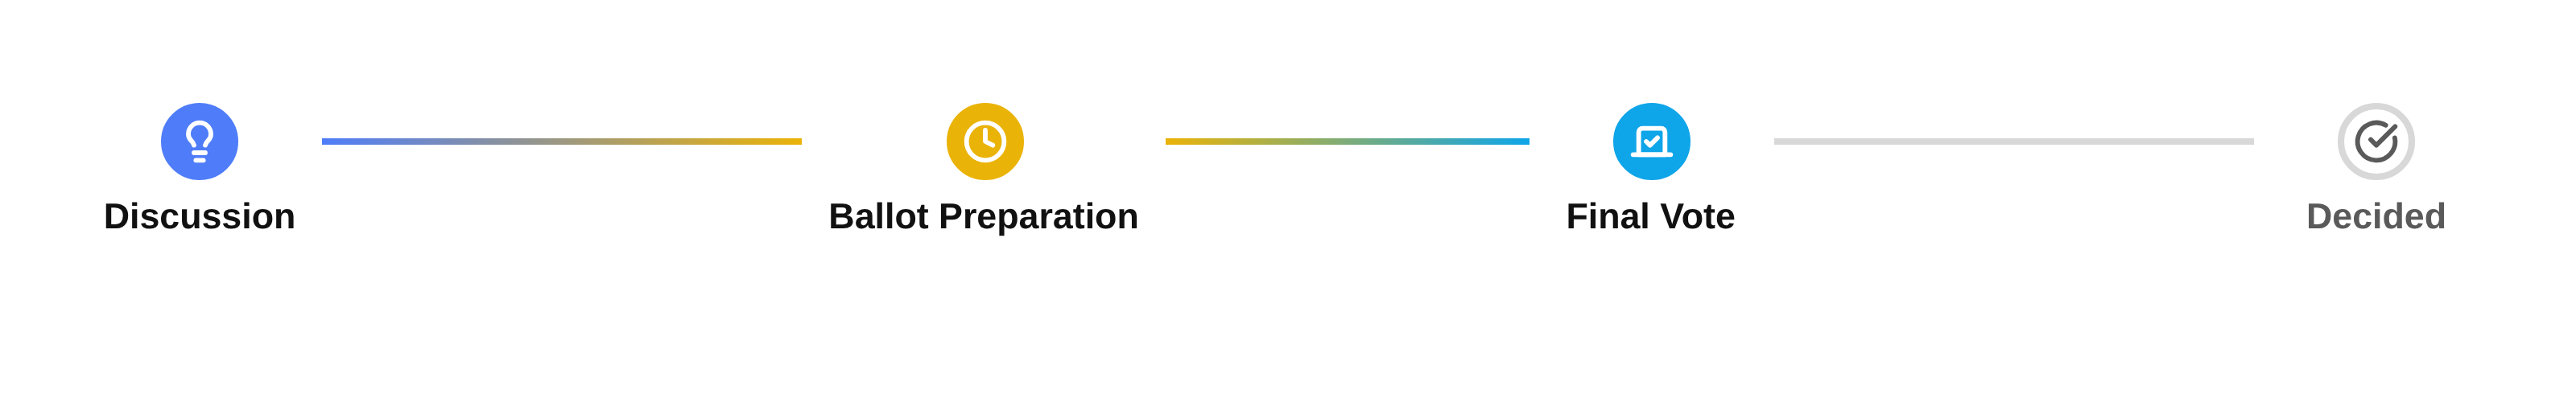
\includegraphics[width=\textwidth]{figures/fig_phase_state_machine.png}
    \caption{The Phases of the Process. The phased progression from problem definition to final collective decision.}
    \label{fig:phase_state_machine}
\end{figure}

The phase structure enables asynchronous work-sharing: participants contribute at their own pace when they have time, and the time-driven transitions ensure the deliberation progresses without requiring synchronous coordination. The detailed phase mechanics (transition logic, duration configuration) are specified in Chapter~\ref{ch:operationalized}.

\section{Design Principles}
\label{sec:design-principles}

Synesis is built upon four design principles, ordered below from the most structurally fundamental to the most interface-specific.

\paragraph{Distributed authority.}
\label{sec:distributed-authority}
Every user has identical capabilities: propose, remix, subscribe, and vote. There are no moderators who curate proposals, no expert judges who select winners, and no institutional gatekeepers who define what counts as a valid contribution. This equal-rights user model distinguishes the platform from nearly all existing participatory tools: Decidim relies on institutional moderators to curate final options; Climate CoLab employed expert judges for winner selection \cite{malone2017contest}; LiquidFeedback's transitive delegation empirically concentrates decision power in a small number of ``super-voters'' \cite{kling2015liquidfeedback}. The platform replaces institutional gatekeeping with transparent, inspectable algorithmic coordination: every system action that affects a proposal's competitive standing is traceable to explicit user actions and documented formulas, never to opaque editorial decisions. The one exception is the administrator role, which configures question parameters (phase durations, ballot size) in the prototype at least. This residual asymmetry is acknowledged in Section~\ref{sec:embedded-politics}. The equal-rights model governs the swappable algorithm architecture and the community-driven thematic management (Chapter~\ref{ch:operationalized}).

\paragraph{Partial contributions as raw material.}
\label{sec:partial-contributions}
The platform expects rough, incomplete fragments, not polished proposals. This is meant to keep the effort of contributing as low as possible. This is the direct operationalization of the ABM's core mechanism: the common knowledge base works \textit{because} partial solutions are stored and re-used across the group \cite{carpentras_empowering_2024}. The entire scaling advantage of remixing over crowdsourcing derives from the fact that each participant's contribution, however incomplete, becomes raw material for others to refine, recombine, and extend. Quality emerges from iterative collective refinement, not individual authoring skill. This principle governs the knowledge base's non-destructive iteration. Both old and new versions coexist, so imperfect contributions carry little risk. This is expected to lower the bar to contribute some raw thought which means potentially greater participation, more creative input and greater work sharing capacity.

\paragraph{Diversity of ideas.}
The platform structurally ensures that distinct perspectives are preserved throughout the deliberation and represented in the final decision. Ideas are grouped thematically via the manual and inheritance based labeling system. The Ballot is computed in a way that no single perspective can dominate it. The exclusiveness rule of the ballot and the cross-perspective routing of the personal window are detailed in Chapter~\ref{ch:operationalized}.

\paragraph{Constrained interaction model.}
\label{sec:positive-only}
The platform provides three user-to-user interaction modes: editing an existing proposal (creating a modified copy), combining two proposals into a synthesis, or creating an entirely new root alternative. Commenting, downvoting, and other reaction mechanisms were removed during iterative development to reduce the complexity of the interface, limit the number of interaction types (which reduced bugs and cognitive load) and produce cleaner telemetry signals for evaluation studies. The consequence of this simplification is that the only way to express disagreement on the platform is to author a constructive alternative. The ABM of Carpentras et al.\ \cite{carpentras_wisdom_2025} also assumes remixing to be the only way for users to interact. The cognitive cost of authoring alternatives compared to simpler reaction mechanisms and how the platform mitigates it are analyzed in Chapter~\ref{ch:operationalized}. The friction that this constraint caused in user studies and its broader implications for the design of the platform interaction are discussed in Chapter~\ref{ch:discussion}.

\section{Shared Knowledge Base}

\subsection{Directed Acyclic Graph as Deliberative Structure}
\label{sec:dag-structure}

At the architectural core of the platform lies a \textbf{Directed Acyclic Graph (DAG)} of proposals. Unlike flat discussion forums, where contributions are organized chronologically or by reply depth, the platform treats every proposal as a \textit{node}, and every evolutionary relationship (edit, combination) as \textit{directed edges}. The resulting structure works like a Git commit history: each proposal records its parentage, and the full graph captures the evolutionary history of the group's deliberation.

This analogy is structurally precise. In Git, developers branch from a shared codebase, iterate independently, and merge their improvements back. The same operations map directly onto the platform's three proposal types: root proposals initialize new branches, edits create single-parent forks that refine an existing idea; and combinations produce multi-parent merges that synthesize elements from competing proposals.

This graph structure provides two critical affordances that flat forums lack. First, \textit{structural lineage}: every proposal's ancestry is explicitly recorded, enabling users to trace how an idea evolved from its original articulation through successive community refinements. Second, \textit{non-destructive iteration}: creating an edit does not modify or suppress the parent; both versions coexist in the graph, and the community's subscription signals determine which variant rises to prominence.

A key limitation distinguishes this from software version control: \textit{semantic merging is unsolved}. In Git, merge conflicts are sometimes detectable because code has formal syntax. In natural-language deliberation, there is no automated way to tell whether two proposals are compatible, contradictory, or orthogonal. The platform therefore relies on human judgment: a Combination's author must manually synthesize the relevant elements of each parent into a coherent new proposal. The system provides the structural scaffold (multi-parent edges) but not the semantic resolution.

The structural logic of the DAG (recombination and incremental improvement in a shared knowledge base) operationalizes the Collective Brain framework introduced in Section~\ref{sec:ci-framework}. It also directly implements the central mechanism of Carpentras et al.'s agent-based model \cite{carpentras_empowering_2024}: a common knowledge base in which partial solutions are stored and re-used across the group, enabling the win-win dynamic between majority and minority proposals that the simulation predicts.
\begin{figure}
    \centering
    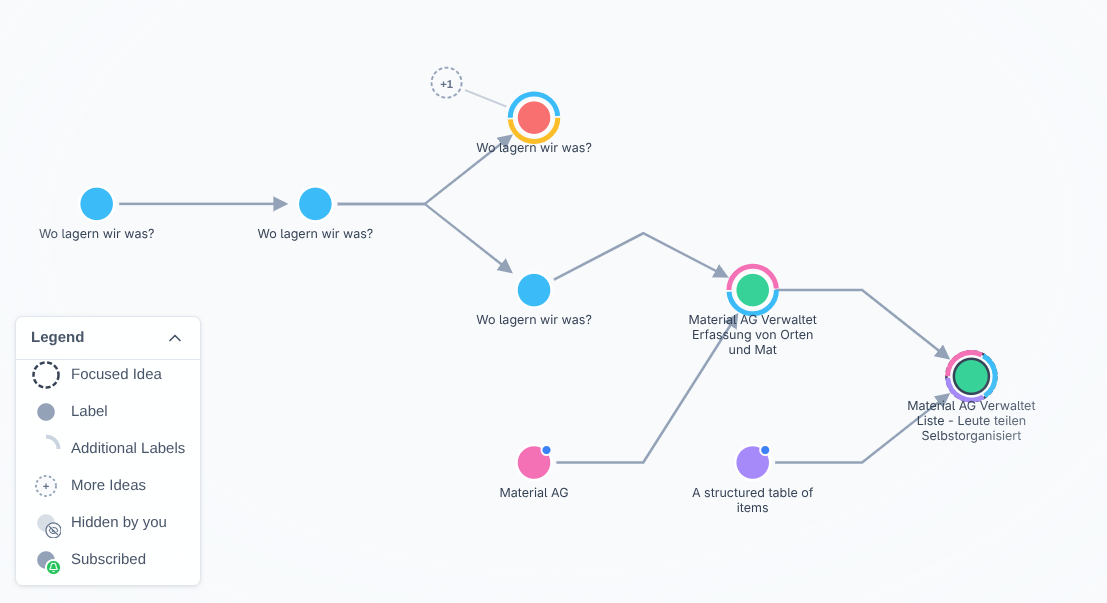
\includegraphics[width=1\linewidth]{figures/User_Study_Generated_DAG_Screenshot.png}
    \caption{The Proposal DAG: structure. This proposal graph was generated by a qualitative user study. The graph shows root nodes (new ideas), edits (single-parent forks), and combinations (multi-parent merges). Proposals are grouped by thematic labels encoded here as colors.}
    \label{fig:proposal_dag}
\end{figure}

\subsection{Asynchronous Work-Sharing - Producing and Sorting the Shared Store}
\label{sec:async-work-sharing}

The proposal DAG constitutes a \textit{shared knowledge base}: a collectively produced, version-controlled repository of ideas, arguments, and syntheses that grows as the community contributes. Each participant's contribution, however partial, becomes available to all others as raw material for further refinement.

The DAG enables \textit{algorithmic attention routing}: the platform's discovery algorithm distributes each user's attention across the shared store, surfacing proposals where their contribution is most needed. Users contribute different kinds of work: posting rough ideas, restructuring unclear proposals, adding missing perspectives, forking ideas to explore alternatives, and synthesizing contributions from multiple authors.

The core scaling challenge this creates is a \textit{distributed evaluation problem}. A deliberation with $N$ participants and $P$ proposals produces an $N \times P$ attention matrix. Full evaluation by every participant (the standard assumption in deliberative assemblies) is infeasible beyond small groups. If we assume users produce a constant amount of proposals on average, this attention matrix scales quadratically with the amount of users in the system. The platform must therefore distribute the evaluation workload so that each proposal receives enough independent assessments to produce a reliable quality signal, while each user evaluates only a tractable subset. This is structurally analogous to the reviewer assignment problem in academic peer review \cite{charlin2013}, where papers must be matched to qualified reviewers under workload constraints, but here in a dynamic, self-organizing context where the ``papers'' (proposals) are created continuously and the ``reviewers'' (users) choose their own engagement.

Surowiecki's four conditions for wise crowds \cite{surowiecki2004} provide the design framework for this distributed evaluation: \textit{diversity of opinion} (users must be routed across multiple perspectives), \textit{independence} (routing must be based on each user's individual state rather than herd signals, to prevent information cascades \cite{lorenz2011social}), \textit{decentralization} (each user draws on their own local knowledge), and \textit{aggregation} (the convergence pipeline transforms individual evaluations into collective signals). The attention-routing algorithm is the mechanism that helps to ensure the diversity and independence conditions are met at the input level, so that the aggregation step produces a reliable output. Carpentras et al.\ \cite{carpentras_wisdom_2025} predict that distributed evaluation with approximately 50 votes per proposal suffices to identify solutions within 90\% of the theoretical optimum under worst-case preference misalignment. Whether this threshold holds with real human evaluators, who vary in engagement, expertise, and attention---is an empirical question that the study's small scale (7--12 participants) can only begin to probe. The platform's two-stage structure (distributed subscription-based evaluation during the Discussion phase, followed by a full ranked ballot during the final Voting phase) structurally mirrors the paper's ``distributed voting followed by full voting'' setup, which improves selection quality beyond distributed voting alone.

This is what makes remixing scalable as a coordination approach: unlike deliberation (which requires everyone in the room) or crowdsourcing (which does not build on prior work), remixing enables structured, asynchronous collaboration on a shared store where each contribution becomes raw material for the next.

\section{The Three-Window Architecture}
\label{sec:three-window}

\subsection{The Tension Between Individual and Collective Perspectives}

The shared knowledge base can be viewed from two perspectives: the \textit{individual perspective}, which asks ``Which ideas are the most relevant to me and where can I contribute the most?'', and the \textit{collective perspective}, which asks ``what are the best ideas of the community?''

These two perspectives are in productive tension. A system optimized purely for personal relevance risks creating filter bubbles that fragment the community into echo chambers. A system optimized purely for collective popularity risks suppressing novel or minority perspectives that have not yet accumulated broad support.

Three distinct mechanisms mediate this tension, each constituting a separate architectural window through which users engage with the shared proposal space. The \textit{Discovery Window} (Section~\ref{sec:personal-window}) routes each user's individual attention across the proposal space. The \textit{Evaluation Window} (Section~\ref{sec:evaluation-window}) aggregates individual endorsements into a community-level signal and drives deliberative dynamics via the Siphon Effect. The \textit{Collective Window} (Section~\ref{sec:collective-window}) crystallizes that signal into a final, diversity-enforced collective aggregated view. Individual actions in the first two windows propagate into the collective output of the third: every subscription updates the Champion rankings, every subscription change updates the Siphon-notification queue, every shift in the Champion set reshapes the ballot. The architecture is designed so that individual agency and collective outcome are tightly coupled, yet structurally separated. Figure~\ref{fig:system-architecture} provides an overview of this architecture and the data flows between its components.

\begin{figure}[htbp]
\centering
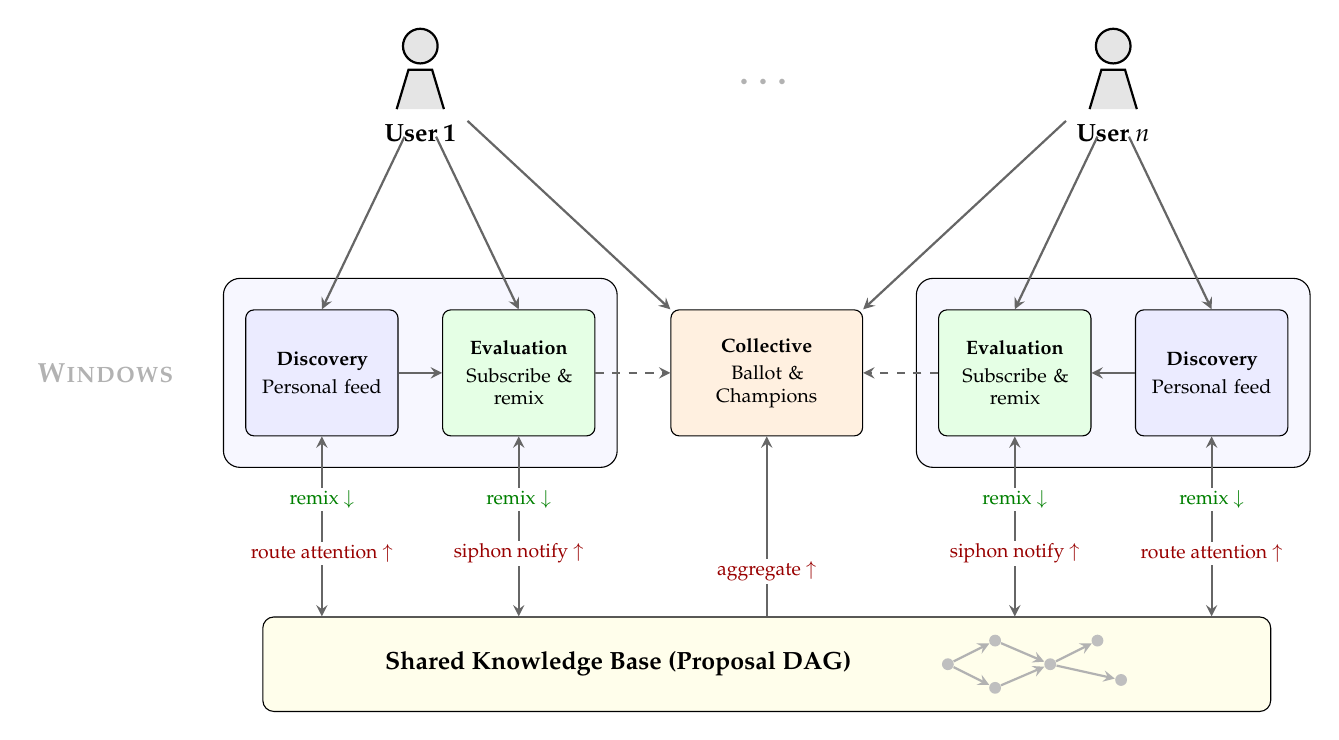
\begin{tikzpicture}[
    >=stealth,
    % Styles
    window/.style={draw, rounded corners=3pt, fill=#1, 
        minimum width=1.8cm, minimum height=1.6cm, font=\scriptsize,
        align=center, text width=1.7cm},
    dagbox/.style={draw, rounded corners=4pt, fill=yellow!8, 
        minimum width=12.8cm, minimum height=1.2cm},
    planelabel/.style={font=\scriptsize\scshape, text=gray!70},
    leveltext/.style={font=\scshape\bfseries, text=gray!60, align=right}
]

% --- Users ---
\node (user1) at (-4.4, 0) {};
\node (userN) at (4.4, 0) {};
\node[font=\LARGE, text=gray!60] at (0, -0.3) {\dots};

% User 1 icon
\draw[thick, fill=gray!20] (-4.4, 0.15) circle (0.22);
\draw[thick, fill=gray!20] (-4.7, -0.65) -- (-4.55, -0.15) -- (-4.25, -0.15) -- (-4.1, -0.65);
\node[font=\small\bfseries, below=0.02cm] at (-4.4, -0.7) {User 1};

% User N icon
\draw[thick, fill=gray!20] (4.4, 0.15) circle (0.22);
\draw[thick, fill=gray!20] (4.1, -0.65) -- (4.25, -0.15) -- (4.55, -0.15) -- (4.7, -0.65);
\node[font=\small\bfseries, below=0.02cm] at (4.4, -0.7) {User $n$};

% --- Level Labels ---
\node[leveltext] at (-8.4, -4.0) {Windows};

% --- Window planes ---
\node[draw, rounded corners=6pt, fill=blue!3, minimum width=5.0cm, minimum height=2.4cm] (box1) at (-4.4, -4.0) {};
\node[draw, rounded corners=6pt, fill=blue!3, minimum width=5.0cm, minimum height=2.4cm] (boxN) at (4.4, -4.0) {};

% --- Windows ---
\node[window=blue!8] (disc1) at (-5.65, -4.0) {\textbf{Discovery}\\[2pt]Personal feed};
\node[window=green!10] (eval1) at (-3.15, -4.0) {\textbf{Evaluation}\\[2pt]Subscribe \&\\remix};

\node[window=green!10] (evalN) at (3.15, -4.0) {\textbf{Evaluation}\\[2pt]Subscribe \&\\remix};
\node[window=blue!8] (discN) at (5.65, -4.0) {\textbf{Discovery}\\[2pt]Personal feed};

\node[window=orange!12, minimum width=2.4cm, text width=2.2cm] (collective) at (0, -4.0) {\textbf{Collective}\\[2pt]Ballot \& Champions};

% --- Arrows from Users to Windows ---
% User 1
\draw[->, thick, gray!80!black] (-4.6, -1.0) -- (disc1.north);
\draw[->, thick, gray!80!black] (-4.2, -1.0) -- (eval1.north);
\draw[->, thick, gray!80!black] (-3.8, -0.8) -- (collective.north west);
% User N
\draw[->, thick, gray!80!black] (4.6, -1.0) -- (discN.north);
\draw[->, thick, gray!80!black] (4.2, -1.0) -- (evalN.north);
\draw[->, thick, gray!80!black] (3.8, -0.8) -- (collective.north east);

% --- Horizontal Influence Arrows ---
\draw[->, thick, gray!80!black] (disc1.east) -- (eval1.west);
\draw[->, thick, gray!80!black, dashed] (eval1.east) -- (collective.west);
\draw[->, thick, gray!80!black] (discN.west) -- (evalN.east);
\draw[->, thick, gray!80!black, dashed] (evalN.west) -- (collective.east);

% --- DAG ---
\node[dagbox] (dag) at (0, -7.7) {};
\node[anchor=east, font=\small\bfseries] at (1.2, -7.7) {Shared Knowledge Base (Proposal DAG)};

% DAG Icon next to text
\begin{scope}[every node/.style={circle, fill=gray!50, minimum size=0.15cm, inner sep=0pt}]
    \node (n1) at (2.3, -7.7) {};
    \node (n2) at (2.9, -7.4) {};
    \node (n3) at (2.9, -8.0) {};
    \node (n4) at (3.6, -7.7) {};
    \node (n5) at (4.2, -7.4) {};
    \node (n6) at (4.5, -7.9) {};
\end{scope}
\begin{scope}[->, thick, gray!60]
    \draw (n1) -- (n2);
    \draw (n1) -- (n3);
    \draw (n2) -- (n4);
    \draw (n3) -- (n4);
    \draw (n4) -- (n5);
    \draw (n4) -- (n6);
\end{scope}

% --- Window <-> DAG connections ---
\draw[<->, thick, gray!80!black] (disc1.south) -- (disc1.south |- dag.north)
    node[pos=0.35, fill=white, inner sep=1pt, font=\scriptsize, text=green!50!black] {remix $\downarrow$}
    node[pos=0.65, fill=white, inner sep=1pt, font=\scriptsize, text=red!60!black] {route attention $\uparrow$};
\draw[<->, thick, gray!80!black] (discN.south) -- (discN.south |- dag.north)
    node[pos=0.35, fill=white, inner sep=1pt, font=\scriptsize, text=green!50!black] {remix $\downarrow$}
    node[pos=0.65, fill=white, inner sep=1pt, font=\scriptsize, text=red!60!black] {route attention $\uparrow$};
\draw[<-, thick, gray!80!black] (collective.south) -- (collective.south |- dag.north)
    node[pos=0.75, fill=white, inner sep=1pt, font=\scriptsize, text=red!60!black] {aggregate $\uparrow$};

% Eval1 <-> DAG (Siphon left)
\draw[<->, thick, gray!80!black] (eval1.south) -- (eval1.south |- dag.north) 
    node[pos=0.35, fill=white, inner sep=1pt, font=\scriptsize, text=green!50!black] {remix $\downarrow$}
    node[pos=0.65, fill=white, inner sep=1pt, font=\scriptsize, text=red!60!black] {siphon notify $\uparrow$ };

% EvalN <-> DAG (Siphon right)
\draw[<->, thick, gray!80!black] (evalN.south) -- (evalN.south |- dag.north) 
    node[pos=0.35, fill=white, inner sep=1pt, font=\scriptsize, text=green!50!black] {remix $\downarrow$}
    node[pos=0.65, fill=white, inner sep=1pt, font=\scriptsize, text=red!60!black] {siphon notify $\uparrow$};

\end{tikzpicture}
\caption{System architecture overview. Multiple users interact with the shared knowledge base through individual \textit{Discovery} and \textit{Evaluation} windows, while observing a shared \textit{Collective Window}. The individual windows feed sequentially into the collective view, driven by user evaluations, which in turn feeds back into the Discovery windows. The Siphon Effect creates a feedback loop: new remixes in the DAG trigger notifications to existing subscribers via their Evaluation window.}
\label{fig:system-architecture}
\end{figure}


\subsection{Window~I: The Discovery Window}
\label{sec:personal-window}

The personal window presents each user with a dynamically ranked perspective on the proposal space, generated by an attention-routing algorithm. The algorithm's purpose is to solve the distributed evaluation problem identified in Section~\ref{sec:async-work-sharing}: it must ensure that every proposal accumulates enough independent assessments while each user evaluates only a tractable subset. We expect the users to handle thematically related proposals better and with more motivation than random proposals that need a lot of effort to grasp each time anew, thus this algorithm should aid users to find their respective niche in the problem solving space.

The algorithm operates on three categories of input: (1)~aggregate proposal statistics available to all users (view counts, subscription counts, thematic groupings), (2)~the individual user's interaction history (which proposals they have viewed, subscribed to, or dismissed), and (3)~the DAG's topological structure (parent--child relationships, label assignments). It is computed entirely on the user's device from server-provided aggregate statistics, a deliberate privacy-by-design choice that ensures no centralised profile of user preferences is ever constructed.

From these inputs, the algorithm produces a personalised ranking that must satisfy the design constraints established in Sections~\ref{sec:async-work-sharing} and~\ref{sec:design-principles}: it must counteract the \textit{first-mover advantage} so that early proposals do not monopolise attention simply by being visible first, it must enforce \textit{cross-label diversity} so that users encounter proposals from multiple thematic groups rather than a single perspective, and it must preserve \textit{independence} by basing routing decisions on each user's individual interaction state rather than on herd signals.

The architecture treats the attention-routing algorithm as a \textit{swappable component} with a well-defined interface: any algorithm satisfying these constraints is a valid candidate for the personal-window role. The specific algorithmic instantiation of this window in our prototype is the PersonalFocus (PF) algorithm, which dynamically surfaces under-explored and structurally diverse proposals. The attention-routing algorithm has no analogue in the ABM of Carpentras et al.\ \cite{carpentras_wisdom_2025}, which assumes that agents access the full proposal space uniformly; it addresses a problem that emerges only at implementation scale, the infeasibility of full or even large amounts of  evaluations and the need to distribute attention without creating first-mover advantage or filter bubbles. The structural requirements and the current heuristic implementation are formalized in Chapter~\ref{ch:operationalized}.

\subsection{Window~II: The Evaluation Window}
\label{sec:evaluation-window}

The Evaluation Window is the platform's primary aggregation mechanism and the structural bridge between individual action and collective outcome. Its surface manifestation is simple: users subscribe to proposals they find valuable, and unsubscribe from proposals they no longer prefer. Beneath this surface, however, each subscription event propagates through the system in two ways.

First, subscription counts constitute the \textit{community signal} from which Champion proposals are elected: the highest-subscribed proposal within each thematic cluster becomes the cluster's representative in the ballot. Second, subscriptions trigger \textit{Siphon notifications}: when a new remix of a proposal arrives, its current subscribers are notified and invited to compare it with the original, optionally migrating their subscription to the refined descendant.

The Evaluation Window is distinct from the Discovery Window in a structurally important sense: the Discovery Window helps users find potentially interesting or important proposals that balance both the user's and the whole community's interests. The Evaluation Window, on the other hand, is a user kept shortlist of proposals to keep tabs on. A user can encounter proposals in various ways, e.g. via the Collective Window and subscribe to it, triggering a full chain of Siphon notifications - entirely independently of the algorithmic Discovery Window. This independence means that the Evaluation Window's dynamics are not contingent on the Discovery Window's algorithm: the convergence mechanism functions even when users browse by recency, by label, or by their own subscription list.

\subsection{Window~III: The Collective Window}
\label{sec:collective-window}

The Collective Window crystallizes the community's aggregated subscription signals into a collectively legitimized running shortlist of best proposals. Its purpose is complementary to the Evaluation Window: where the Evaluation Window accumulates and refines individual endorsements continuously throughout the deliberation, the Collective Window applies a diversity constraint and aggregates these signals.

Two principles govern the design of the Collective Window. First, \textit{competitive selection}: the most subscribed proposals across the community at any given time need to be surfaced. Second, \textit{diversity enforcement}: the collective output must represent distinct perspectives, no single thematic group should dominate. Together, these ensure that the community's strongest \textit{and} most diverse ideas are surfaced, and that the composition of the collective output is governed by the community's own thematic organization rather than by editorial curation.

The specific mechanisms that implement these principles---thematic grouping, leading-idea selection, and the final ballot composition---are detailed in Chapter~\ref{ch:operationalized}.

\subsection{The Siphon Effect: Driving Deliberative Dynamics}
\label{sec:siphon-effect}

The three-window architecture described above provides three complementary perspectives on the same knowledge base at any given moment: novelty discovery, established interest following, and collective  support. 
These windows are constantly moving as the deliberation evolves. The mechanism that drives this is \textbf{active subscription re-evaluation}.

When a new remix is created, the system notifies all current subscribers of the parent proposal, prompting them to compare the original with the improvement and optionally transfer their subscription. Each individual migration updates the user's personal window (they now follow a different proposal's evolution) and because the collective window aggregates subscriptions, shifts the community-level ranking as well. This produces a ``Siphon Effect'': support flows along DAG edges from earlier proposals to their refined derivatives, keeping the deliberation dynamic as the knowledge base grows.

The Siphon Effect as implemented operates independently within each thematic branch. It does not force convergence toward a single idea, but ensures that \textit{within each strand of the deliberation}, support tracks the community's latest and strongest refinements. As a side effect, it also prevents \textit{idea entrenchment}: early proposals cannot indefinitely dominate the collective window simply by having arrived first, because each improvement gives their subscribers an explicit opportunity to move on. The Siphon Effect has no direct analog in Carpentras et al.'s agent-based model \cite{carpentras_wisdom_2025}. The notification mechanics and quantitative dynamics are formalized in Chapter~\ref{ch:operationalized}.

\chapter{System Architecture Operationalized}
\label{ch:operationalized}

The technical implementation of these mechanisms, forming Synesis, is maintained as an open-source project \cite{drp_repo}.

%The central question is: \textit{What is the best structure for iterative ideation from a shared question to a single democratically selected answer?} 

\section{User Interactions and Deliberation Mechanisms}
\label{sec:delib-mechanisms}
The discussion phase, the platform's primary working phase, where all proposal creation, browsing, remixing, combining, and subscription activity occurs, has a very constrained user-to-user interaction mechanism design.

The proposal generation and remixing mechanisms are operationalized via three interaction modes (Section~\ref{sec:positive-only}): (1)~\textbf{Edit}, creating a single-parent fork, (2)~\textbf{Combine}, creating a multi-parent synthesis, or (3)~\textbf{Create Alternative}, authoring a new root proposal with no parents. These are the platform's only user-to-user interaction mechanisms.

Commenting and other contribution mechanisms that do not feed into the proposal graph were removed during development to keep the interaction model minimal and the telemetry interpretable. The only ways for users to interact on the platform are viewing, subscribing, and remixing other users' proposals.

Subscribing to a proposal is a binary toggle between Subscribe ($1$) and Retract ($0$).
In practice, a form of ternary signaling persists through the \textit{subscribe} and \textit{dismiss} (labelled ``Hide'' in the user interface) actions. Subscriptions drive the convergence mechanism (Siphon Effect and Ballot composition), while dismissals serve only as private workspace management. They clean the user's feed without penalizing the proposal in the collective view. 


\section{The Convergence Pipeline}
\label{sec:convergence-pipeline}
This section presents the end-to-end pipeline that transforms individual subscription signals into a collective ranking. The pipeline has four stages: \textit{Subscription as Signal} defines the platform's unit for evaluation, the \textit{PersonalFocus algorithm} routes individual attention to ensure adequate coverage, \textit{Champion Selection} identifies the leading proposal within each thematic group defined by its label, and the \textit{label-exclusive ballot algorithm} assembles a maximally diverse final ballot from the Champions.


\subsection{Subscriptions}
\label{sec:subscription-signal}

The convergence pipeline's input is the \textbf{subscription}: a persistent, binary signal indicating that a user wants to be updated on improvements of a proposal that is treated as an endorsement signal as well. A subscription persists across sessions and can be retracted or migrated to a child proposal at any point during the deliberation. The subscription count is the primary metric driving Champion selection and as a consequence Ballot composition.

A subscription carries dual semantic load: during early development, the platform maintained two separate actions, a lightweight ``like'' (expressing interest without commitment) and a ``subscribe'' (committing to follow a proposal's evolution and receive remix notifications). User testing revealed that non-technical participants found this distinction confusing, and the two actions were merged into a single ``subscribe'' operation. To reduce cognitive load, the platform compresses 'interest' and 'evaluative endorsement' into a single subscription action.
The study's qualitative data (Chapter~\ref{ch:results}) probes whether participants treated subscriptions as evaluative commitments or as lightweight bookmarks.

When a user creates or remixes a proposal, they are automatically subscribed to it, expressing the creator's default endorsement of their own work.
A user who subscribes early and never revisits their decision still counts toward the proposal's standing.
The subscription migration prompting mechanism exists precisely to counteract this stickiness. 

\subsection{Subscription Migration and the Siphon Effect}
\label{sec:siphon-operationalized}
The Siphon Effect (Section~\ref{sec:siphon-effect}) is operationalized through targeted notifications. When a user creates a remix of an existing proposal, all users subscribed to it are notified with a prompt to review the improvement. For users enabling push-notifications for the mobile first progressive web application (PWA) this helps the system to get their attention whenever they have time to evaluate the prompt.

If the user decides the remix is superior, a single action nullifies their original subscription ($0$) and casts a new subscription ($+1$) on the remix. 

\subsection{The Labelling System}
\label{sec:labeling-system}

To organize proposals into ``schools of thought'' without centralized moderation or opaque automated processing, the platform uses a \textbf{deterministic label inheritance system}.
Labels serve two structural functions: they group proposals into thematic categories for browsing, and they partition the proposal space, allowing the label-exclusive ballot algorithm (Section~\ref{sec:ballot-algorithm}) to assemble a final vote from distinct schools of thought. The most subscribed proposal per Label is the Champion and has a possibility to gain a slot on the Ballot. Without labels, the system has no way to ensure that the group's attention is distributed across distinct perspectives.

The labeling rules are purely structural:
\begin{itemize}
    \item When a user creates a \textit{root proposal}, the user has to specify a label to capture its essence. The system \textit{suggests} a label derived from the proposal's title (truncated to 40 characters).
    \item When a user creates an \textit{edit} (single-parent fork), the child proposal inherits all labels from its parent. The primary label defaults to the parent's primary label.
    \item When a user creates a \textit{combination} (multi-parent merge), the child inherits the set union of both parents' labels. The author can add a new label at this point or set the primary label during the combine flow, typically choosing a label that represents the synthesis better.
\end{itemize}

This approach was chosen over automated clustering for three reasons. First, it is \textit{fully transparent}: every label assignment is traceable to an explicit user action (creating a root proposal or defining a custom label). Second, it is \textit{computationally trivial}: no model inference, no training data, no fragile clustering parameters. Third, it \textit{enables deterministic overshadowing}: because children inherit their parents' labels, a child proposal computationally supersedes its parents within the same thematic branch, allowing the ballot algorithm to filter for the most refined version of each idea.

\subsection{Champion Selection}
\label{sec:champion-selection}

Within each semantic label, the pipeline identifies a \textbf{Champion}---the top-ranked proposal per label, displayed as ``Leading Idea'' in the user interface. The engine utilizes a three-tier tie-breaking chain to select the Champion:
\begin{enumerate}
    \item Highest \texttt{subscription\_count}.
    \item Highest \texttt{label\_support\_score}.
    \item Oldest creation timestamp (rewarding the originator if all else is equal).
\end{enumerate}

The \texttt{label\_support\_score} deserves clarification, as it is a non-obvious derived metric. For each label $\ell$, the system first computes $\text{labelAgg}(\ell) = \sum_{p \in P_\ell} \texttt{subscription\_count}(p)$, where $P_\ell$ is the set of all proposals tagged with label $\ell$. Then, for each proposal $p$, the score is defined as:
\begin{equation}
\text{label\_support\_score}(p) = \sum_{\ell \in \text{labels}(p)} \text{labelAgg}(\ell)
\end{equation}
This metric captures the total ecosystem engagement across all topics the proposal addresses. A proposal touching multiple popular labels, typically a Combination that bridges schools of thought, will score higher than a proposal confined to a single niche, rewarding cross-cutting synthesis in the tie-breaking chain. Because combinations inherit the union of their parents' labels (Section~\ref{sec:labeling-system}), multi-parent proposals tend to accumulate many labels as DAGs deepen, giving them higher label support scores. This interaction with the label-exclusive ballot's diversity constraint (Section~\ref{sec:ballot-algorithm}) has scaling implications explored in Section~\ref{sec:sim-three-window}.

\subsection{PersonalFocus Score (For You Feed)}
\label{sec:personalfocus}
The frontend employs a \texttt{PersonalFocus} discovery algorithm to dynamically route attention as an instantiation of the Discovery Window. It is calculated entirely client-side to protect user privacy and reduce server load, the score acts as a localized relevance filter, surfacing under-explored perspectives. Meanwhile, we also allow for the sorting and filtering of the proposals in other ways, like by time or amount of subscriptions.

This section first defines the tracked signals and structural requirements that any attention-routing algorithm must satisfy, then presents the specific heuristic.

\subsubsection{Tracked Signals}
The algorithm operates on five discrete user actions, which are the only behavioral inputs the system records:
\begin{description}
    \item[View:] The user opens a proposal's detail page. Recorded server-side as a \texttt{user\_proposal\_views} entry, increments \texttt{unique\_viewer\_count} on first view per user. Scrolling past a card in the feed does \textit{not} count as a view, it requires deliberate click-level commitment.
    \item[Subscribe:] The user explicitly signals interest and support. Increments \texttt{subscription\_count} on the proposal and updates the user's label affinity profile.
    \item[Retract:] The user withdraws a previous subscription. Decrements \texttt{subscription\_count}.
    \item[Author / Remix:] The user creates a new proposal, optionally with parent references. Creates new DAG nodes and edges.
\end{description}

\subsubsection{Structural Requirements}
\label{sec:structural-requirements}
There are many ways that the discovery window could be implemented. But all algorithms must satisfy the same structural requirements to produce reliable inputs for the convergence pipeline. 
% Not needed in this section :
%Recent CI research underscores why deliberate design of these requirements matters: Centola \cite{centola2022network} demonstrates that network architecture determines whether social influence converges on truth or amplifies errors, and Galesic et al.\ \cite{galesic2023beyond} identify path dependence and premature convergence as recurring failure modes in collective adaptation.
\begin{enumerate}
    \item \textbf{Coverage.} Every proposal must accumulate enough independent evaluations to produce a reliable quality signal. While theorems like Condorcet's \cite{condorcet1785, austensmith1996} assume independent judgments, the platform explicitly routes attention to dynamically manage coverage, intentionally violating strict independence in favor of structural diversity. 
    
    % This probably does not apply to normative questions
    % Crowdsourcing research suggests 3--10 independent evaluations suffice for simple assessment tasks \cite{snow2008cheap}.
    \item \textbf{Distributed specialisation.} Users should have partially overlapping but distinct coverage areas - enough shared evaluations for inter-rater calibration, enough distinct evaluations for breadth.
    \item \textbf{Anti-preferential attachment.} Each evaluation must reduce a proposal's future demand for attention, preventing the first-mover advantage from creating power-law attention distributions \cite{barabasi1999}.
\end{enumerate}


\subsubsection{The Implemented Heuristic}
The specific mathematical weights in this heuristic were derived from the intuition of the designer to balance the structural requirements of the platform prototype. They were then utilized as-is within the bridging simulations, rather than being analytically derived.

The relevance weight combines eight multiplicative parameters:
\begin{align*}
\text{Weight} =\ & (\text{Smoothed Conversion} + \text{Exploration Boost}) \\
&\times \text{Personal Affinity} \times \text{Diversity Boost} \times \text{Bridging Boost} \\
&\times \text{Unseen Multiplier} \times \text{Subscribed Penalty} \times \text{Time Decay}
\end{align*}
Multiplicative composition is chosen deliberately: it allows any single factor to act as a gate that suppresses a proposal's visibility regardless of other factors (e.g., the Subscribed Penalty reduces already-endorsed proposals by 90\%), while logarithmic and square-root dampening on individual terms prevents extreme runaway behavior.
The eight components serve three distinct functional roles:

\textbf{Quality signal.} The \textit{Smoothed Conversion} component $(\text{subs} + 1) / (\text{views} + 5)$ provides a Laplace-smoothed estimate of the fraction of viewers who subscribed. The additive smoothing constants prevent zero-view proposals from producing undefined or extreme scores. Note that the base term uses addition---$(\text{Smoothed Conversion} + \text{Exploration Boost})$---so that even proposals with zero subscriptions receive a non-zero base score from exploration alone. This guarantees that every proposal enters the feed ranking.

\textbf{Exploration mechanisms.} Four components work against idea entrenchment. The \textit{Exploration Boost} $1 / \sqrt{\text{views} + 1}$ creates \textit{anti-preferential attachment} \cite{barabasi1999}: each unique view globally reduces a proposal's future visibility. Unlike standard platforms where popular content attracts more attention (the rich-get-richer dynamic), this inverse square-root decay means that under-viewed proposals are systematically surfaced. The \textit{Unseen Multiplier} ($\times 2.0$ if unseen, $\times 1.0$ if seen) provides a binary novelty premium. The \textit{Subscribed Penalty} ($\times 0.1$ if the user is subscribed, $\times 1.0$ otherwise) suppresses already-endorsed proposals by 90\%, creating a ``consume and move on'' dynamic that frees the user's attention budget for unassessed proposals. The \textit{Time Decay} $1 / \max(1, \log_{10}(\text{hours} + 10))$ applies a slow logarithmic freshness decay.

\textbf{Exploitation--diversity tension.} Three components balance personal relevance against cross-label breadth. The \textit{Personal Affinity} $1 + \ln(\max\text{LabelAffinity} + 1)$ provides exploitation: for each proposal, $\max\text{LabelAffinity}$ is computed as the maximum, across the proposal's labels, of the user's \textit{LabelAffinity} for that label---defined as the number of proposals the user has subscribed to within that label. Logarithmic scaling prevents runaway exploitation. The \textit{Diversity Boost} $1 + 2.0 \times (1/\sqrt{\text{views}+1}) \times (1/\max(1, \text{affinity}))$ provides counter-exploitation: it inversely weights the user's label affinity, so high-affinity labels receive \textit{less} diversity boost while unfamiliar labels receive \textit{more}. This creates a dynamic analogous to patch-leaving in information foraging theory \cite{pirolli1999}: as the user's experience in a thematic ``patch'' increases, the marginal value of further exploration within that patch decreases, and the algorithm redirects attention toward unexplored territory. The \textit{Bridging Boost} $1 + 1.5 \times \text{smoothedConversion} \times \log_{10}(\text{views}+2)$ rewards proposals with high conversion at scale. It is applied to all proposals regardless of parent count, but empirically favors multi-parent merges because merges have a higher probability to inherit subscriptions from multiple lineages and attract views from multiple label communities.


\subsubsection{Heuristic Weight Provenance}
\label{sec:heuristic-provenance}
The specific weights in the current implementation ($2.0$ for the Unseen Multiplier, $1.5$ for the Bridging Boost coefficient, $0.1$ for the Subscribed Penalty, and the additive smoothing constants $+1$ and $+5$ in the Smoothed Conversion) were chosen by \textit{designer intuition} during iterative development and informal testing. They were not calibrated against the agent-based model of Carpentras et al.\ \cite{carpentras_wisdom_2025}, nor were they derived from formal optimization. This is an acknowledged limitation: the heuristic satisfies the structural requirements qualitatively, but the specific parameter values may not be optimal for any given group size or topic complexity. However, the exact instantiation of the PersonalFocus algorithm is consequential, as demonstrated by the quantitative differences in the simulation experiments (Section~\ref{sec:sim-three-window}).

\subsection{The Label-Exclusive Ballot Algorithm}
\label{sec:ballot-algorithm}
The goal of the platform is to lower the bar of participation for influence on the final Ballot's content. This Ballot is a highly curated set of solutions presented to the whole community built from each individuals preferences. The size of the ballot is configurable, the default implementation limits it to seven proposals as a pragmatic design heuristic to mitigate choice overload and ranking fatigue \cite{iyengar2000choice}, loosely informed by the conventional rules of thumb of working-memory \cite{miller1956}.

To prevent a single dominant faction from occupying multiple slots on the ballot with slightly varied versions of the same idea, the system uses a \textbf{label-exclusive} algorithm. 

The algorithm filters all current Champions to those meeting a minimum viability threshold ($\ge 2$ subscribers). It then sorts these candidates descending by the three-tier tie-breaker. Iterating through the sorted list, the algorithm checks if a candidate's inherited labels overlap with \textit{any} label belonging to a proposal already placed on the Ballot. If an overlap is detected, the candidate is discarded. If there is no overlap, it is added to the Ballot, and its labels are marked as ``seen.''

This rigid algorithmic enforcement guarantees maximum label diversity: the community's final attention is distributed evenly across distinct, well-differentiated schools of thought, ensuring that minority perspectives are structurally protected and granted equal visibility in the final deliberative phase. If labels accurately encode semantics this ensures diversity of ideas, but this cannot be guaranteed.

Combining two proposals creates a merged label set which will itself be inherited by any further remix. 
The Ballot's diversity rule enforces label exclusivity. This means if the combination or any of its child proposals gets more subscriptions than a proposal within any of its parent trees, it outcompetes the respective parent tree as well. 
In the limit, if the community's deliberation converges on a genuinely shared understanding and all labels are merged into one, the Ballot would contain a single proposal---consensus would emerge organically from the labeling system's structural logic without ever imposing a limitation on contradicting proposals. Figure~\ref{fig:label-domination} illustrates how label inheritance through multi-parent combinations can lead to ballot domination.

\begin{figure}[htbp]
\centering
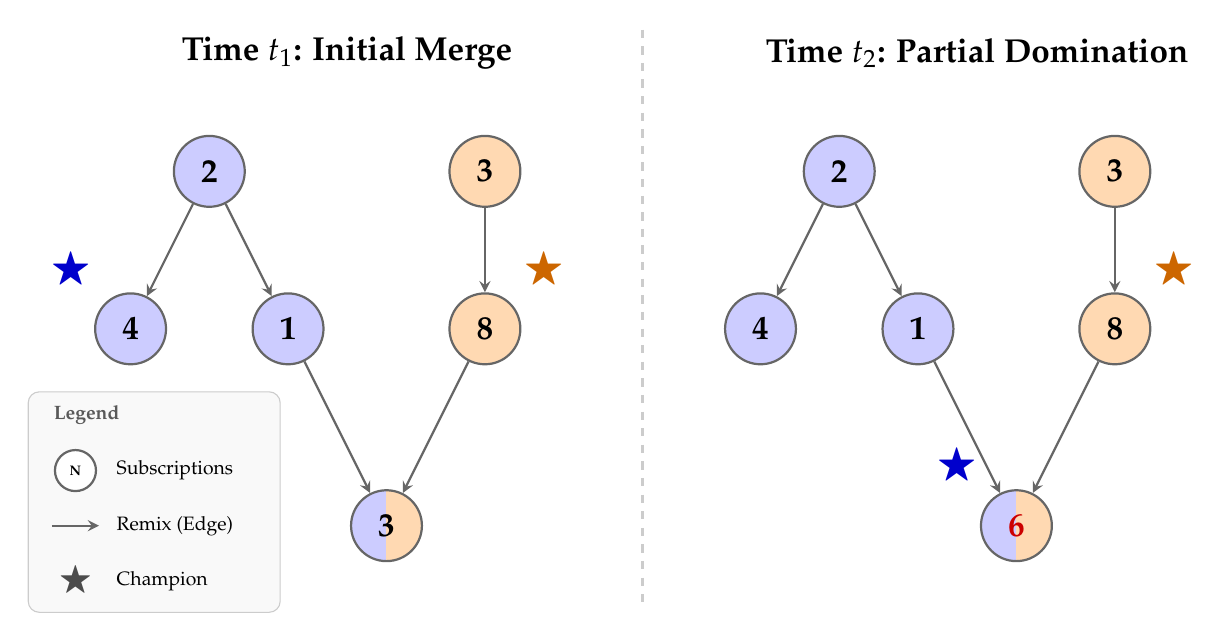
\begin{tikzpicture}[
    >=stealth,
    bluenode/.style={circle, draw=black!60, thick, fill=blue!20, minimum size=0.9cm, font=\large\bfseries},
    orangenode/.style={circle, draw=black!60, thick, fill=orange!30, minimum size=0.9cm, font=\large\bfseries},
    combonode/.style={circle, draw=black!60, thick, minimum size=0.9cm, font=\large\bfseries,
        path picture={
            \fill[blue!20] (path picture bounding box.south west) rectangle (path picture bounding box.north);
            \fill[orange!30] (path picture bounding box.south) rectangle (path picture bounding box.north east);
        }
    },
    edge/.style={->, thick, gray!80!black},
    champlabel/.style={font=\small\bfseries}
]

% ===== Left Side: Initial Merge =====
\node[font=\large\bfseries] at (-3.75, 3.5) {Time $t_1$: Initial Merge};

% Blue graph (forked)
\node[bluenode] (bl_root) at (-5.5, 2) {2};
\node[bluenode] (bl_c1) at (-6.5, 0) {4};
\node[bluenode] (bl_c2) at (-4.5, 0) {1};
\draw[edge] (bl_root) -- (bl_c1);
\draw[edge] (bl_root) -- (bl_c2);

% Orange graph
\node[orangenode] (or_root) at (-2.0, 2) {3};
\node[orangenode] (or_c1) at (-2.0, 0) {8};
\draw[edge] (or_root) -- (or_c1);

% Combination node
\node[combonode] (combo_L) at (-3.25, -2.5) {3};
\draw[edge] (bl_c2) -- (combo_L);
\draw[edge] (or_c1) -- (combo_L);

% Champions Left
\node[text=blue!80!black, font=\Large] at ([xshift=-12pt, yshift=12pt]bl_c1.north west) {$\bigstar$};
\node[text=orange!80!black, font=\Large] at ([xshift=12pt, yshift=12pt]or_c1.north east) {$\bigstar$};


% ===== Right Side: Partial Domination =====
\node[font=\large\bfseries] at (4.25, 3.5) {Time $t_2$: Partial Domination};

% Blue graph (forked)
\node[bluenode] (br_root) at (2.5, 2) {2};
\node[bluenode] (br_c1) at (1.5, 0) {4};
\node[bluenode] (br_c2) at (3.5, 0) {1};
\draw[edge] (br_root) -- (br_c1);
\draw[edge] (br_root) -- (br_c2);

% Orange graph
\node[orangenode] (or_root_R) at (6.0, 2) {3};
\node[orangenode] (or_c1_R) at (6.0, 0) {8};
\draw[edge] (or_root_R) -- (or_c1_R);

% Combination node
\node[combonode] (combo_R) at (4.75, -2.5) {\textcolor{red!80!black}{6}};
\draw[edge] (br_c2) -- (combo_R);
\draw[edge] (or_c1_R) -- (combo_R);

% Champions Right
\node[text=blue!80!black, font=\Large] at ([xshift=-12pt, yshift=12pt]combo_R.north west) {$\bigstar$};
\node[text=orange!80!black, font=\Large] at ([xshift=12pt, yshift=12pt]or_c1_R.north east) {$\bigstar$};

% Separation line
\draw[dashed, thick, gray!40] (0, 3.8) -- (0, -3.5);

% ===== Legend =====
\begin{scope}[shift={(-7.8, -0.8)}]
    \draw[rounded corners=4pt, fill=gray!5, draw=gray!40] (0, 0) rectangle (3.2, -2.8);
    \node[anchor=west, font=\scriptsize\bfseries, text=gray!70!black] at (0.2, -0.3) {Legend};
    
    \node[circle, draw=black!60, thick, fill=white, minimum size=0.4cm, font=\tiny\bfseries] at (0.6, -1.0) {N};
    \node[anchor=west, font=\scriptsize] at (1.0, -1.0) {Subscriptions};
    
    \draw[->, thick, gray!80!black] (0.3, -1.7) -- (0.9, -1.7);
    \node[anchor=west, font=\scriptsize] at (1.0, -1.7) {Remix (Edge)};
    
    \node[text=gray!60!black, font=\large] at (0.6, -2.4) {$\bigstar$};
    \node[anchor=west, font=\scriptsize] at (1.0, -2.4) {Champion};
\end{scope}

\end{tikzpicture}
\caption{Label inheritance and partial domination. Labels are represented by colors (e.g., blue and orange). Subscription counts are shown inside the nodes. \textbf{Left ($t_1$):} A combination node merges a proposal from the blue label (1~sub) and the orange label (8~subs), inheriting both labels. With 3~subscriptions, it is not the champion of either label. \textbf{Right ($t_2$):} The combination node gains subscriptions, reaching 6. This exceeds the highest-ranked pure blue proposal (4~subs), making the combination the new champion of the blue label. However, it still trails the highest-ranked pure orange proposal (8~subs), which remains the orange champion. The combination thus dominates the ballot slot for one of its labels but not the other.}
\label{fig:label-domination}
\end{figure}


\paragraph{Boundary conditions.}
The label-exclusive rule creates edge cases that must be acknowledged. First, if fewer Champions meet the viability threshold ($\geq 2$ subscribers) than the Ballot size allows, the Ballot will contain fewer than seven entries. Second, if aggressive label merging reduces the label space to a single dominating label, the Ballot will by design contain just a single proposal. This means the Ballot algorithm's diversity guarantee depends on the community maintaining meaningful thematic distinctions. Third, Combinations that inherit labels from multiple parents may block large portions of the label space: a proposal tagged with three labels prevents up to three other Champions from entering the Ballot, potentially over-representing the cross-cutting synthesis at the expense of narrower perspectives. Whether this trade-off is acceptable (rewarding synthesis at the cost of specialist representation) is a design judgment rather than an algorithmic inevitability.

\section{The Decision Mechanism: Forming the Ballot and Voting}
\label{sec:decision-mechanism}

\subsection{Ballot Preparation Phase}
When the Discussion deadline elapses, the system enters the Ballot Preparation phase. All proposal creation is disabled only subscriptions can be changed to influence the Ballot's composition. So this phase serves as a final review and collective formation of the Ballot before all users are prompted to vote on the final selection.

\subsection{Borda Count Scoring}
\label{sec:voting-phase}
Once the Ballot Preparation phase expires, all proposals are frozen and the platform transitions to the Final Vote phase. The system employs a \textbf{strict Borda count} \cite{borda1781} for the final preference aggregation. Given $n$ proposals on the ballot, a voter's rank $r$ for a proposal awards $n - r + 1$ points: first place receives $n$ points, second place receives $n - 1$, and so on down to $n$th place receiving $1$ point. The tie-breaking hierarchy for the final ranking is:
\begin{enumerate}
    \item Highest \texttt{bordaScore} (descending).
    \item Highest \texttt{firstPlaceVotes} (descending).
    \item Highest \texttt{totalVotes} (descending).
\end{enumerate}

The engine also computes the maximum possible score (= $n \times \text{activeVotes}$) for normalization and a \texttt{rankDistribution} array tracking how many ballots placed each proposal at each rank position, enabling stacked bar chart visualizations of preference composition.

The choice of Borda count is deliberate. As a consensus-seeking method, Borda favors broadly acceptable solutions over polarizing ones: a proposal benefits from being ranked highly across many ballots rather than being one faction's top pick, aligning with the platform's constructive ethos. With at most seven candidates, the ballot set is small enough that strategic manipulation (``burying'' a competitor by ranking them last) is both less impactful and more easily detectable than in large-field elections. The Borda count also produces a complete ordering of all options, enabling the community to see not only the winner but the full preference landscape.

\subsection{Results and Archive}
When the Voting deadline is reached, the system tallies all Borda ballots and transitions the question to its terminal Decided state. The winning proposal is declared and highlighted in the results view. All proposals, their DAG lineage, subscription histories, and voting data are preserved as a permanent, read-only archive of the community's deliberative process. Detailed ballot interaction design (randomized presentation order, drag-and-drop ranking, abstention handling, re-voting) and results presentation are documented in the open-source repository.

\section{User Interface Implementation}
\label{sec:interaction-model}
In the main workspace view of a question, several tabs are visible at the bottom of the screen (Figure~\ref{fig:window-view-implementation}) corresponding to the three windows mentioned earlier, as well as a general question overview page that explains the system and provides some aggregate metrics about the process of finding an answer.

\begin{figure}
    \centering
    
\includegraphics[width=0.5\linewidth]{figures/Bottom_Nav_Bar.png}
    \caption{The Tab-View when entering a question workspace. "Discover" is the instantiation of the Discovery Window, "Subscriptions" is the Evaluation Window, and "Ballot" is the Collective Window, doubling as the final ballot view.}
    \label{fig:window-view-implementation}
\end{figure}

\subsection{Discovery Window UI}

The Discovery Page provides several scrollable list views as filterable feeds of proposal cards for browsing and rapid assessment. Users can switch between sub-tabs (All, For You, Hidden), apply filters (Supported, Leading Ideas, On Ballot, Unseen, Combinations, Improvements, Label-specific), and sort by popularity, recency, or personal relevance (Figure~\ref{fig:discovery-window-screenshot}).

\subsection{Detail View}
The \textbf{Detail View} presents a single proposal's complete content, its related ideas (lineage), the author's rationale for the last change, the further edits of the selected proposal, and how it ranks within its label. It also allows users to edit the proposal (creating a remix of it) via the push of a button, opening an inline editing interface. This should make it as easy as possible to submit one's own small edits.

\paragraph{The DAG View: Local-Neighbourhood Navigation}
\label{sec:graph-view}
Rather than presenting a full overview of the proposal DAG, the platform embeds a \textbf{local-neighborhood graph} within the Detail View (see Figure~\ref{fig:mobile-detail-dag-view}), showing the selected proposal's immediate structural context: ancestor chains, child iterations, and topical peers. No full-graph overview is exposed to users. 

This design choice is grounded in HCI research on graph visualization complexity. Ghoniem et al.\ \cite{ghoniem2005readability} demonstrated in a controlled experiment that node-link diagram readability degrades significantly beyond approximately 20 vertices for most analytical tasks. Van Ham and Perer \cite{vanham2009search} proposed ``search, show context, expand on demand'' as an alternative to Shneiderman's \cite{shneiderman1996eyes} ``overview first'' mantra, arguing that a local-neighborhood view anchored to a node of interest is more effective for users with a specific target. The platform implements this paradigm: the graph appears on the detail page, anchored to the selected proposal, showing where the idea comes from and what has evolved from it, without requiring the user to parse the full deliberation topology.

\begin{figure}[htbp]
  \centering
  \begin{subfigure}[t]{0.45\linewidth}
    \centering
    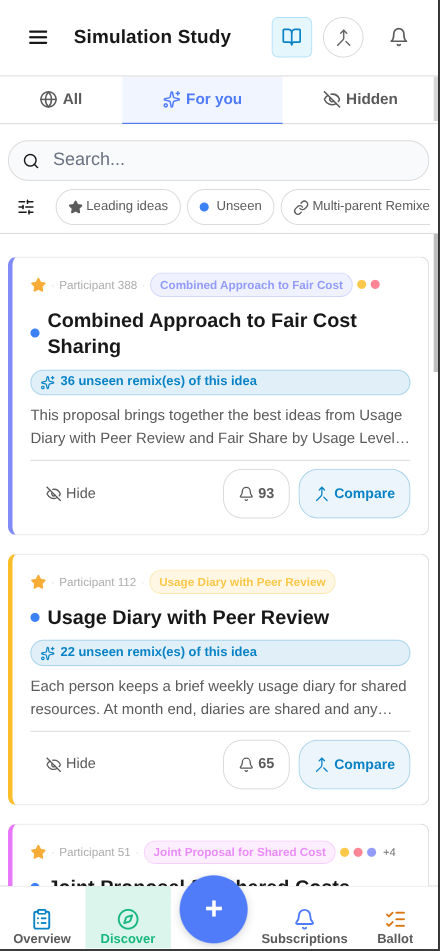
\includegraphics[width=\linewidth]{figures/discovery_feed.png}
    \caption{Discovery Window with filterable feeds, including the PersonalFocus-ranked ``For You'' feed}
    \label{fig:discovery-window-screenshot}
  \end{subfigure}
  \hfill
  \begin{subfigure}[t]{0.45\linewidth}
    \centering
    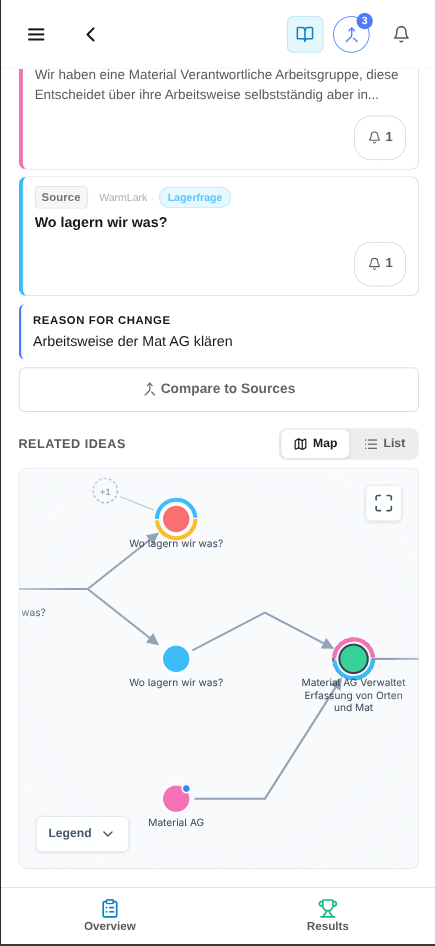
\includegraphics[width=\linewidth]{figures/DAG_view.png}
    \caption{Local-neighborhood graph view on the Detail View}
    \label{fig:mobile-detail-dag-view}
  \end{subfigure}
  \caption{Mobile interface views: (a)~the Discovery feed and PersonalFocus ranking (For you tab), and (b)~the local DAG neighbourhood graph embedded within the Detail View.}
  \label{fig:mobile-views}
\end{figure}

\subsection{Notification-Driven Engagement}
The platform is designed as a mobile-first, notification-driven application. Users receive targeted notifications when proposals they subscribe to are remixed (the Siphon Effect), when phase deadlines approach, and when their supported proposals enter the final ballot. These notifications distribute cognitive contribution across multiple short sessions rather than requiring a single sustained effort.

% --- CHAPTER 4 --- 
\chapter{Evaluation Methodology}
\label{ch:methodology} 

\section{Research Design Overview}
The evaluation follows a design-science research strategy \cite{hevner2004design}, the primary contribution is the design artifact (Synesis), and the evaluation generates design knowledge through iterative deployment with real community groups. The empirical work comprises a formative usability evaluation, a pilot deployment with the research group's own colleagues, and two community deployments with pre-existing groups, each cycle informing design changes for the next. Each deployment constitutes a single case study of a distinct platform version in a distinct community context, the three cases are analyzed individually rather than as an aggregated sample. To bridge the gap between small-scale human deployments and the platform's expected behavior at scale, the empirical work is complemented by multi-agent simulations acting as a comparative baseline.

This evaluation does not use a controlled experiment with treatment and control conditions. Under the design-science frame, the absence of a control group is expected: the evaluation's purpose is to identify whether the artifact achieves its design objectives and what design problems emerge, not to demonstrate superiority over alternatives. The agent-based simulation predictions of Carpentras et al.\ \cite{carpentras_empowering_2024, carpentras_wisdom_2025} provide the theoretical motivation for the design. The evaluation characterizes how human behavior departs from the simulation's assumptions, generating design knowledge for future iterations (Section~\ref{sec:baseline-comparison}).

The research questions (Section~\ref{sec:research-questions}) are primarily concerned with \textit{how} the platform shapes deliberation and \textit{what design friction emerges}, questions best answered through rich qualitative data triangulated with behavioral telemetry, not through statistical hypothesis testing on small samples.

This evaluation takes place within what Cornwall \cite{cornwall2004} would classify as an \textit{invited space}: the researcher defines the question, recruits participants, and sets the timeline. The platform is designed as infrastructure for \textit{popular spaces}, genuinely bottom-up, community-initiated collective decision-making. This limitation is treated as a design finding for RQ1: the platform's question candidate phase, in which the group votes on which questions to pursue, was not implemented in the prototype, and questions were instead pre-selected through facilitated group discussion. The empirical evaluation therefore covers the Discussion, Ballot Preparation, and Final Vote phases of the platform lifecycle, but not the question-selection phase. These limitations are revisited in Chapter~\ref{ch:discussion}.

Finally, the researcher's dual role as platform developer and study facilitator must be acknowledged. This is standard in design-science Master's theses but creates a risk of confirmation bias in qualitative coding. To mitigate this risk, the qualitative coding framework explicitly includes dedicated negative-case codes (e.g., ``didn't know where to start,'' ``notification not working,'' ``missing the ability to say no'').

\section{Study Context and Participants}
The platform is evaluated through an iterative design cycle: a formative usability evaluation on an early prototype, a pilot deployment with the research group's colleagues, and two community deployments with pre-existing groups addressing real organizational problems.

\subsection{Formative Evaluation}
\label{sec:formative-eval}
A single shoulder-looking session was conducted in May~2025 with one participant on an early desktop prototype populated with 51~LLM-generated proposals. The participant was asked to orient themselves on an existing problem, distributing costs for shared items in a flat, and to contribute to it while thinking aloud. The interaction barriers identified during this session informed several interaction design changes deployed prior to the main community studies, detailed in Section~\ref{sec:usability-friction}.

\subsection{Pilot Study: Office Study Group}
\label{sec:pilot-study}
The pilot deployment involved the research group's own office colleagues over 12~days in July~2026. Three questions of deliberately different types were posed: a logistical planning task (retreat activities), a social coordination task (Christmas dinner), and an adversarial stress-test task where participants were prompted to try and break the system (reducing car use in Z\"urich). The English-language deployment validated the full platform lifecycle: all three questions progressed through Discussion, Ballot Preparation, Final Vote, and Decided phases. The pilot served a dual purpose: validating the end-to-end pipeline under controlled conditions and gathering structured feedback that informed the interface changes deployed in the subsequent community studies, documented in Section~\ref{sec:usability-friction}. Data from the Pilot Study was used solely to inform design iterations and is excluded from the main quantitative analysis in Chapter~\ref{ch:results}.

\subsection{Study 1: WG Studiengruppe}
\label{sec:study-wg-studi}
The first community deployment involved a flat-sharing group of 11~consenting participants over 12~days in July--August~2026. The group used the platform to collaboratively address one normative question, how to fairly distribute costs for shared household purchases, defined through group discussions beforehand. This mixed-language deployment served as the first test with a community group outside the research team, providing initial data on the topology of the shared knowledge base (DAG), subscription dynamics, and the Siphon Effect, under conditions where the question carried genuine stakes for participants.

\subsection{Study 2: WG-Netz Winterthur}
\label{sec:study-wg-netz}
The second community deployment involved a pre-existing local community network of 12~consenting participants over 19~days in August~2026. The group addressed two real community coordination problems: defining the network's identity and role in the city, and designing a system for sharing material resources across member households. Both questions were normative, involving competing values and interests with no objectively correct answer. This addresses the concern raised in the collective intelligence literature (Section~\ref{sec:ci-framework}) that epistemic puzzle tasks do not adequately test democratic deliberation. The deployment represents the most realistic evaluation context: the questions were genuine, the participants had a real stake in the outcomes, and the group was large enough to observe the platform's convergence mechanisms.

\subsection{Participants}
\label{sec:participants}
Across all deployments, 30~participants consented to data collection (7~pilot, 11~Study~1, 12~Study~2). Inclusion criteria: fluent in English or German, aged 18 or older. No vulnerable populations were included. Participants were recruited via direct outreach to organizational groups.

Participation was entirely voluntary and uncompensated. This design choice is deliberate: participants engaged because they are genuinely interested in using the platform to solve a real problem, not because of financial incentives. This improves ecological validity but introduces a self-selection bias toward motivated, literate participants, a limitation that must be considered when interpreting results related to usability and accessibility (RQ3). 


\section{Data Collection Methods}

\subsection{Asynchronous Group Deployments}
\label{sec:method-a}
Organizational groups were given access to the platform to collaboratively address a prompt over a set period (12--19 days in the reported studies). During this period, participants interacted with the platform at their own pace, reading proposals, subscribing, dismissing, editing and combining, and eventually casting ranked ballots. Following the deployment, participants completed a digital survey containing the System Usability Scale (SUS) \cite{brooke1996sus} and open-ended qualitative questions covering five dimensions:
\begin{enumerate}
    \item \textbf{Building on Ideas:} Did the platform make it easy to build upon (``remix'') other people's proposals?
    \item \textbf{Convergence Process:} How did the group move from many proposals to one final idea? Which platform features helped or hindered convergence?
    \item \textbf{Finding Quality:} How did participants decide their ranking, selection, or point distribution when choosing ``high-quality'' ideas? Did the system make this easy?
    \item \textbf{Fairness and Legitimacy:} Do participants feel the final solutions fairly represent the group's input? Why or why not?
    \item \textbf{Improvements:} What features do participants wish the platform had?
\end{enumerate}

\subsection{Synchronous Observation Sessions}
\label{sec:method-b}
To complement the asynchronous deployment data, individual ``shoulder viewing'' sessions were conducted in person. Participants were asked to share their screen and ``think aloud'' \cite{ericsson1993protocol} while navigating the platform: verbalising what they were looking at, what they were trying to do, and what confused them.

One such session was conducted (Section~\ref{sec:formative-eval}), using the early desktop prototype with LLM-simulated content. Because this session predated all three deployments and used synthetic rather than community-generated content, it functiond as a \textit{formative} usability evaluation (identifying interaction barriers that informed subsequent design iterations, detailed in Section~\ref{sec:usability-friction})---rather than as a concurrent summative data source. The post-session interview was documented in a structured observation report; no screen recording was retained per the ethics protocol. In addition, several informal think-aloud observation sessions were conducted during the development phase to iteratively refine the interface, though these were not subjected to formal qualitative coding.

\subsection{Platform Telemetry}
\label{sec:telemetry}
Throughout all deployments, the platform automatically logged interaction data with timestamps. This included submitted text (proposals, remixes, combinations), pseudonymised user identifiers, page navigation and routing behavior, subscription and dismissal events, notification delivery and action status, ballot submissions and updates, and session timing. This telemetry provides the behavioral data, which may be used to calibrate simulation studies as well as ground the qualitative survey data.

\section{Multi-Agent Simulation Testbed}
\label{sec:method-c}
A multi-agent computational testbed was developed to generate dummy data as well as to exercise the platform's convergence mechanics under controlled conditions before, during, and after human deployments. The simulation system populated a live instance of the platform with synthetic but behaviorally calibrated deliberation activity, serving three methodological functions.

\paragraph{Integration testing of the convergence pipeline.}
Before exposing the platform to human participants, the simulation engine exercised every state-transition pathway (proposal creation, remixing, merging, subscribing, subscription retraction), and the server-side convergence pipeline (score recalculation, Champion election, Ballot composition, phase transitions) under load conditions exceeding those achievable in small-group studies (up to 100~concurrent agents over 30~simulated days). Critically, agents submitted all mutations \textit{through the same API surface as real users}. All business logic (score recalculation, label assignment, phase transition evaluation, notification generation) was executed server-side by the same code that processes human actions. The simulation did not make direct database writes for core domain actions. Feed ranking was the sole exception: the PersonalFocus algorithm is replicated as a local Python port to avoid HTTP overhead during high-throughput runs (detailed in the Agent decision model paragraph below). This ensured that all state-changing behavior observed in simulation was representative of production behavior.

\paragraph{Generating realistic initial conditions.}
Simulated runs pre-populated the platform with a topically coherent proposal graph, complete with remixed variants, merged syntheses, and vote distributions, such that participants in the formative evaluation encountered a non-empty, contextually plausible workspace. This eliminated the cold-start problem and allowed the researcher to observe how users interacted with an already-active deliberation. Content is generated either via an LLM (GPT-4.1-mini) conditioned on a generic participant role description, or via deterministic fallback templates in German and English.

\paragraph{Behavioral calibration from empirical data.}
After the user studies had been conducted, the simulation's agent model was calibrated from the WG~Studiengruppe deployment (Study~1). The power-user ratio, proposals per user, subscription retraction rate, and the root proposal ceiling were derived directly from this human telemetry. This empirical calibration established a \textit{synthetic behavioral baseline}: deviations between simulated and observed action distributions, convergence trajectories, or engagement curves provided quantitative evidence of how human deliberation differed from the calibrated agent model.

\paragraph{Agent decision model.}
Each simulated agent executed a four-phase decision pipeline per session (full parametric specification in Table~\ref{tab:sim-calibration}; pipeline detail in Appendix~\ref{sec:appendix-agent-pipeline}), structurally mirroring the human interaction flow:
\begin{enumerate}
    \item \textbf{Root Creation Check:} The agent independently evaluates whether to contribute a new root proposal, damped by the global population of roots and its own authorship history to prevent runaway creation.
    \item \textbf{Bounded-Attention Pool Compilation:} To mirror human cognitive constraints, the agent is presented with a bounded pool of at most 11~candidates drawn from the three interface channels: Siphon notifications, Ballot members, and PersonalFocus-ranked feed items. 
    \item \textbf{Target Selection:} The agent samples $k$ proposals from this pool to evaluate. It greedily selects the proposals with the highest perceived utility. following the Carpentras comparison model \cite{carpentras_wisdom_2025}. In quality-blind ablation runs, it selects targets using HCI and information-retrieval-grounded attention weights \cite{pirolli1999, joachims2005accurately}.
     \item \textbf{Action Selection:} For each selected target, the agent independently rolls to remix, combine, or subscribe. Retractions are not rolled independently; they occur exclusively via the Siphon subscription-migration pathway when a child proposal exhibits higher perceived utility than its parent. Invalid actions (e.g., subscribing to an already-supported proposal) are silently discarded rather than falling back to alternative choices.
\end{enumerate}

The PersonalFocus feed ranking was computed by a local Python port of the production algorithm, ensuring consistent ranking logic while avoiding HTTP overhead during high-throughput runs. All mutations (proposal creation, voting, subscription changes) were submitted through the platform's standard API endpoints.

\paragraph{Reproducibility and parametric experimentation.}
All agent-side stochastic processes (engagement rolls, action selection, target selection, session budget assignment, quality draws) used a single seeded random instance (seeds: 42, 99, 137), ensuring that the decision sequence was deterministic for a given seed and configuration. Two residual sources of non-determinism existed: dummy proposal text varied across runs (synthetic text is used in lieu of LLM generation to isolate structural behavior and avoid unnecessary API overhead without impacting the decision model), and the simulation start timestamp defaulted to wall-clock time when not explicitly specified. The simulation supported batch experiments via JSON configuration files, enabling systematic variation of agent counts, PF parameters, and mechanism ablations. Table~\ref{tab:sim-suite} summarizes the experiment suite.


\paragraph{Quality model.}
All three simulation study suites (\texttt{scaling\_frontier}, \texttt{three\_window}, \texttt{siphon\_ablation}) used a quality-aware agent utility model following Carpentras et al.\ \cite{carpentras_wisdom_2025}: each agent evaluated proposals via $u_i(s) = q(s) + \varepsilon_i(s)$, where $u_i(s)$ represents the agent's \textit{perceived} quality of the proposal, derived from the latent true quality $q(s)$ plus individual noise $\varepsilon_i(s) \sim N(0, 0.5)$, drawn once per agent--proposal pair and cached for the duration of the run. This produced stable per-agent preferences, modeling taste heterogeneity rather than evaluation noise. Latent quality $q$ was deterministically assigned from DAG topology: root proposals drew $q \sim |N(0,1)|$; single-parent remixes drew $q = \max(0, q_{\text{parent}} + N(0, 0.5))$; multi-parent combinations drew $q = \max(q_{\text{parents}}) + |N(0, 0.3)|$.


\begin{table}[ht]
\centering
\caption{Simulation experiment suite (90~runs total). All runs simulate 30~days of agent activity and are calibrated on the human user studies. PF = PersonalFocus.}
\label{tab:sim-suite}
\small
\begin{tabular}{l r l l l}
\toprule
\textbf{Study} & \textbf{Runs} & \textbf{Focus} & \textbf{PF} & \textbf{Quality} \\
\midrule
\texttt{scaling\_frontier}    & 54 & 3 regimes $\times$ 6 $N$ $\times$ 3 seeds  & PF / Random / Newest & Yes \\
\texttt{three\_window}         & 24 & 4 configs $\times$ 2 $N$ $\times$ 3 seeds  & On/Off $\times$ Ballot On/Off & Yes \\
\texttt{siphon\_ablation}     & 12 & ON/OFF $\times$ 2 $N$ $\times$ 3 seeds     & Default & Yes \\
\bottomrule
\end{tabular}
\end{table}


\noindent Three \textit{selection efficiency} metrics were used throughout the simulation results (Section~\ref{sec:sim-design-contract}):
\begin{itemize}
    \item \textbf{Ballot Selection Efficiency} ($\eta_{\text{ballot}}$): mean quality of ballot proposals divided by maximum available quality.
    \item \textbf{Top-K Selection Efficiency} ($\eta_{\text{topK}}$): mean quality of the $K$ most-subscribed proposals divided by maximum available quality.
    \item \textbf{Top-1 Selection Efficiency} ($\eta_{\text{top1}}$): quality of the single most-subscribed proposal divided by maximum available quality.
\end{itemize}

\noindent Full parametric specification and the complete decision pipeline are provided in Appendix~\ref{sec:appendix-calibration}--\ref{sec:appendix-agent-pipeline}.

\section{Analytical Framework}
The analysis combined telemetry-derived metrics with qualitative coding to address each research question from multiple angles. Given the small sample sizes (7--12 participants per group), the telemetry metrics were used \textit{descriptively}, to characterize the structural properties of deliberation, rather than for statistical hypothesis testing.

\subsection{Telemetry-Derived Metrics}
\label{sec:telemetry-metrics}
The following objective metrics were computed from platform logs, grouped by the design objective they evaluated. At the observed group sizes (7--12 participants, 13--29 proposals), these metrics were point estimates with high sensitivity to individual behavior. They were therefore interpreted as qualitative indicators of structural patterns rather than as precise quantitative measurements.

\subsubsection{RQ1: Did the Design Enable Remixing?}
\begin{itemize}
    \item \textbf{DAG Max Depth:} $\max(\texttt{branch\_depth})$ per question. Depth~$>1$ indicates that proposals were iteratively refined rather than contributed independently. 
    \item \textbf{Remixing Rate:} The proportion of non-root proposals (edits or combinations) to total proposals per question. A low rate would suggest that participants tended to fall back to independent contribution, structurally resembling crowdsourcing rather than remixing.
    \item \textbf{Fork-vs-Combine Ratio:} Among non-root proposals, the count of single-parent edits relative to multi-parent combinations. A high combine ratio suggests participants synthesized across schools of thought rather than only diverging.
\end{itemize}

\subsubsection{RQ2: Did the Platform Facilitate Convergence?}
\begin{itemize}
    \item \textbf{Gini Coefficient of Subscriptions:} A standard concentration measure applied to the subscription-count vector per question. Low Gini values indicate distributed attention; high values indicate that subscriptions concentrated on a few proposals.
    \item \textbf{Absolute Siphon Volume:} The total volume of subscriptions actively migrated from parent to child proposals. Observing vote migration indicates the Siphon Effect is functioning as designed.
    \item \textbf{Ballot Concentration:} The spread of Borda scores in the final ballot ($(\text{max} - \text{min}) / \text{max possible}$), measuring how decisively the ballot separated winners from alternatives.
\end{itemize}

\subsubsection{RQ3: How Did Users Experience the Platform?}
\begin{itemize}
    \item \textbf{Interaction Funnel:} Per-user ratios of views, subscriptions, and authored proposals, computed from harmonised action logs. A steep funnel (many views, few authored responses) may indicate that the cognitive cost of authoring proposals exceeds the engagement threshold for some participants.
    \item \textbf{Session Duration and Return Rate:} Computed by segmenting action logs into sessions (a gap of $>$30~minutes defines a new session). Measures engagement depth and sustained participation across the deployment period.
    \item \textbf{Evaluation Coverage:} $\texttt{unique\_viewer\_count} / n$ per proposal, where $n$ is the group size. This fraction indicates whether all proposals received adequate evaluation attention.
\end{itemize}

\subsection{Measurement Validity: The Subscription Signal}
\label{sec:subscription-validity}

The single most consequential operationalization gap between the platform and the foundational agent-based model concerns the subscription signal. In Carpentras et al.'s model \cite{carpentras_wisdom_2025}, each evaluation is a discrete binary quality vote: agent $i$ observes a proposal's quality $q(s)$ through a noisy perception $u_i(s) = q(s) + \varepsilon_i(s)$, where $\varepsilon_i(s) \sim \mathcal{N}(0, 0.5)$, and subscribes if $u_i(s)$ exceeds a personal threshold. The vote is a \textit{quality signal}.

The platform replaced this with a \textbf{persistent subscription} that carries dual semantic load: it can mean evaluative endorsement (``this is the best solution'') or interest tracking (``I want to follow this thread''). These two functions have the same external representation in the database and in the convergence pipeline. The consequence is structural: if participants subscribe primarily to express interest rather than endorsement, the subscription distribution reflects \textit{stimulating or salient proposals} rather than \textit{highest-quality proposals}. The Siphon Effect, Champion election, and ballot filtering all operate downstream of this signal, amplifying whichever semantic participants actually embed in it.

This problem is not merely theoretical. A participant who discovered a promising thread and subscribes to ``follow'' it triggered the same subscription-migration machinery as a participant who subscribed because they believed it is the best solution. The convergence pipeline could not distinguish between these motivations from the subscription record alone.

\subsection{Qualitative Analysis}
\label{sec:qual-analysis}
Open-ended survey responses were analyzed through thematic coding \cite{braun2006using}. The coding framework was \textit{deductive}: codes were derived from the research questions and the platform's design objectives, following Braun and Clarke's \cite{braun2006using} distinction between theory-driven thematic analysis (where pre-defined codes were applied to test specific hypotheses) and data-driven thematic analysis (where codes emerged organically from the text). This choice reflected the evaluation's design-science orientation. The analysis asked whether specific design mechanisms produced their intended effects but carried the risk that emergent themes not anticipated by the RQs would be suppressed. To mitigate this, an ``emergent'' code category was included for themes that did not map to any RQ. With 4 and 3 responses per study, this corpus was well below typical thematic saturation thresholds. The findings should be interpreted as illustrative rather than representative.

The five survey dimensions (Section~\ref{sec:method-a}) were mapped to research questions as follows: Building on Ideas and Convergence Process address RQ2; Finding Quality and Fairness address RQ3; Improvements cross-cuts all three RQs. The coding framework was structured accordingly:
\begin{itemize}
    \item \textbf{RQ1 (System Design):} Codes related to design problems that emerged during use, such as ``didn't know where to start,'' ``couldn't find relevant proposals,'' ``notification not working.''
    \item \textbf{RQ2 (Convergence Dynamics):} Codes related to how the DAG structure, labels, and phases shaped proposal generation and refinement, such as ``building on others,'' ``seeing the evolution,'' ``the ballot surprised me.''
    \item \textbf{RQ3 (User Experience):} Codes related to usability, perceived fairness, and friction points, such as ``feeling heard,'' ``trust in the process,'' ``too complex for quick use,'' ``missing the ability to say no.''

\end{itemize}

Seven survey responses were available across the community deployments (4~Study~1, 3~Study~2). Because the survey response rate was quite low across both community groups, the telemetry logs represent the primary, comprehensive behavioral data set. This small qualitative corpus was below thematic saturation. Given the small sample, the deductive framework risks over-fitting pre-defined categories; the qualitative findings in Chapter~\ref{ch:results} are therefore reported as illustrative themes rather than as saturated patterns.

Triangulation between telemetry patterns and qualitative themes provided the analytical backbone. For example, if the interaction funnel showed a steep drop-off between ``subscribe'' and ``author,'' and survey data revealed that participants found remixing cognitively expensive, this convergent evidence addressed RQ3's concern about usability friction in the platform's constrained interaction model.

\subsection{Baseline Comparison}
\label{sec:baseline-comparison}
In the absence of a control group, two baseline strategies provided interpretive context for the telemetry metrics.

\paragraph{Calibrated behavioral baseline (simulation testbed).}
The multi-agent simulation system (Section~\ref{sec:method-c}) provided the primary interpretive baseline. The simulation embeded the full platform logic (PersonalFocus routing, Siphon Effect, label assignment, phase transitions) and was calibrated from empirical field data. It constituted a \textit{model comparison} rather than a null test. For each telemetry metric, simulation runs with matched agent counts and deployment durations produce expected distributions:
\begin{itemize}
    \item \textbf{DAG topology:} the simulation's calibrated remix and merge probabilities produced an expected DAG structure; deviations characterize where human deliberation diverged from the agent model.
    \item \textbf{Siphon dynamics:} simulation runs with active subscription-migration prompts provided expected Siphon ratios; the community deployments were compared against this baseline to characterize how notification volume and action rates scale with DAG depth and group size.
\end{itemize}

\paragraph{ABM divergence analysis.}
Rather than testing the predictions of Carpentras et al.'s agent-based models \cite{carpentras_empowering_2024, carpentras_wisdom_2025}, the analysis characterizes where and how human behavior diverges from the simulations' assumptions along five dimensions:
\begin{itemize}
    \item \textit{Behavioral:} Do participants remix, or fall back to independent contribution?
    \item \textit{Signal:} How does collapsing votes into persistent subscriptions affect convergence?
    \item \textit{Mechanism:} Does the Siphon Effect's notification dependency translate to practice?
    \item \textit{Temporal:} How does bursty asynchronous engagement diverge from the ABM's uniform rounds?
    \item \textit{Scale:} What evaluation coverage is achievable at the observed group sizes (7--12)?
\end{itemize}
This framing preserved the ABM connection but treated the analysis as descriptive, characterizing the gap between simulation assumptions and human behavior, rather than confirmatory.


\section{Ethical Considerations}
The study was reviewed and approved by the ETH Zurich Ethics Commission (Application 26~ETHICS-129). All deployments, the pilot, Study~1, and Study~2, were conducted under this approval. No deception was used. Participants were fully informed about the software testing nature of the study. Informed consent was obtained digitally (asynchronous deployments) or in writing (synchronous observation) prior to data collection.

All data was strictly pseudonymised: usernames were replaced with randomized alphanumeric IDs in the final dataset. Only the PI and supervisors had access to raw data. Screen recordings were used solely for transcription and usability mapping. All raw media files were permanently deleted within three months of the recording date. All data were fully anonymized according to ETH Law Art.~36d prior to publication.

Risks were negligible and did not exceed day-to-day computer use. The topics discussed on the platform were low-stakes organizational issues. Participants could stop the interview, stop the recording, or close the browser at any time without any consequences.

% --- CHAPTER 5 --- 
\chapter{Results}
\label{ch:results}

\section{Study Overview and Participation}

\begin{table}[htbp]
\centering
\caption{Summary of study deployments. $n$~counts consenting participants only.}
\label{tab:study-summary}
\begin{tabular}{lcccccc}
\toprule
 & $n$ & Qs & Proposals & Surveys & Days & Lang \\
\midrule
Pilot (Office) & 7 & 3 & 27 & 2 & 12 & EN \\
Study~1 (WG) & 11 & 1 & 13 & 4 & 12 & DE \\
Study~2 (WG Netz) & 12 & 2 & 29 & 3 & 19 & DE \\
\midrule
Total\textsuperscript{\ddag} & 30 & 6 & 69 & 9 & --- & --- \\
\bottomrule
\end{tabular}

\smallskip
{\footnotesize \textsuperscript{\ddag}\,Totals are reported for descriptive context only. Each deployment is analyzed as a separate case; cross-study aggregation is not performed.}
\end{table}

Device distribution across all deployments was approximately balanced: 57\% of pilot users, 64\% of Study~1 users, and 50\% of Study~2 users accessed the platform via mobile devices. 


\label{sec:study-overview}
All three deployments completed the full question lifecycle: Discussion, Ballot Preparation, Final Vote, and Decided. The Pilot ran for 12~days (July~5--17, 2026), Study~1 for 12~days (July~27 -- August~8), and Study~2 for 19~days (August~6--25). Study~2 addressed two questions simultaneously, each running through independent phase transitions. As noted in Section~\ref{sec:pilot-study}, Pilot data is reported for completeness and design-iteration context; the main quantitative findings are drawn from the two community studies (Study~1 and Study~2).

All per-user metrics reported in this chapter are computed over active participants, excluding the researcher's administrator account, one late-joining participant in Study~1, and inactive accounts in Study~2 (users with no evaluative actions). \textit{Evaluations} count proposal detail-page views and comparison views, capturing the cognitive effort of reading and comparing proposals. \textit{Subscriptions} count net active subscriptions at study end (subscribes minus retractions). \textit{Remixes} count proposals created via single-parent edit or multi-parent combine. The Pilot used a different telemetry schema and does not support the Evaluations metric; its remaining metrics are mapped to the equivalent action types. Table~\ref{tab:engagement} summarizes key engagement metrics across the deployments.

\begin{table}[htbp]
\centering
\caption{Engagement metrics across deployments.}
\label{tab:engagement}
\begin{tabular}{lccc}
\toprule
 & Pilot ($n{=}7$) & Study~1 ($n{=}11$) & Study~2 ($n{=}12$) \\
\midrule
Proposals & 27 & 13 & 29 \\
Remix rate & 52\% & 23\% & 69\% \\
Evaluations/user & --- & 27.2 & 68.3 \\
Subscriptions/user & 3.7 & 1.6 & 3.4 \\
Active days/user & 3.7 & 6.5 & 3.5 \\
\bottomrule
\end{tabular}
\end{table}

Ballot participation varied substantially. In the Pilot, 4~of~7 eligible users voted on each question (57\%), reflecting the controlled office setting and face-to-face prompting. In the community studies, participation in the final ballot vote dropped to 3~of~11 (27\%) in Study~1 and 2~of~12 (17\%) in Study~2. With two to three valid ballot responses in each community study, the Borda outcomes are nominal rather than representative and are not interpreted as statistically meaningful rankings. This decline is consistent with the general engagement funnel reported in Section~\ref{sec:interaction-funnel}: the transition from passive observation to active contribution represents the steepest drop-off in participation.

\paragraph{System Usability Scale (SUS).}

Seven participants completed the post-study survey across all the two community deployments (4~Study~1, 3~Study~2). Table~\ref{tab:sus} reports the SUS scores computed using the standard Brooke formula \cite{brooke1996sus}.

\begin{table}[htbp]
\centering
\caption{SUS scores across deployments. Industry average benchmark of 68 is from Bangor et al.\ \cite{bangor2008empirical}.}
\label{tab:sus}
\begin{tabular}{lccl}
\toprule
Study & $n$ & Mean SUS & Individual scores \\
\midrule
Study~1 & 4 & 57.5 & 82.5, 55.0, 55.0, 37.5 \\
Study~2 & 3 & 51.7 & 75.0, 45.0, 35.0 \\
\bottomrule
\end{tabular}
\end{table}

Both community deployments scored below average (57.5 and 51.7), reflecting higher cognitive overhead by the unfamiliar platform, normative German-language questions, and the absence of in-person onboarding or tutorial. The high variance within each study (37.5--82.5 in Study~1, 35.0--75.0 in Study~2) suggests different user archetypes: technically confident participants, who found the platform manageable, along with others, who experienced substantial friction.

\section{Design Findings: From Simulation to Deployment}
\label{sec:design-findings}

RQ1 asks what design problems emerge when real users replace simulated agents. Five design findings emerged from the iterative implementation and deployment process; each is substantiated by data reported in the sections that follow.

\paragraph{Finding 1: Asynchronous interaction replaced phased lockstep.}
The ABM's rigid model (all propose, then all vote) was replaced early in development with a continuous asynchronous model, motivated by the impracticality of synchronizing all participants across multiple days. The trade-off: the system must explicitly handle late-entrant proposals whose visibility is not guaranteed. The temporal engagement patterns that result from this decision are reported in Section~\ref{sec:attention-siphon}.

\paragraph{Finding 2: Balanced views replaced global visibility.}
The ABM assumes every participant sees every proposal. The Three-Window Architecture (Section~\ref{sec:three-window}) separates individual exploration, personal evaluation, and collective aggregation, with the PersonalFocus heuristic routing each user's attention. Full DAG overviews were replaced with feed-based listing and local neighborhood views after the formative evaluation revealed that non-technical users could not parse the full graph (Table~\ref{tab:platform-evolution}). The simulation ablation in Section~\ref{sec:sim-three-window} confirms that this routing is the primary driver of selection quality at scale.

\paragraph{Finding 3: User-generated labels structure the proposal space.}
The multi-dimensional proposal space cannot be reduced to a single ranking. Labels enable the system to surface the best solution per thematic perspective rather than collapsing all proposals into one list. The label-exclusive ballot algorithm (Section~\ref{sec:ballot-algorithm}) assembles the final vote from distinct thematic groups. The simulation ablation (Section~\ref{sec:sim-three-window}) quantifies the diversity cost of this mechanism at different scales.

\paragraph{Finding 4: The DAG structure enables efficient re-evaluation.}
Because proposals are structurally related, their iterations can be evaluated more easily by users who have already worked with a previous version. The Siphon Effect operationalizes this through targeted notifications. Siphon activity scaled with DAG depth (Section~\ref{sec:attention-siphon}).

\paragraph{Finding 5: The architecture is modular.}
The Three-Window Architecture treats the attention-routing algorithm as a swappable component with a defined interface. The Evaluation Window operates independently of the Discovery Window's routing logic. The simulation's $2 \times 2$ factorial ablation (Section~\ref{sec:sim-three-window}) confirms that these components can be evaluated independently.



\section{Simulation Results: Theoretical Baselines and Core Mechanisms}
\label{sec:sim-design-contract}

The simulation studies complement the small-scale empirical findings. The human deployments reveal what design challenges emerge when real users interact with the platform (RQ1); the simulation exercises the platform's mechanisms at scales beyond the 7--12 participants of the field studies, testing whether the system can keep the promises of the theoretical model under bounded attention. In particular, the simulation addresses whether PersonalFocus routing can maintain selection quality as group size grows, and whether the three-window architecture's components are individually necessary, questions that the small-scale deployments cannot answer.

\subsection{Achieving Theoretical Scaling}
\label{sec:routing-triumph}

As established in Section~\ref{sec:remixing-methodology}, Carpentras et al.~\cite{carpentras_wisdom_2025} show that the maximum quality in a remixing system scales as $\log(N \cdot n)$ under the iterative quality model (Equation~\ref{eq:quality-step}). This bound assumes high visibility: each proposal receives $v \approx 10$--$50$ independent evaluations depending on scoring method and preference misalignment, a condition that becomes infeasible as the proposal pool grows.

Our simulation tests whether the platform can reproduce this scaling prediction under bounded attention. The quality model distinguishes between single-parent edits ($q = \max(0, q_{\text{parent}} + N(0, 0.5))$, zero-mean drift matching Carpentras) and multi-parent merges ($q = \max(q_{\text{parents}}) + |N(0, 0.3)|$, positive drift). Two caveats must be stated upfront:

\begin{enumerate}
  \item \textbf{Positive-drift merge model.} The merge quality assignment guarantees that merges always produce offspring of equal or higher quality than their best parent. This is a structural optimism: real text synthesis is a skilled task where merges can fail. All quality-scaling results in this section should be read as the \textit{performance envelope under ideal merge conditions}. The implications are discussed in Section~\ref{sec:human-divergence}.
  \item \textbf{Fixed time window.} All runs terminate after 30~simulated days regardless of population size. At high $N$, the fixed window is consumed by horizontal concurrency (more agents producing roots and shallow branches simultaneously) rather than sequential deepening. DAG depth peaked at 21.3 at $N=50$ and \textit{dropped} to 7.7 at $N=400$.\footnote{Depth is reported counting levels, i.e., root = depth 1.}
\end{enumerate}

With these caveats, the simulation produces two results:

\paragraph{Result A: Quality per depth step matches the theoretical prediction.}
Along merge-dominated paths, quality scales linearly with depth at a rate of $E[|N(0,0.3)|] \approx 0.239$ per step, consistent with the empirically observed slope of $+0.234$ ($r^2 = 0.45$) across all Standard~PF runs. This confirms that the theoretical $\log(Nn)$ quality-scaling mechanism operates as predicted under the positive-drift merge model.

\paragraph{Result B: Selection efficiency is maintained at scale.}
PersonalFocus achieves $\eta_{\text{top1}} \approx 0.737$ at $N=400$ despite a non-monotonic trajectory, with high seed-level variance at intermediate scales ($\eta = 0.44$ at $N=50$). The mechanism recovers at larger $N$, successfully identifying and elevating the highest-quality proposals within a growing DAG (Figure~\ref{fig:scaling}). By substituting universal visibility with \textit{intelligent routing}, concentrating bounded attention on promising candidates rather than distributing it uniformly (Figure~\ref{fig:scaling-matrix}), the PersonalFocus algorithm solves the attention-distribution problem that Carpentras et al.'s ideal model avoids by assumption.

\begin{figure}[ht]
\centering
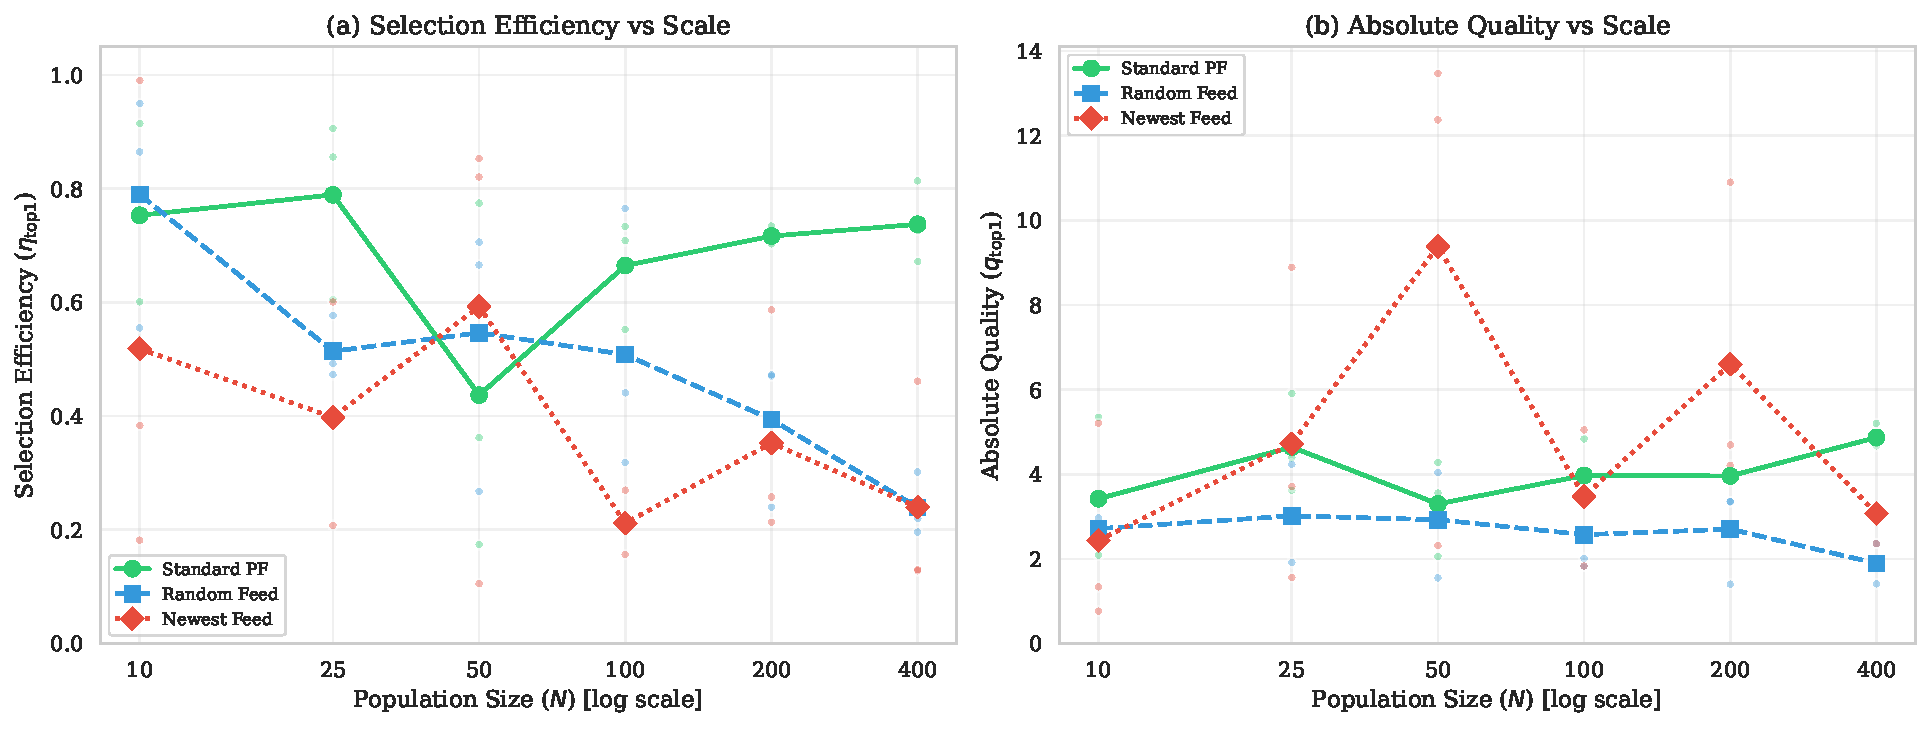
\includegraphics[width=\textwidth]{figures/plot_1_agenda_control_scaling.pdf}
\caption{Scaling trajectory of Synesis. PersonalFocus maintains high selection efficiency at $N=400$ despite a non-monotonic trajectory, with high seed-level variance at intermediate scales ($\eta = 0.44$ at $N=50$). The mechanism recovers at larger $N$. Absolute quality was constrained by DAG depth, which decreased at high $N$ due to the fixed 30-day simulation window.}
\label{fig:scaling}
\end{figure}

\paragraph{What the simulation does \textit{not} confirm.}
The absolute quality ceiling did not increase monotonically with $N$ in these experiments, because DAG depth (the mechanism through which quality accumulates) was constrained by the fixed time window. Realizing the full $\log(Nn)$ scaling at large $N$ requires either proportionally longer deliberation windows or topology-aware routing that channels attention toward deepening existing lineages rather than initiating new ones (Chapter~\ref{ch:discussion}). The simulation demonstrates that the \textit{selection machinery} scales. Whether the \textit{quality-generation process} scales requires further investigation.

\begin{figure}[ht]
\centering
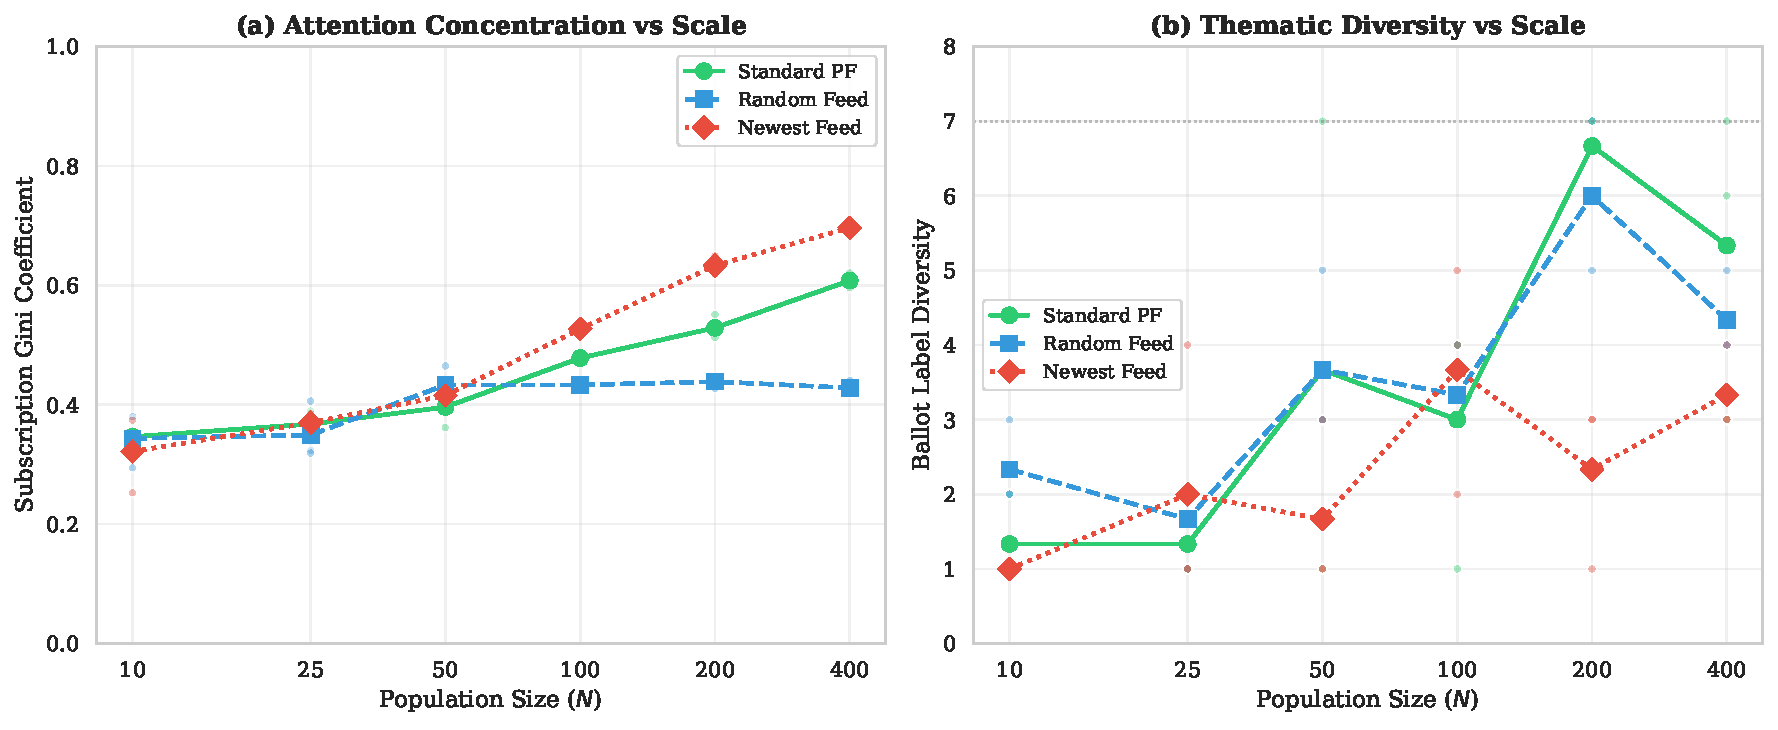
\includegraphics[width=\textwidth]{figures/plot_8_scaling_matrix.pdf}
\caption{Attention concentration and ballot diversity across scales. PersonalFocus deliberately concentrates attention (higher Gini coefficient) to ensure promising proposals receive sufficient evaluation depth.}
\label{fig:scaling-matrix}
\end{figure}


\subsection{Three-Window Architecture Ablation}
\label{sec:sim-three-window}

The Three-Window Architecture (Section~\ref{sec:three-window}) structures collective attention through two independently operable mechanisms: PersonalFocus feed routing (Discovery Window) and the label-exclusive ballot (Collective Window). The \texttt{three\_window} study (24~runs) crosses these in a $2 \times 2$ factorial at $N=50$ and $N=100$.

\begin{table}[ht]
\centering
\caption{Three-Window Architecture $2 \times 2$ factorial ablation (means across 3 seeds per cell).}
\label{tab:three-window}
\small
\begin{tabular}{l c c c c}
\toprule
\textbf{Configuration} & \multicolumn{2}{c}{$N=50$} & \multicolumn{2}{c}{$N=100$} \\
\cmidrule(lr){2-3}\cmidrule(lr){4-5}
 & $\eta_{\text{top1}}$ & $q_{\text{top1}}$ & $\eta_{\text{top1}}$ & $q_{\text{top1}}$ \\
\midrule
Full Platform (PF + Ballot Diversity)       & \textbf{0.870} & 6.88 & 0.811 & 3.88 \\
No Ballot Diversity (PF only)               & 0.621 & 3.62 & 0.744 & 4.88 \\
No Feed Routing (Random + Ballot Diversity) & 0.637 & 3.19 & 0.474 & 2.80 \\
Neither (Random + unconstrained)            & 0.679 & 3.78 & 0.689 & 4.00 \\
\bottomrule
\end{tabular}
\end{table}

Two findings emerge from the factorial design:

\paragraph{Feed routing matters more than ballot diversity.} At $N=100$, removing PersonalFocus reduces selection efficiency by up to 42\% (Full Platform $\eta = 0.811$ vs No Feed Routing $\eta = 0.474$), while removing ballot diversity alone has a much smaller effect ($\eta = 0.811$ vs $\eta = 0.744$). This confirms that intelligent attention routing is the primary driver of selection quality; ballot diversity provides a secondary thematic-coverage guarantee.

\paragraph{Ballot diversity helps at small $N$, costs at large $N$.} At $N=50$, the Full Platform ($\eta = 0.870$) substantially outperforms the No Ballot Diversity variant ($\eta = 0.621$). At $N=100$, the relationship partially reverses: the No Ballot Diversity variant achieves higher absolute quality ($q = 4.88$) than the Full Platform ($q = 3.88$). Between $N=50$ and $N=100$, the ballot diversity cost increased from $\Delta\eta = -0.249$ to $\Delta\eta = -0.067$ (where negative values indicate the Full Platform outperforming the No Ballot Diversity variant). Extrapolation beyond $N=100$ requires additional simulation runs. The root cause is cascading label exclusion: remixed proposals inherit parent labels, so deep-DAG proposals accumulate many labels, blocking high-quality siblings from ballot slots via the any-overlap exclusion rule. A label-weighted scoring mechanism, penalizing overlap proportionally rather than applying hard exclusion, could preserve diversity at lower cost and is a concrete target for future refinement.

\begin{figure}[htbp]
\centering
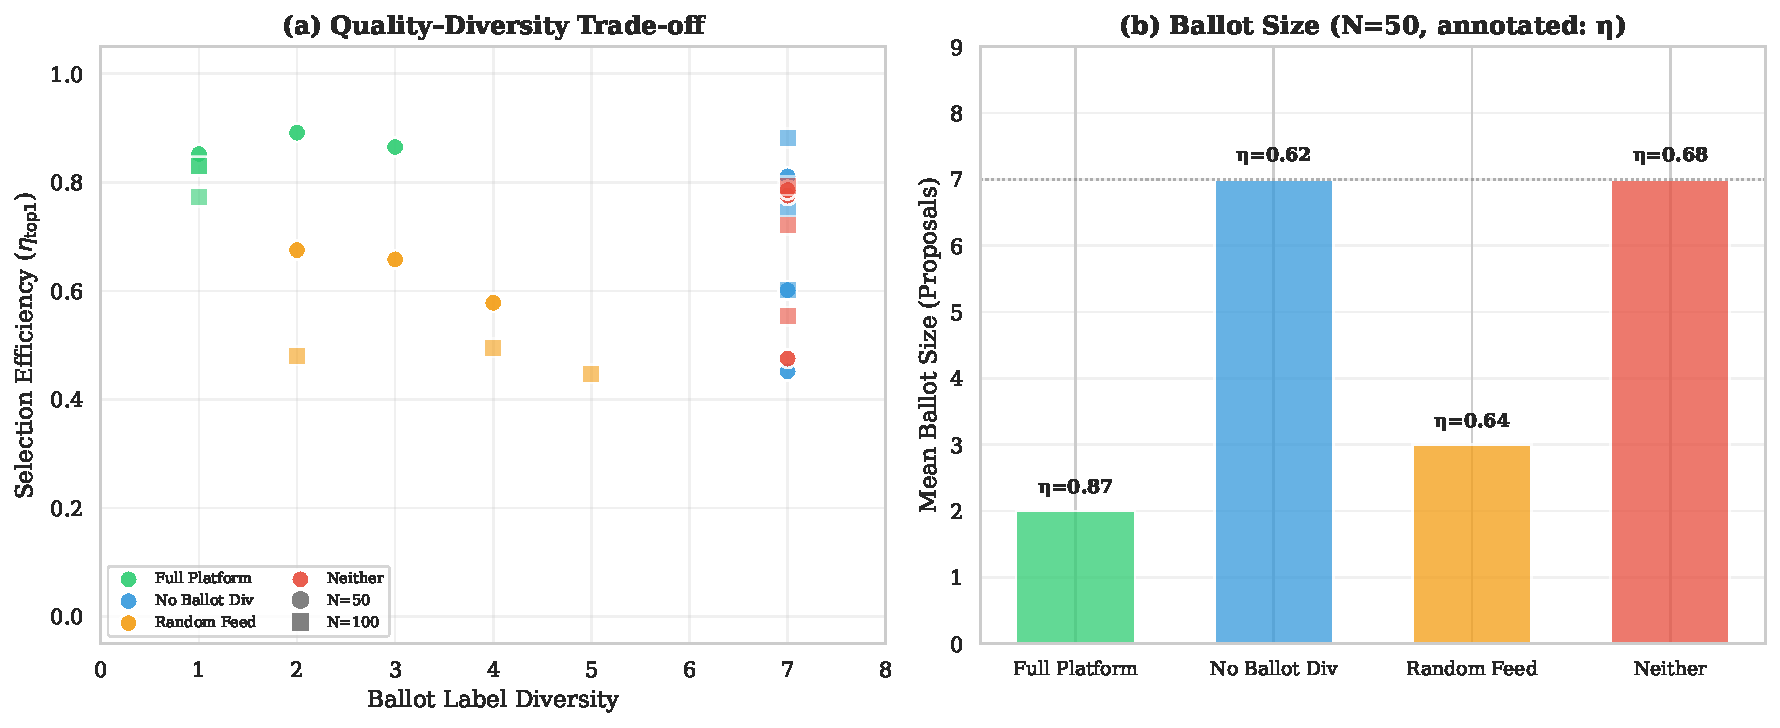
\includegraphics[width=\textwidth]{figures/plot_3_three_window_tradeoff.pdf}
\caption{Three-Window Architecture $2 \times 2$ factorial ablation at $N=50$ and $N=100$. Left: selection efficiency $\eta_{\text{top1}}$. Right: absolute winner quality $q_{\text{top1}}$. The Full Platform achieves the highest efficiency at both scales, but the No Ballot Diversity variant achieves higher absolute quality at $N=100$ due to the ballot diversity cost.}
\label{fig:three-window-ablation}
\end{figure}

\subsection{Attention Coverage Across Feed Regimes}
\label{sec:attention-coverage}

Table~\ref{tab:attention-coverage} reports attention coverage percentage for the final proposal set at two levels: \textit{never interacted} (no \texttt{vote\_support} or \texttt{vote\_migrate} received) and the stricter \textit{never subscribed} (no \texttt{vote\_support}).


\begin{table}[ht]
\centering
\caption{Attention coverage by feed regime and group size. \textit{Never interacted}: no \texttt{vote\_support} or \texttt{vote\_migrate} received. \textit{Never subscribed}: no \texttt{vote\_support} received. The gap between metrics reflects the Siphon Effect's reach beyond direct subscriptions.}
\label{tab:attention-coverage}
\small
\begin{tabular}{l l r r r r r}
\toprule
\textbf{Regime} & \textbf{Metric} & $N=10$ & $N=50$ & $N=100$ & $N=200$ & $N=400$ \\
\midrule
\multirow{2}{*}{PersonalFocus} & Never interacted & 13\% & 14\% & 22\% & 21\% & 36\% \\
 & Never subscribed & 17\% & 22\% & 45\% & 51\% & 80\% \\
\midrule
\multirow{2}{*}{Random Feed} & Never interacted & 30\% & 25\% & 27\% & 23\% & 23\% \\
 & Never subscribed & 39\% & 32\% & 30\% & 27\% & 27\% \\
\midrule
\multirow{2}{*}{Newest Feed} & Never interacted & 20\% & 29\% & 44\% & 57\% & 66\% \\
 & Never subscribed & 23\% & 30\% & 52\% & 72\% & 86\% \\
\bottomrule
\end{tabular}
\end{table}

The gap between the two metrics is most striking for PersonalFocus: at $N=400$, only 36\% of proposals are truly untouched (never interacted), but 80\% never receive a direct subscription. The 44-percentage-point gap consists of proposals reached only by Siphon migrations. PersonalFocus does not make proposals invisible; it makes them visible but unselected; agents evaluate them and choose not to subscribe. Random Feed distributes votes uniformly (never-interacted stable at 23--30\% regardless of $N$) but cannot select quality ($\eta = 0.239$ at $N=400$). Newest Feed achieves the worst coverage at scale (66\% never-interacted at $N=400$) because recency bias concentrates attention on the latest proposals only.


\section{Topological Results: The Shape of Deliberation} 
\label{sec:topological-results}

The DAG structures produced by each study group reveal three distinct topological regimes, summarized in Table~\ref{tab:dag-topology}.

\begin{table}[htbp]
\centering
\caption{DAG topology metrics per study and question. Fork:Combine ratio is the number of single-parent edits divided by multi-parent combinations.}
\label{tab:dag-topology}
\begin{tabular}{lccccccc}
\toprule
 & Props. & Roots & Edits & Combos & Max depth & Mean depth & Fork:Combine \\
\midrule
Pilot (3~Qs) & 27 & 13 & 11 & 3 & 2 & 0.70 & 3.67 \\
\midrule
Study~1 & 13 & 10 & 2 & 1 & 1 & 0.23 & 2.00 \\
\midrule
Study~2 Q1 & 8 & 1 & 6 & 1 & 5 & 2.50 & 6.00 \\
\midrule
Study~2 Q2 & 21 & 8 & 7 & 6 & 4 & 1.38 & 1.17 \\
\bottomrule
\end{tabular}
\end{table}

Three distinct topological regimes emerge from these metrics. The Fork:Combine ratio captures the balance between divergent exploration (single-parent edits that branch the solution space) and convergent synthesis (multi-parent combinations that merge ideas). Study~2 Q1's ratio of 6.00 indicates almost pure iterative refinement on a single lineage---one root, six edits, one combine, producing the deepest graph (max depth~5). Study~2 Q2's near-unity ratio of 1.17 reflects a balance between branching and merging, with 6~combinations cross-pollinating ideas across 8~root clusters. Study~1's flat topology (max depth~1, Fork:Combine of 2.00) reveals that iterative deepening failed entirely: participants produced independent proposals without building on each other's work, a social inhibition pattern analyzed in Section~\ref{sec:qualitative-findings}.

Figure~\ref{fig:proposal-velocity} shows the cumulative proposal creation timeline across both community studies, illustrating the bursty, front-loaded authoring pattern characteristic of all deployments.

\begin{figure}[htbp]
\centering
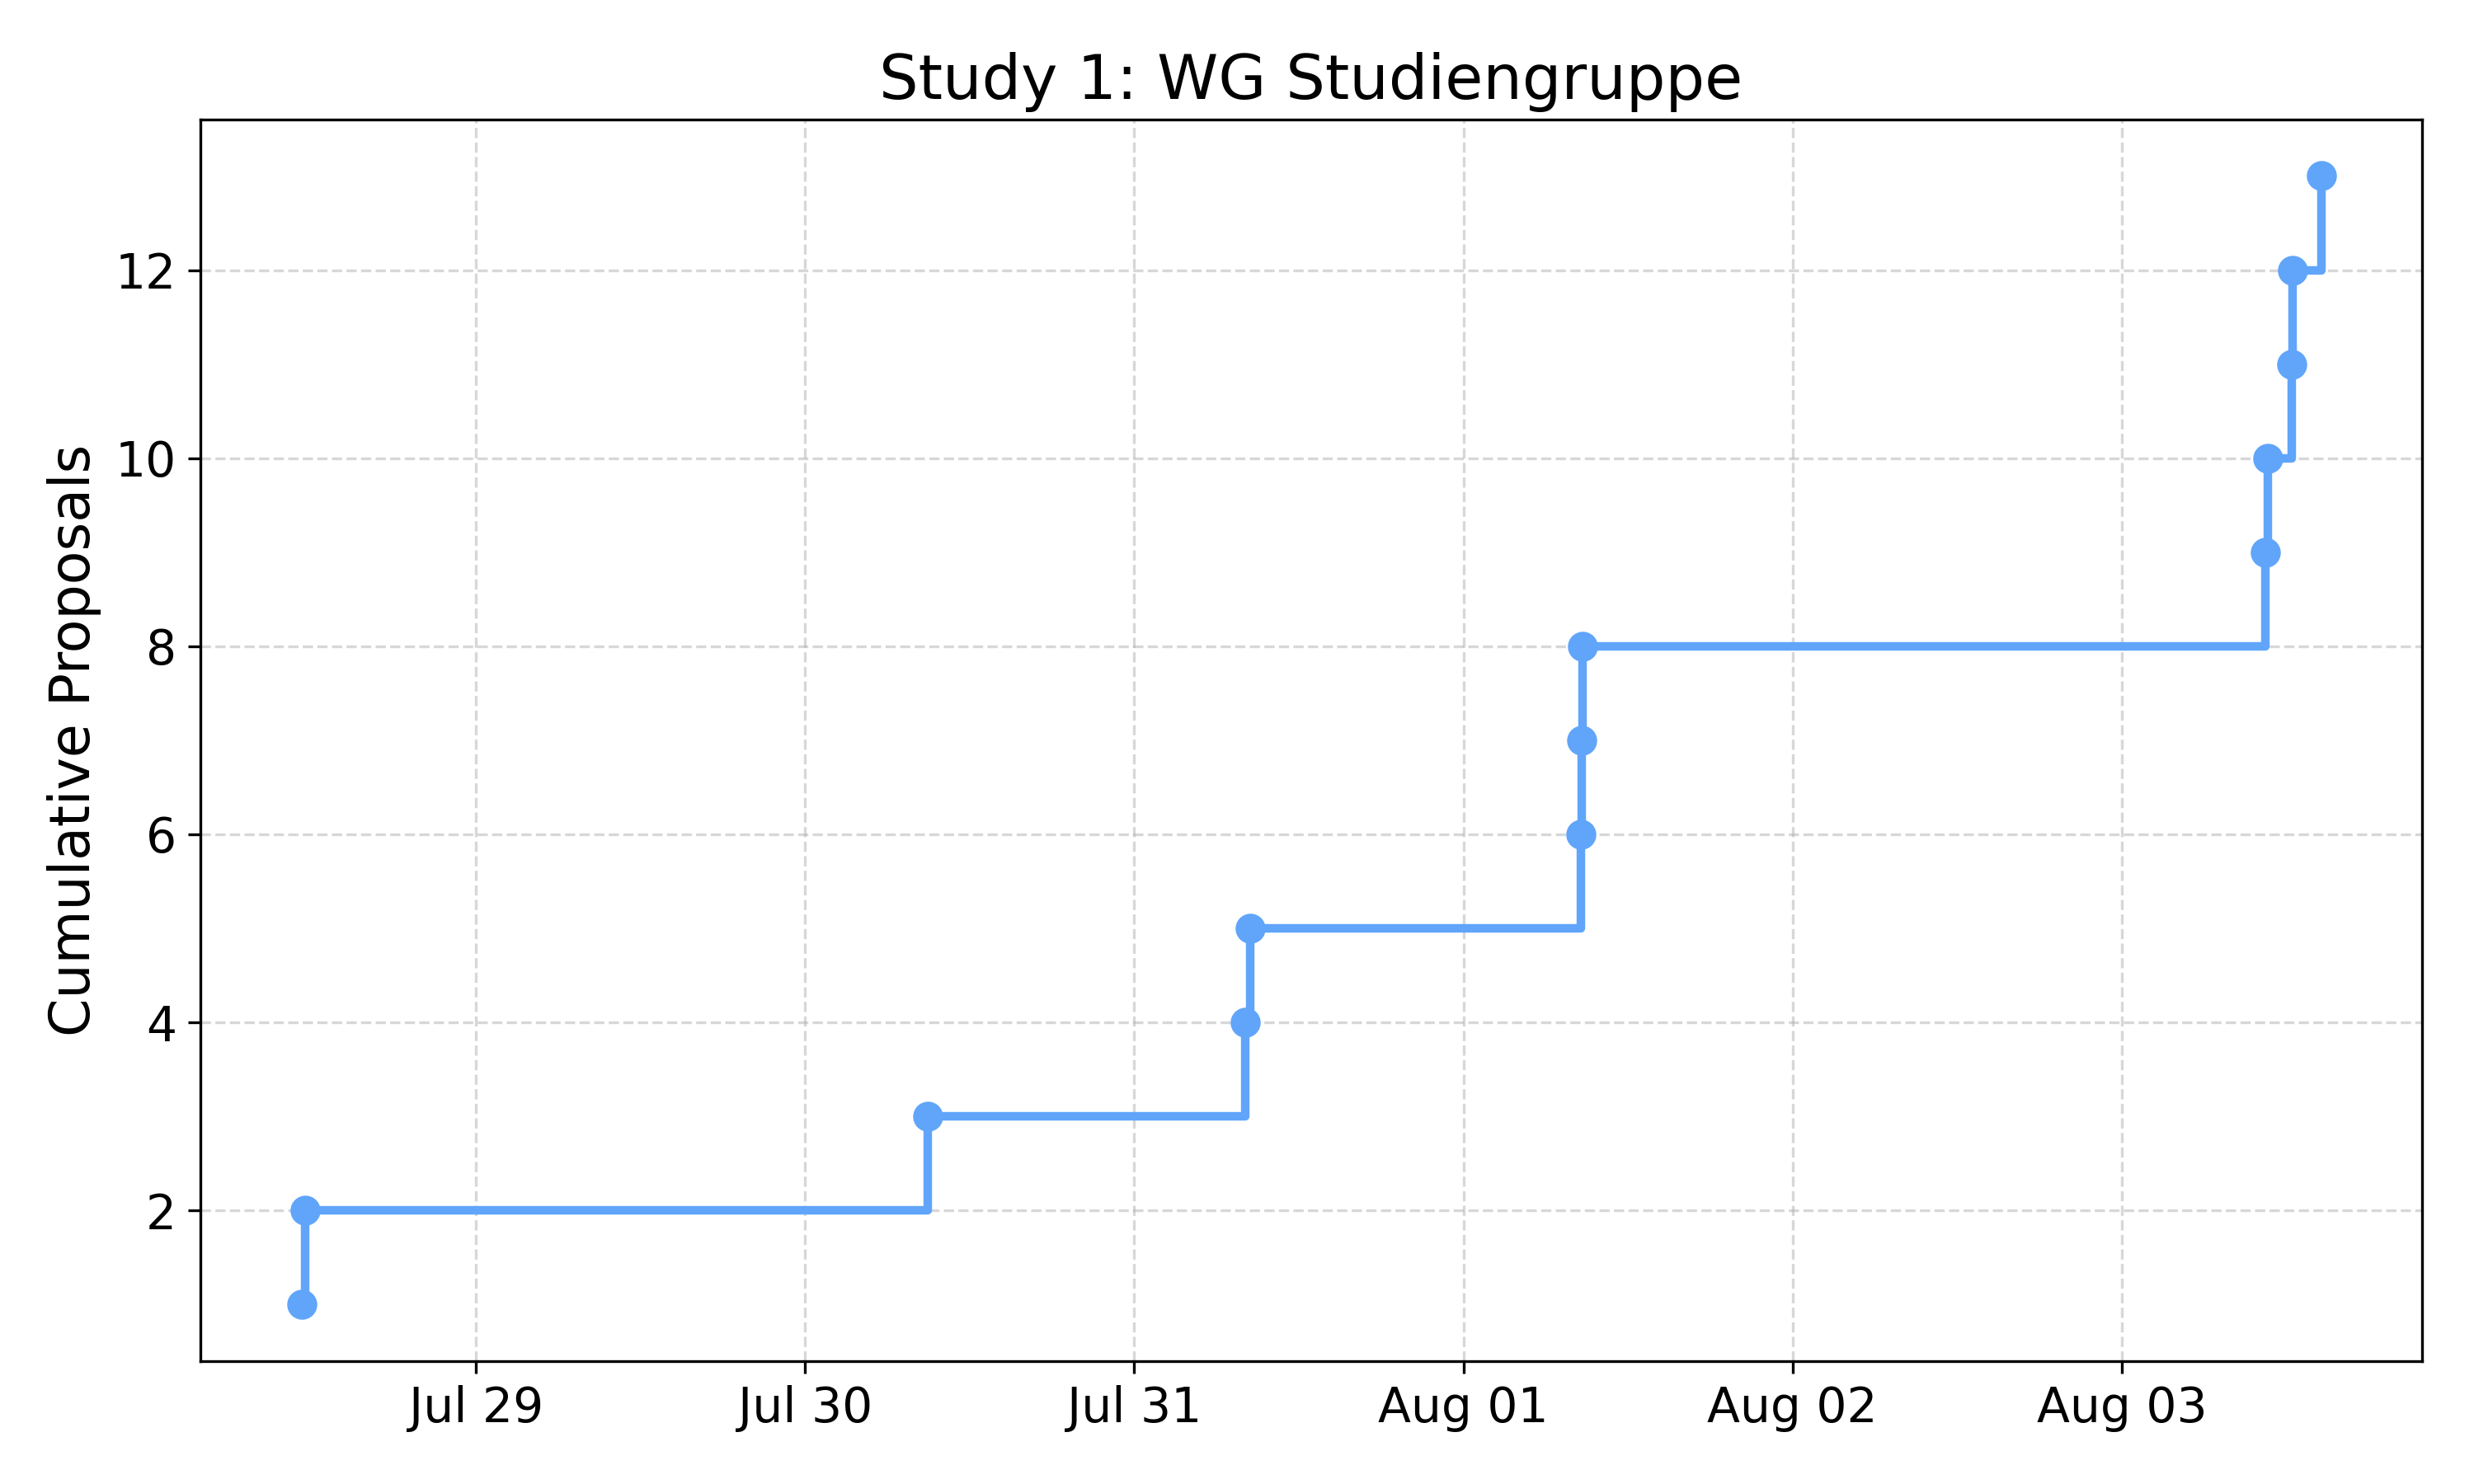
\includegraphics[width=0.9\textwidth]{figures/fig_human_proposal_velocity_0.png}\\[2ex]
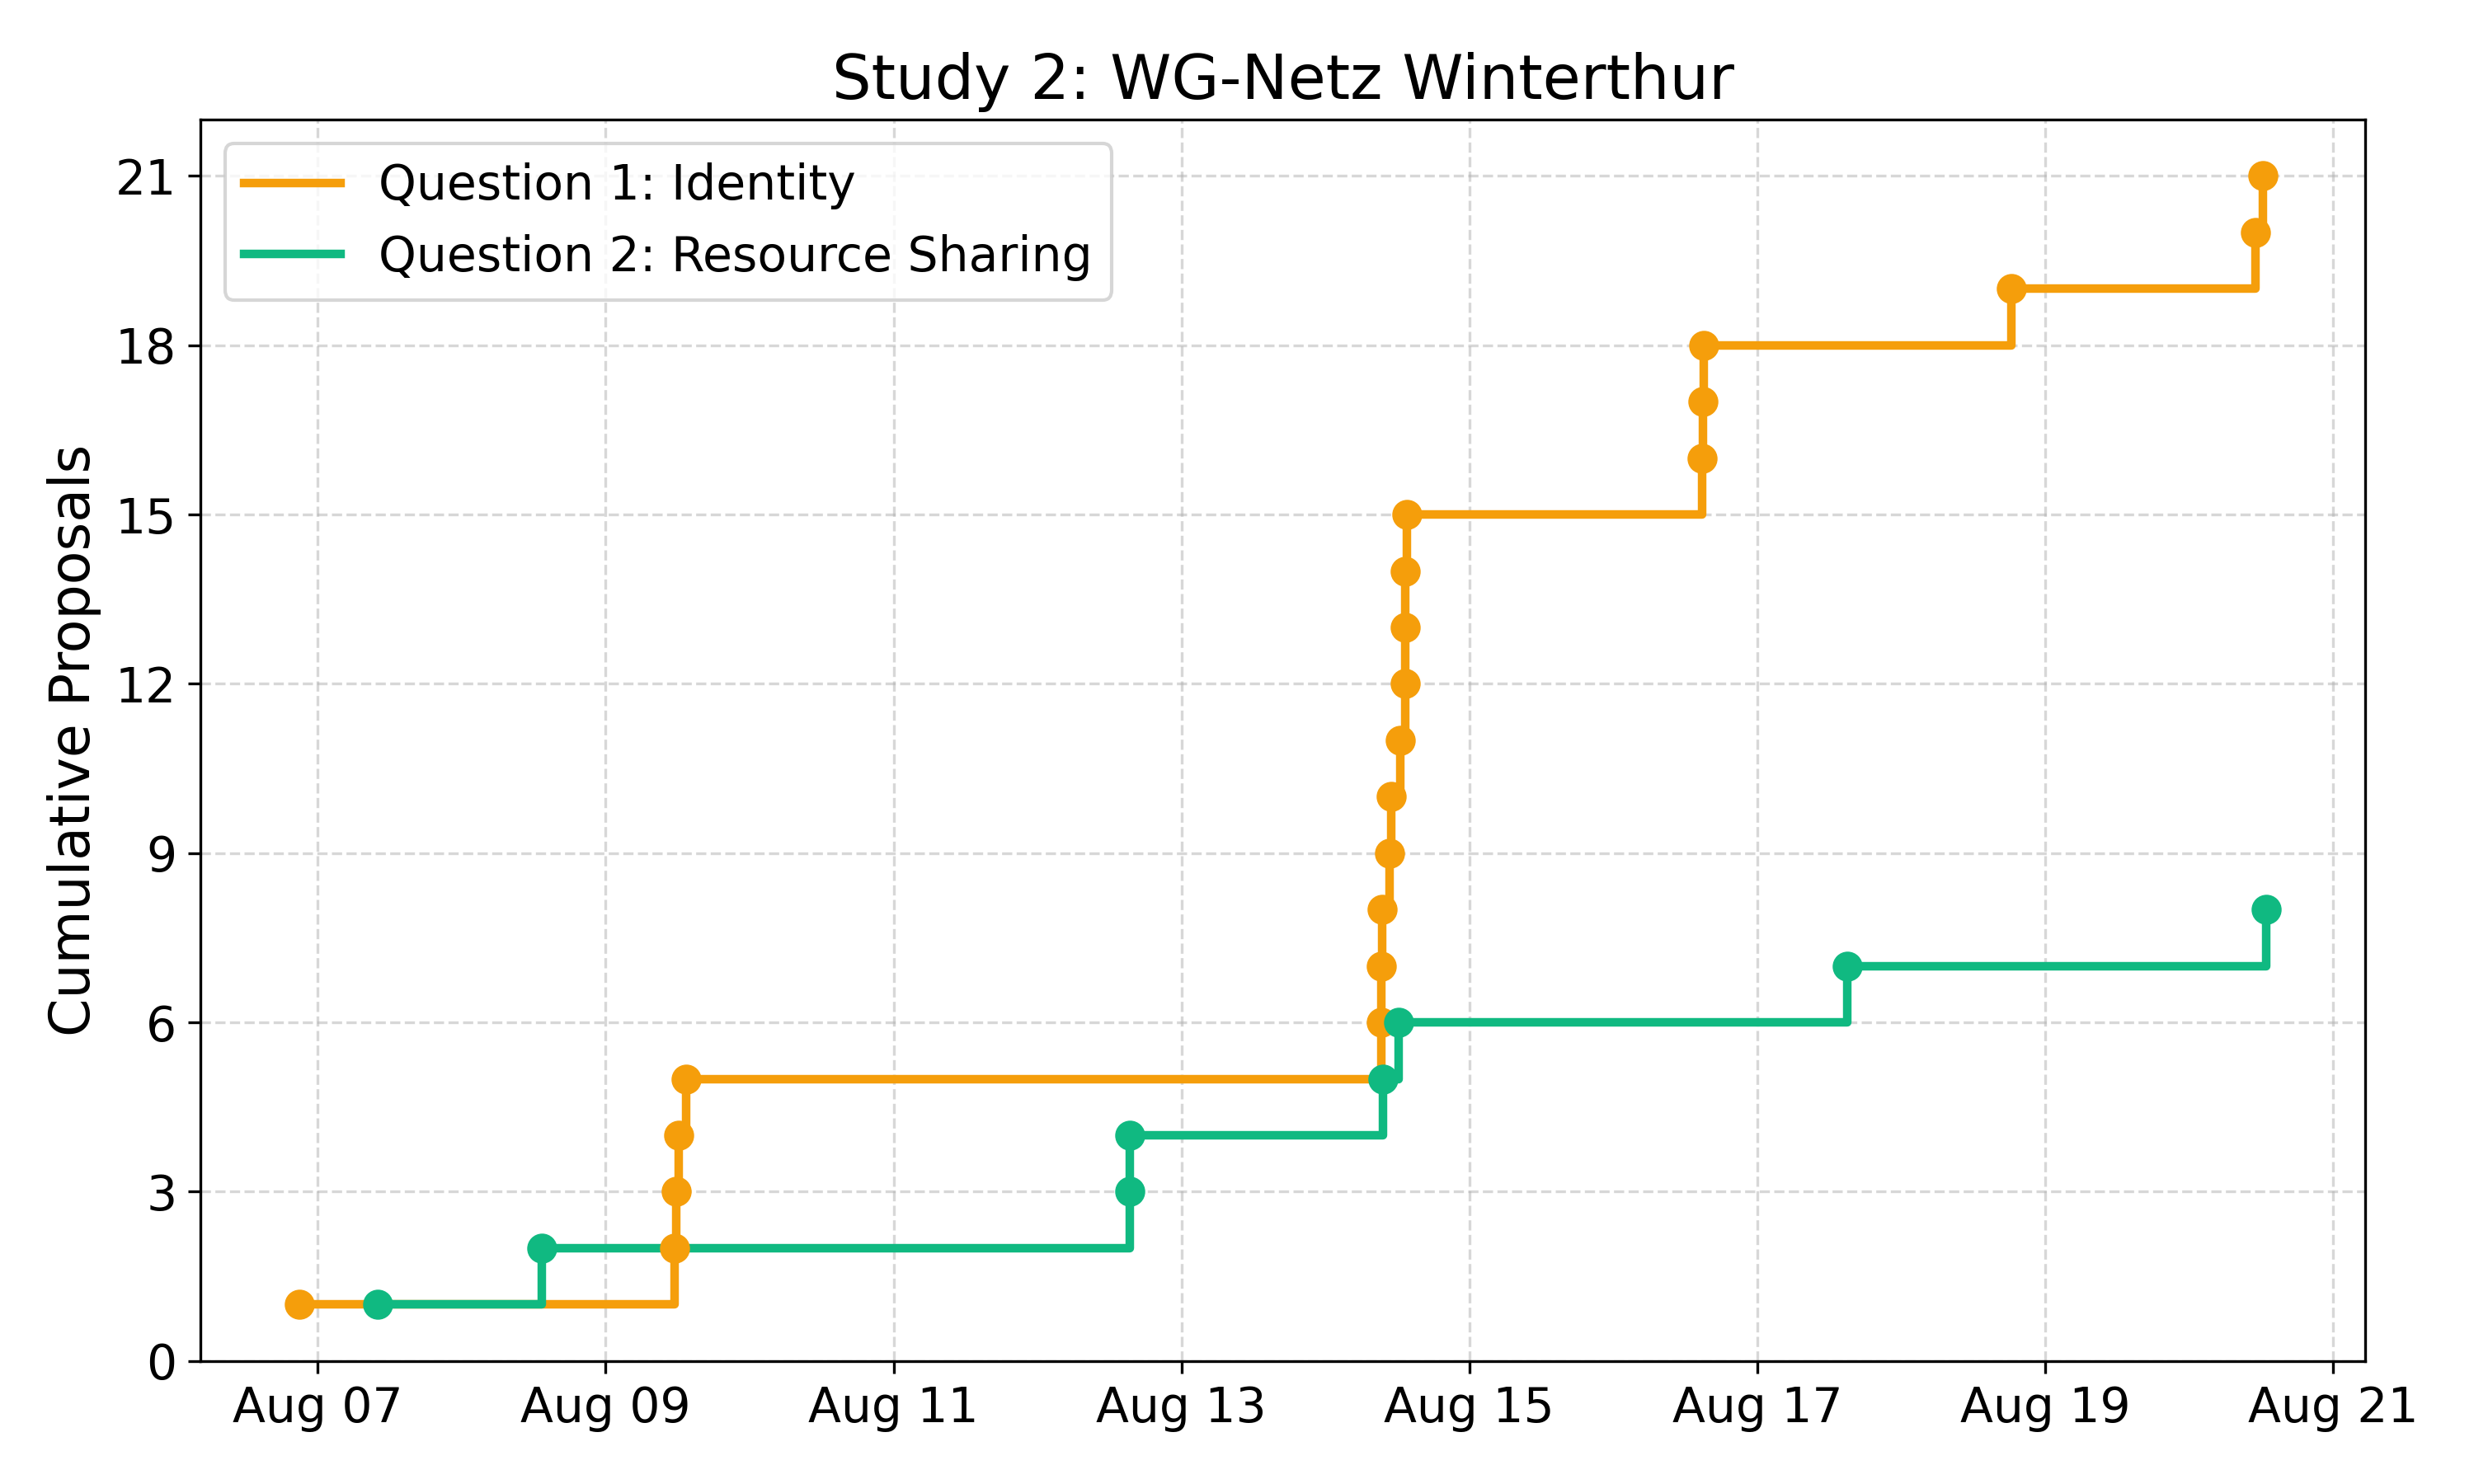
\includegraphics[width=0.9\textwidth]{figures/fig_human_proposal_velocity_1.png}
\caption{Cumulative proposal creation over time for Study~1 (WG Studiengruppe, 12~days)
and Study~2 (WG-Netz Winterthur, 19~days).}
\label{fig:proposal-velocity}
\end{figure}

The topologies ranged from deep iterative refinement to flat independent contributions. Study~2's identity question (Q1) produced a single root proposal iteratively refined through 7~descendants reaching depth~5, with the winning champion at depth~4 after a 10.2-day refinement horizon---demonstrating sustained collaborative improvement. Study~2's resource-sharing question (Q2) generated 8~roots across distinct thematic clusters with 6~combinations indicating cross-pollination: proposals that merged ideas from different thematic branches, departing from the ABM's assumption that proposals compete within a single quality dimension.

The most consequential topology was the \textit{flat landscape} of Study~1: WG-Studiengruppe produced 10~root proposals and only 3~non-root descendants (max depth~1). The survey responses explain this flatness: ``Ich wollte teilweise die Ideen anderer nicht umschreiben, sondern bloss kommentieren, was ich nicht konnte'' (``I sometimes wanted to comment on others' ideas rather than rewrite them, which I could not do''). The absence of a commenting mechanism was experienced as a barrier: participants wanted to respond to ideas without rewriting them. This flatness is consistent with the survey finding that participants wanted to comment rather than rewrite (Section~\ref{sec:qualitative-findings}).

Figure~\ref{fig:depth-distribution} shows the branch-depth distribution across all deployments.

\begin{figure}[htbp]
\centering
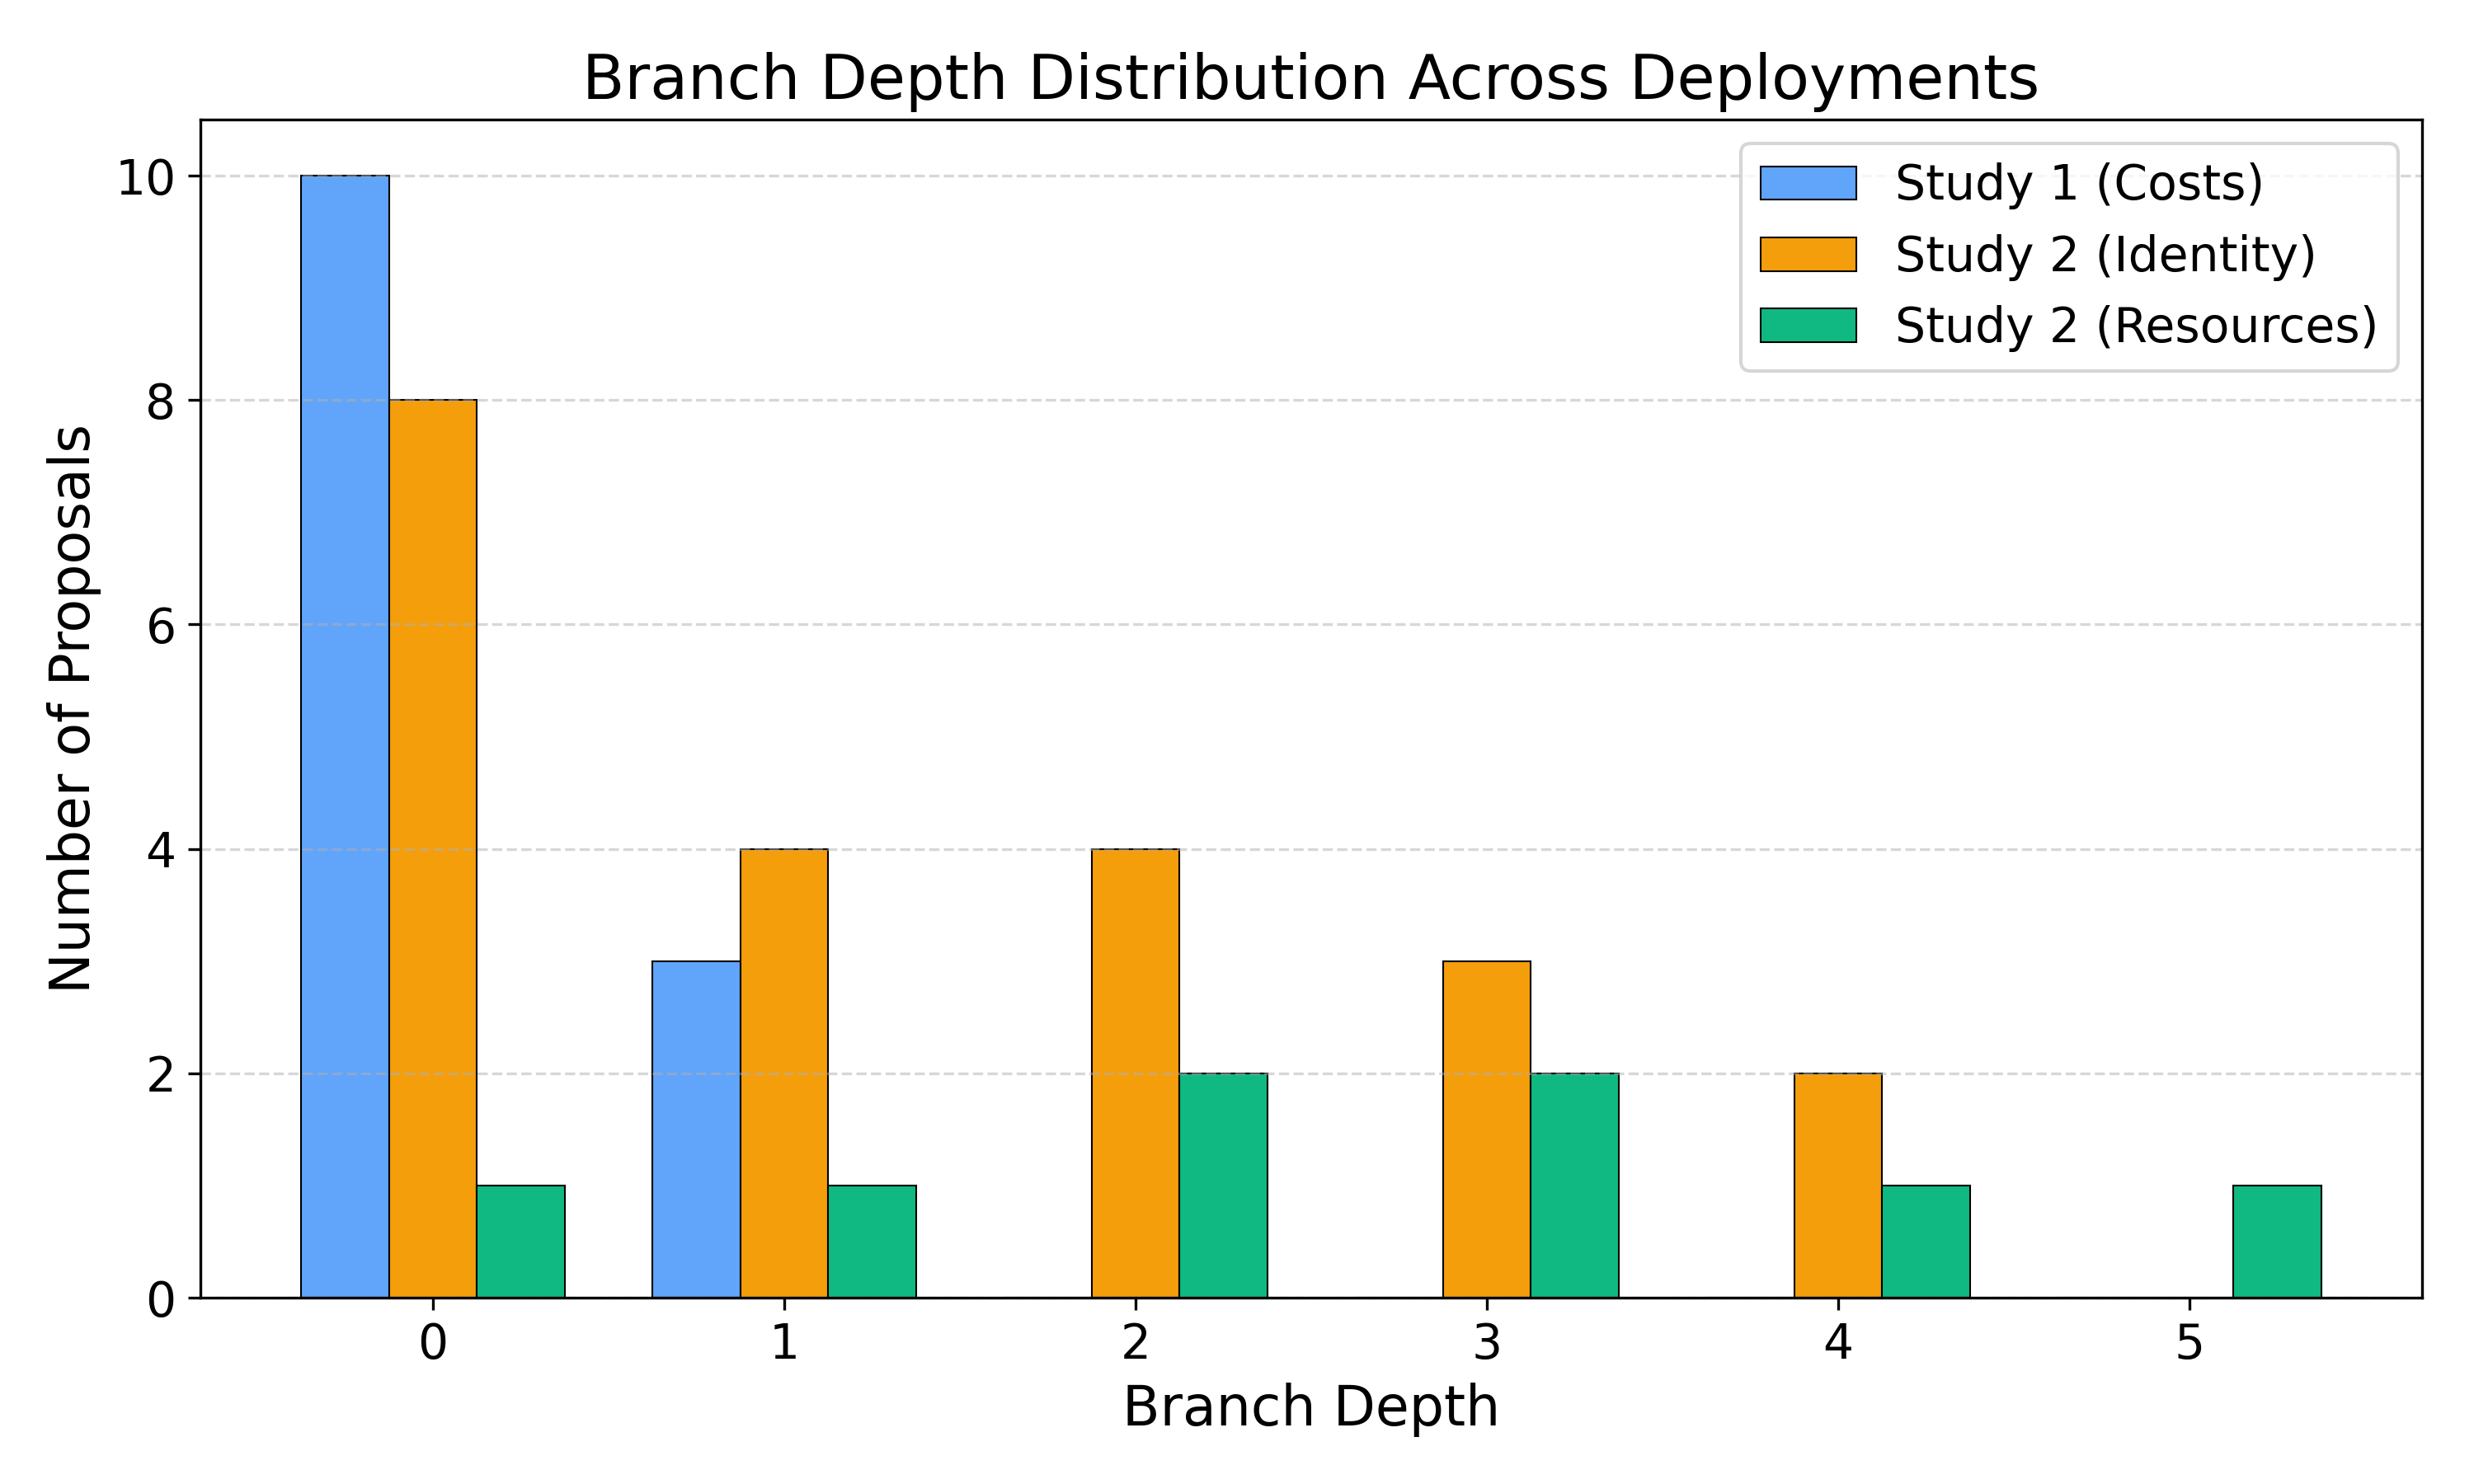
\includegraphics[width=\textwidth]{figures/fig_human_branch_depth.png}
\caption{Branch-depth distribution across all community deployments. Study~2 Q1 produced a single deep refinement chain (maximum depth~5 from one root). In contrast, Study~2 Q2 shows a broader, shallower structure driven by a multi-root exploration pattern (8~roots, max depth~4), and Study~1 remains almost entirely flat.}
\label{fig:depth-distribution}
\end{figure}


\section{Attention Distribution and the Siphon Effect} 
\label{sec:attention-siphon}

\paragraph{Evaluation density.}
Measuring evaluation density as unique viewers per proposal yields substantial coverage: $v = 5.92$ (Study~1) and $v = 6.38$ (Study~2). These values characterize the real engagement budget that asynchronous community participants invest in evaluation. Carpentras et al.\ \cite{carpentras_wisdom_2025} identify $v \approx 50$ evaluations per proposal as sufficient for reliable quality selection under worst-case preference misalignment, though $v \approx 10$ already achieves comparable results with appropriate scoring methods. The observed values fall below even the lower threshold, reflecting the cognitive cost of real deliberation: each evaluation requires reading, comprehending, and comparing proposals, an investment that simulated agents make instantaneously. Despite this, the resulting evaluation coverage fraction (up to 57\% of the theoretical maximum of $n \times \text{proposals}$ in Study~2) indicates that the majority of group members viewed the majority of proposals, ensuring that proposals received sufficient exposure to seed the convergence process.

\paragraph{Siphon Effect and vote migration.}
The trajectory of individual proposal subscriptions, visualized in Figure~\ref{fig:human-subscriptions-per-proposal}, provides direct empirical evidence of the Siphon Effect in action. As new remixes were authored and users re-evaluated their choices, older proposals systematically lost subscriptions (downward steps) while new ones gained them.

The Siphon Effect's notification system operated through two channels: Web Push notifications delivered to the device notification center (requiring PWA installation), and an in-app notification panel visible within the application whenever a user opened it. When a subscribed proposal is remixed, subscribers receive a notification prompting them to compare the original with the new version and re-evaluate their subscription.

The mechanism showed variable activity across deployments, directly reflecting DAG depth. In the Pilot, 6~Siphon notifications were sent; all were dismissed without action. In Study~1, 5~notifications were sent and 2~were responded to (40\%), but the flat DAG (max depth~1) limited the number of parent--child relationships available to trigger migrations. Study~2 produced the strongest Siphon activity: 25~notifications were sent and 14~were responded to (56\%), distributed across 4~distinct users. The in-app notification panel logged 47~opens and 20~clicks across 5~users (4 of whom clicked through) in Study~2, confirming that participants actively engaged with the notification system even without PWA installation. The 10.2-day refinement horizon in Q1 was thus supported by both the Siphon mechanism and an organic parallel channel: the study moderator periodically posted reminders in the group's existing messenger channel.

Figure~\ref{fig:human-activity} plots daily action volume across both community studies, revealing the bursty deadline-driven engagement pattern that systematically diverges from the simulation's uniform session model.

\begin{figure}[htbp]
\centering
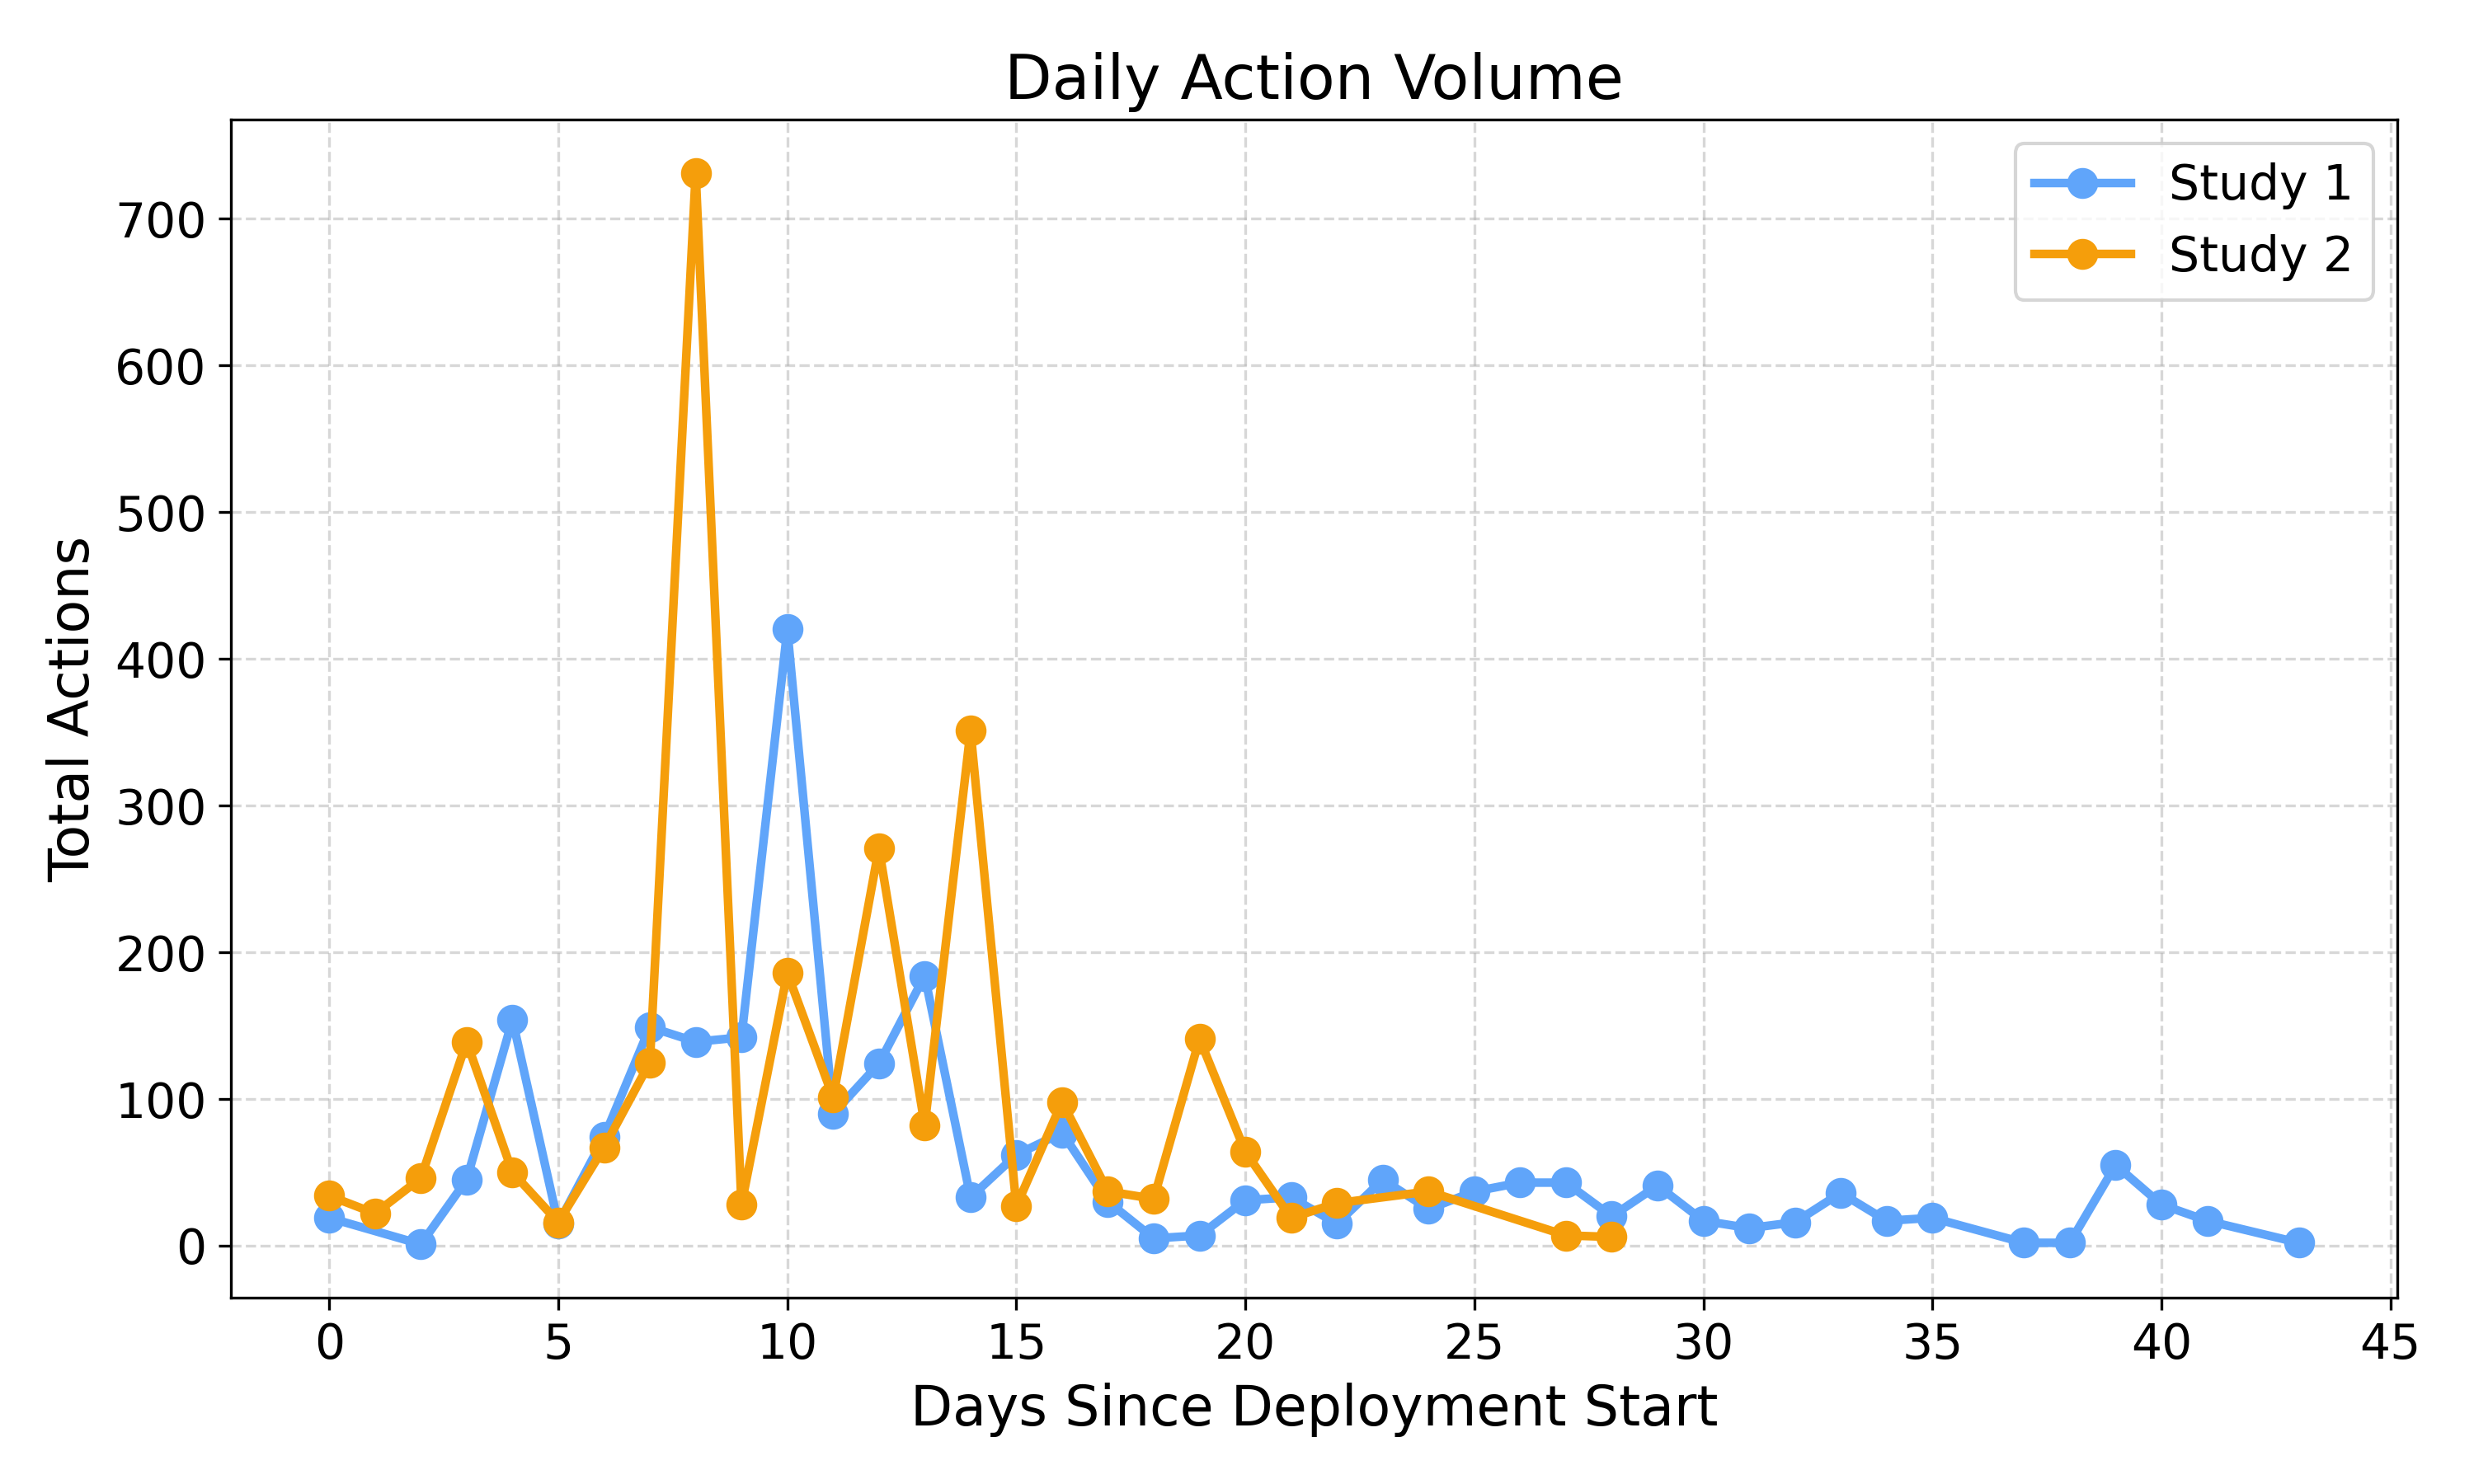
\includegraphics[width=\textwidth]{figures/fig_human_activity_over_time.png}
\caption{Daily action volume across Study~1 (WG Studiengruppe) and Study~2
(WG-Netz Winterthur). Activity concentrates around phase transition deadlines rather
than distributing uniformly, in contrast to the simulation's Poisson-distributed session
model. This bursty engagement pattern is consistent with the heavy-tailed inter-event
time distributions empirically observed in human communication \cite{barabasi2005origin, vazquez2006modeling},
and represents a systematic divergence from agent behavior
documented in Section~\ref{sec:human-divergence}.}
\label{fig:human-activity}
\end{figure}


\begin{figure}[htbp]
\centering
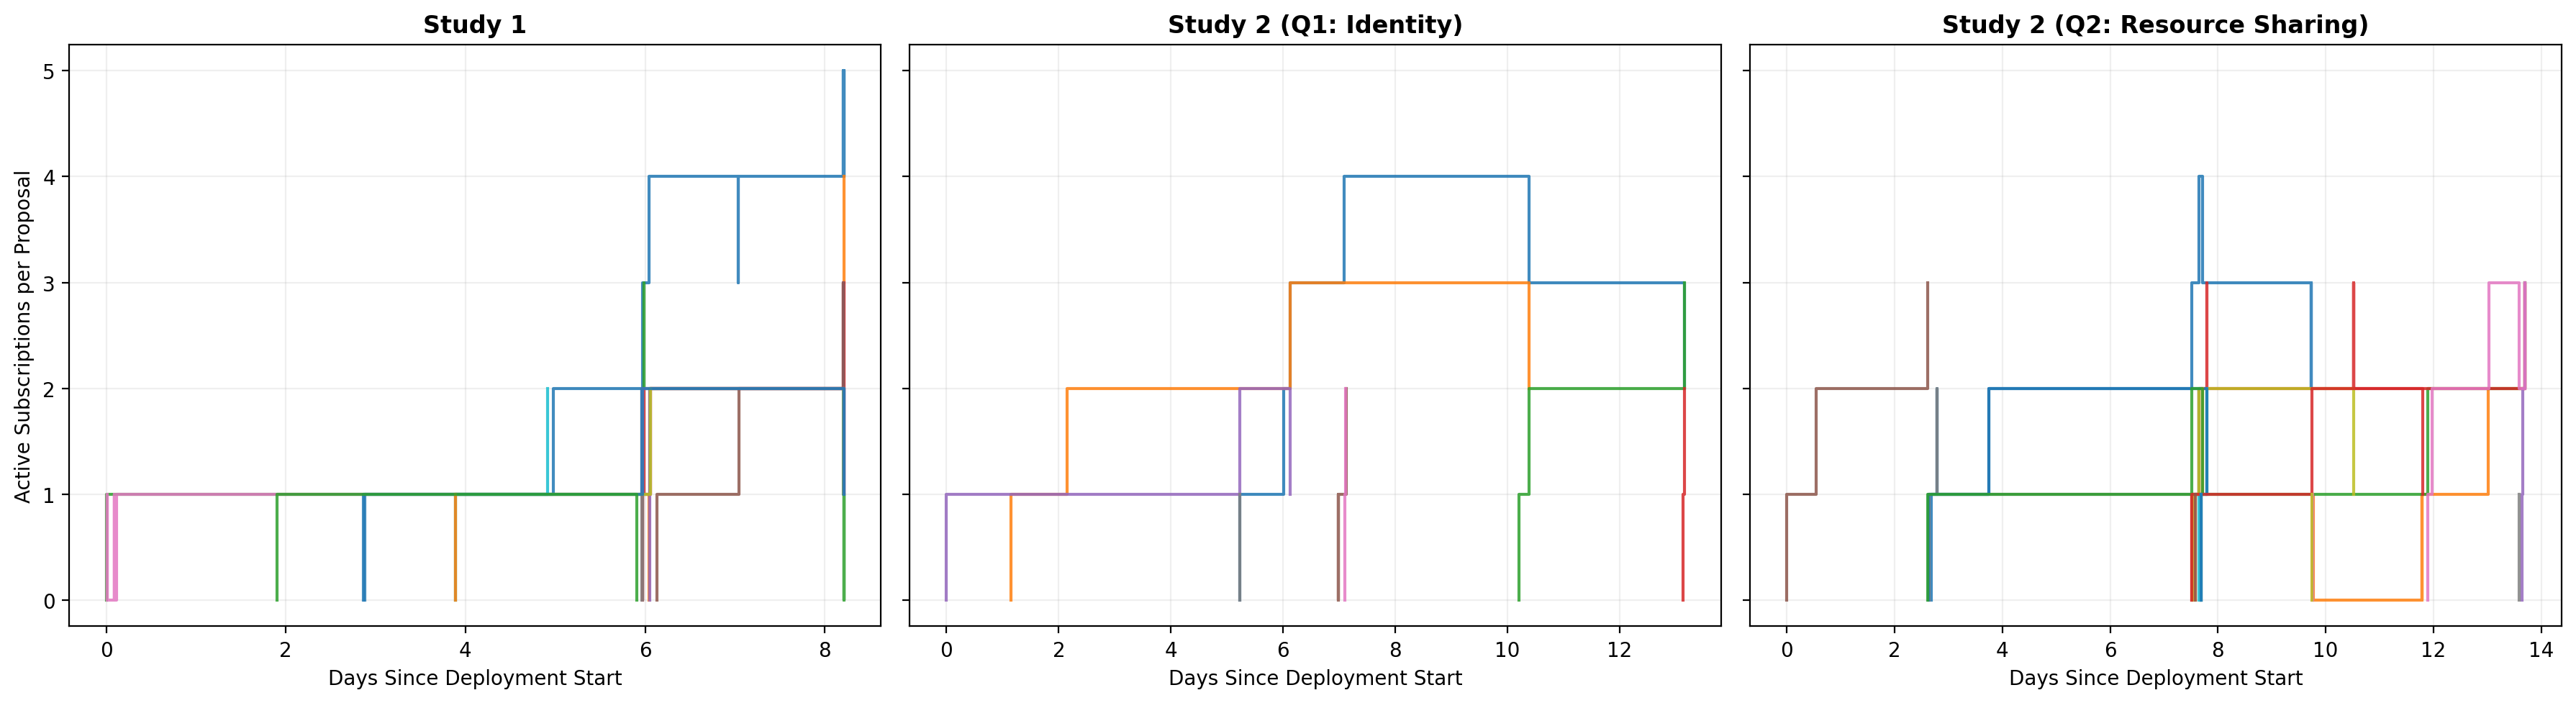
\includegraphics[width=\textwidth]{figures/fig_human_subscriptions_per_proposal.png}
\caption{Active subscription trajectories per individual proposal. This visualizes the Siphon Effect in action: as new remixes are authored and users re-evaluate their choices, older proposals lose subscriptions (downward steps) while new ones gain them.}
\label{fig:human-subscriptions-per-proposal}
\end{figure}

\section{The Interaction Funnel: How Users Engaged} 
\label{sec:interaction-funnel}

\begin{table}[htbp]
\centering
\caption{Engagement funnel across deployments. Each row counts unique consented users who performed the corresponding action type at least once.}
\label{tab:funnel}
\begin{tabular}{lccc}
\toprule
 & Pilot & Study~1 & Study~2 \\
\midrule
Viewed proposals & 6 (86\%) & 11 (100\%) & 12 (100\%) \\
Subscribed & 6 (86\%) & 7 (64\%) & 9 (75\%) \\
Authored proposals & 6 (86\%) & 7 (64\%) & 8 (67\%) \\
Cast ballot & 4 (57\%) & 3 (27\%) & 2 (17\%) \\
\bottomrule
\end{tabular}
\end{table}

The engagement funnel (Table~\ref{tab:funnel}) reveals a consistent pattern: participation drops at each stage of increasing commitment. Two non-consented users in Study~1 and two in Study~2 also viewed proposals but are excluded from all counts. The steepest drop-off in the community studies occurs between viewing and subscribing (Study~1: 100\% $\to$ 64\%), indicating that the transition from passive browsing to active evaluation represents the primary engagement barrier.

\paragraph{User engagement.}
The funnel percentages must be read alongside the absolute engagement each participant invested. In Study~1, users were active on a mean of 6.5~days across the 12-day deployment, generating 194.5~actions per user across a mean of 17.5~sessions per user. In Study~2, users were active on 3.5~of~19~days, generating 135.9~actions per user across 5.4~sessions. Session analysis (using a 30-minute idle-gap threshold) reveals that mean session duration was 8.0~minutes in Study~1 (median: 1.0~min) and 15.0~minutes in Study~2 (median: 5.2~min), with a total mean time investment of 139~minutes per user (Study~1) and 81~minutes per user (Study~2). The high session count and short median duration in Study~1 indicate a pattern of frequent brief check-ins, while Study~2's fewer but longer sessions suggest more sustained engagement per visit. In total, participants invested approximately 2.3~hours (Study~1) and 1.4~hours (Study~2) of active platform time over the deployment period. The deliberation process is not lightweight. Even in a mobile-first, session-distributed architecture, each participant invested substantial sustained attention across multiple return sessions.

\paragraph{Action type composition.}
Platform telemetry reveals that 95--96\% of all logged actions are non-evaluative: page views, tab switches, feed filter changes, session starts, and notification panel interactions. Active evaluative actions (subscribing, unsubscribing, remixing, combining, and ballot submission) constitute only 4--5\% of total actions across all studies. This extreme ratio quantifies the navigation overhead of the platform: users spend the vast majority of their time \textit{reading} and \textit{navigating}, with evaluative output representing a small fraction of total engagement effort.

Figure~\ref{fig:human-action-types} decomposes the full action log by type,
illustrating the extreme skew toward passive navigation relative to active evaluative actions.

\begin{figure}[htbp]
\centering
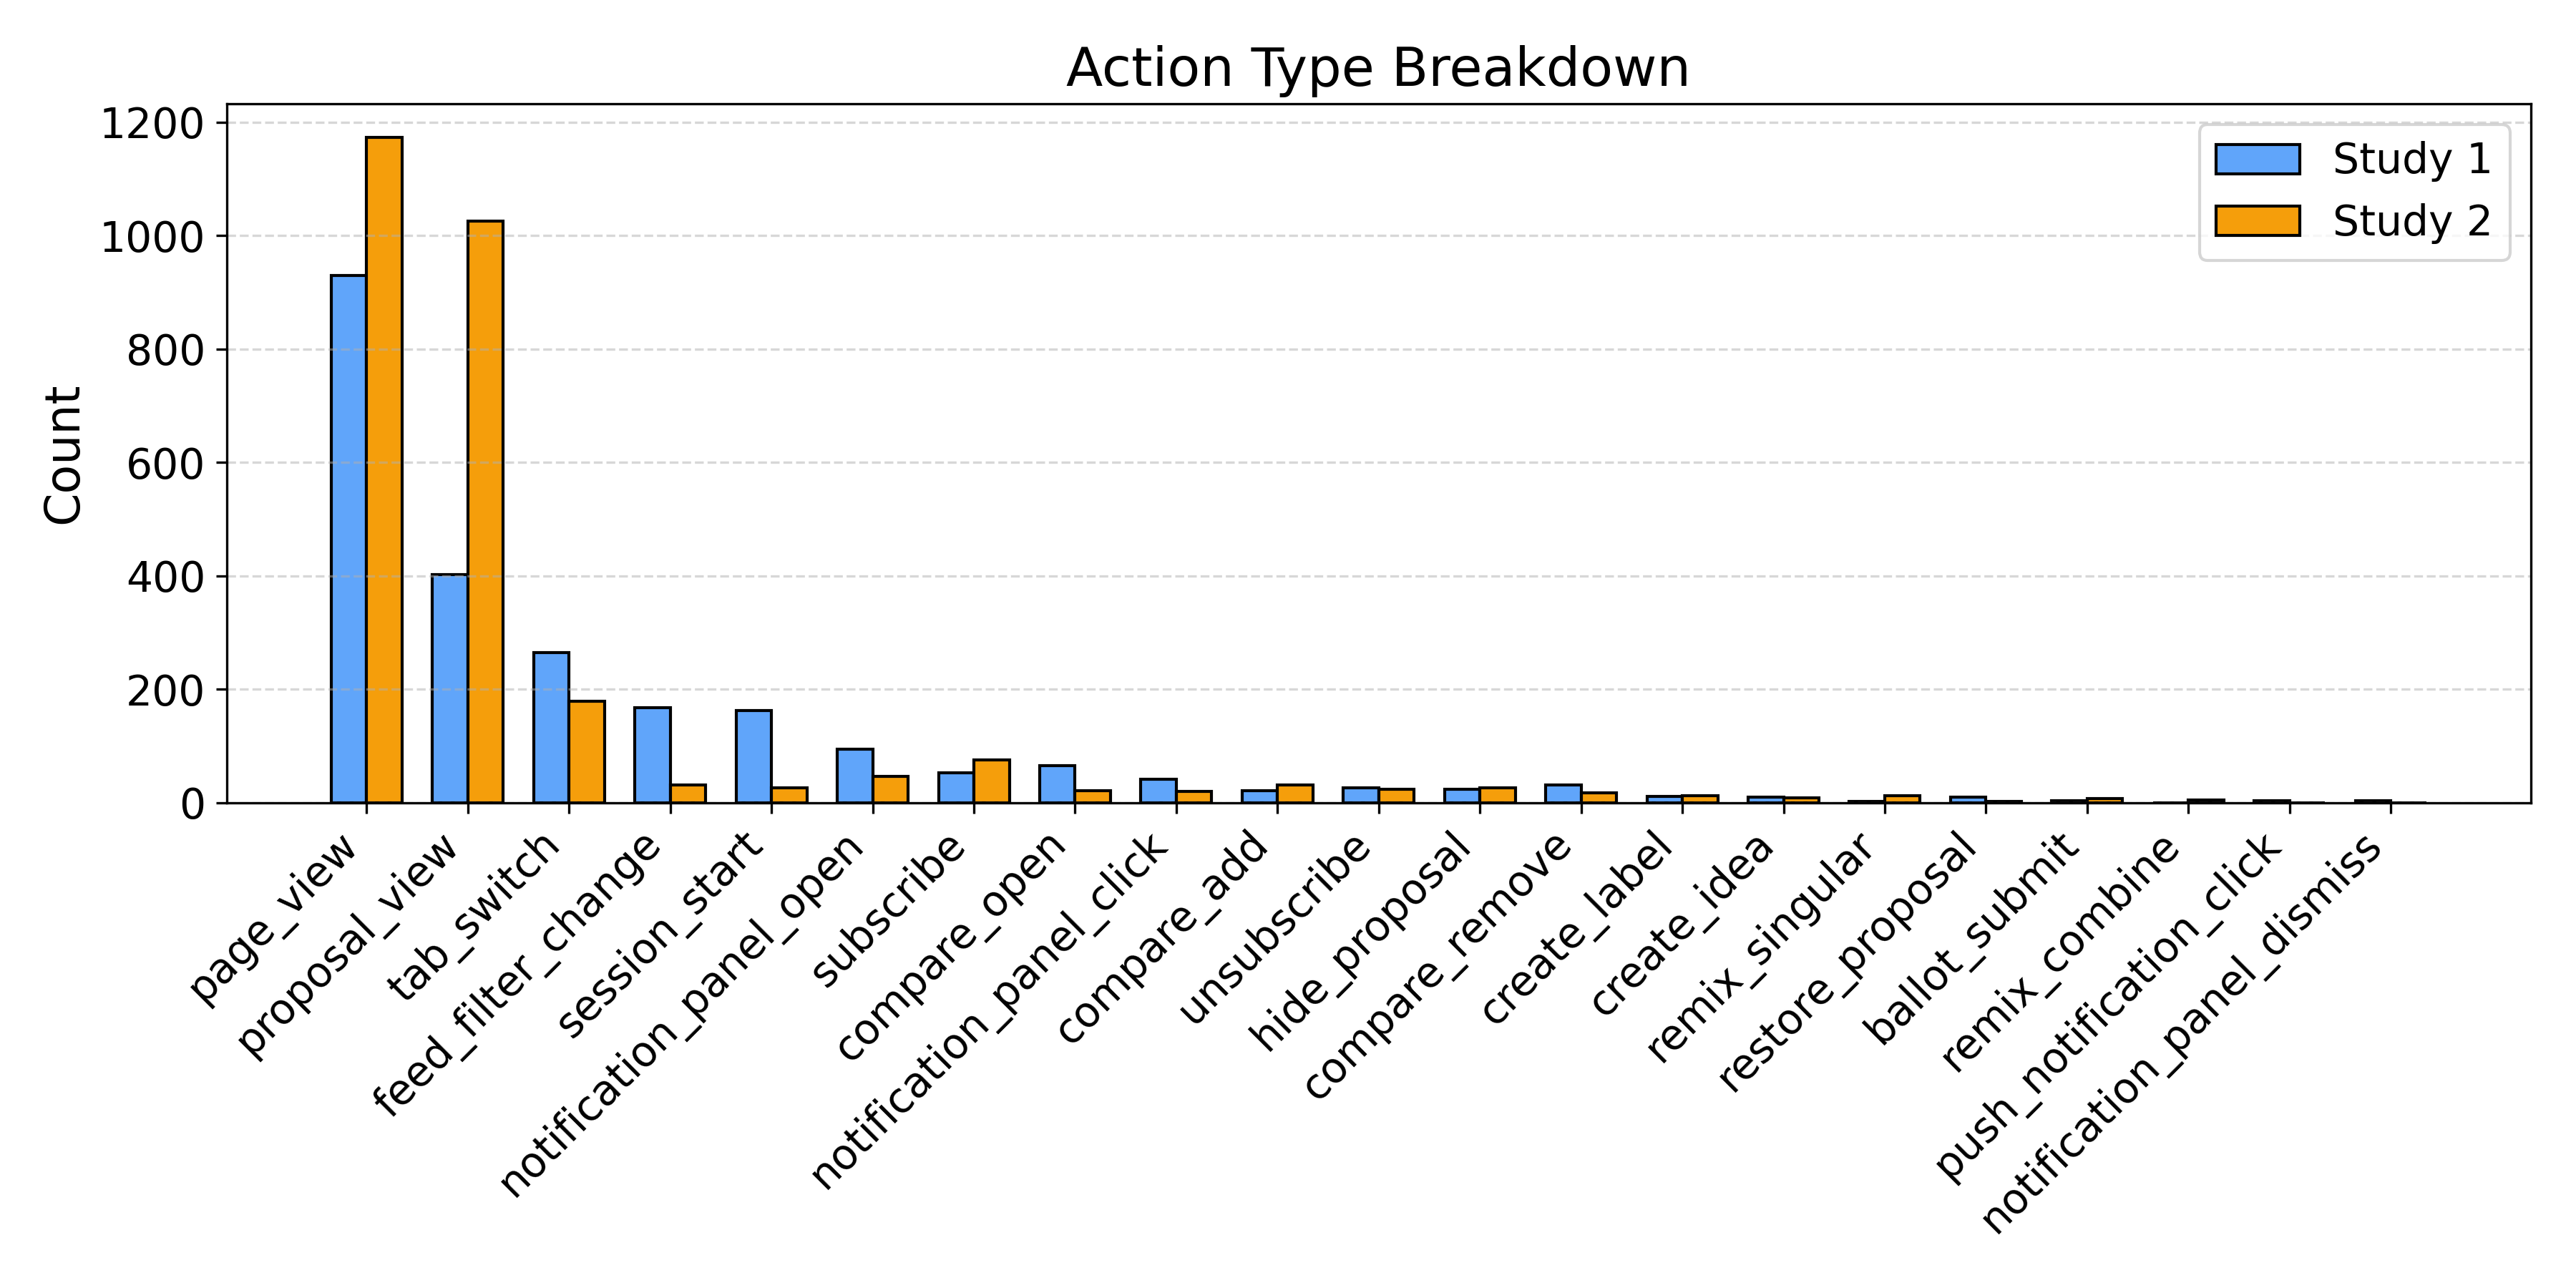
\includegraphics[width=\textwidth]{figures/fig_human_action_types.png}
\caption{Action type breakdown for Study~1 and Study~2. The dominance of passive actions
(page views, tab switches, filter changes) over active evaluative actions (subscribe, remix,
ballot submission) quantifies the cognitive overhead of transitioning from observer to
participant. Evaluative actions constitute 4--5\% of all logged actions across studies.}
\label{fig:human-action-types}
\end{figure}


\section{Qualitative Findings}
\label{sec:qualitative-findings}

Seven participants completed the post-study survey for the two community deployments (4~Study~1, 3~Study~2). The survey included five open-ended questions covering remixing behavior, convergence experience, quality criteria, fairness perceptions, and improvement suggestions. Given the small sample, the following findings are reported as illustrative themes rather than systematic patterns. The formative evaluation's think-aloud observations are not reported as standalone qualitative results; they informed the iterative design refinements documented in Table~\ref{tab:platform-evolution} (Section~\ref{sec:usability-friction}).

\subsection{Remixing Behavior and Motivation}

Participants' experience with remixing varied sharply across deployments. In Study~2, one user described remixing as ``the best feature'' (``Ja das war einfach. Meiner Meinung nach die beste Funktion''). A Pilot participant found the concept ``interesting and useful once you understand the system's mechanics.'' Across both community studies, the remix function was recognized as a distinctive affordance.

However, the absence of a commenting mechanism was a significant barrier. A Study~1 participant reported: ``Ich wollte teilweise die Ideen anderer nicht umschreiben, sondern bloss kommentieren, was ich nicht konnte'' (``I partly wanted to comment on others' ideas rather than rewrite them, which I could not do''). The platform's constrained interaction model requires users to author full proposals rather than leaving lightweight feedback, which created friction with participants' expected communication modes. The implications of this observation are discussed in Section~\ref{sec:embedded-politics}.

Two additional barriers emerged from the survey responses. First, \textit{language difficulty}: finding appropriate formulations for remixes was ``challenging'' (``herausfordernd''), with participants noting that short statements are clearer but risk missing the complexity of the issue. Second, \textit{the two-parent limitation}: the platform restricts combinations to exactly two parent proposals, and participants wished they could ``merge more than 2~ideas at once'' (``mehr als 2~Ideen in einer L\"osung zusammenzubringen'').

\subsection{Convergence Experience}

Participants credited the comparison and remix functions for supporting convergence: ``Unterst\"utzt hat sicher die Vergleichs und Remix-Funktion, sowie die grafische Darstellung'' (``The comparison and remix functions, as well as the graphical display, certainly helped''). The graph visualization was described as partially helpful but confusing at scale, with arrow crossings creating visual clutter in larger DAGs.

A recurring theme was the difficulty of tracking multiple simultaneous threads of discussion: ``Es war schwer wenn mehrere Ideen gleichzeitig besprochen wurden'' (``It was difficult when multiple ideas were being discussed simultaneously''). One Study~2 participant noted that convergence becomes increasingly difficult with more participants and limited time: ``Bei mehr Teilnehmenden zunehmend schwieriger den gemeinsamen Konsens \ldots\ wieder zu vereinen wenn begrenzt Zeit ist'' (``With more participants it becomes increasingly difficult to reunite the common consensus when time is limited'').

In Study~1, convergence was described as inefficient because participants found interaction on the platform generally difficult: ``Nicht sehr effizient, da es allgemein allen ein bisschen schwer fiel auf der Plattform zu interagieren'' (``Not very efficient, since it was generally a bit difficult for everyone to interact on the platform'').

\subsection{Quality Criteria and Selection Logic}

When asked how they decided their rankings during the Final Vote phase, participants' responses revealed predominantly intuitive selection strategies. One Study~2 participant described the process as ``purely intuitive'' (``rein intuitiv''). The responses suggest that the structured ballot mechanism did not fundamentally alter participants' evaluation heuristics: participants relied on personal preference and familiarity rather than systematic comparison.

A Study~2 participant identified a structural constraint on quality assessment: ``Durch die bescheidene Anzahl Teilnehmer*innen standen bei gewissen Fragen wenig Remixes und somit wenig Labels zur Verf\"ugung'' (``Due to the modest number of participants, some questions had few remixes and therefore few labels available''). This observation highlights a bootstrapping problem: the label-exclusive ballot's diversity guarantee requires sufficient thematic breadth, which in turn requires enough proposals to populate multiple label clusters.

\subsection{Perceived Fairness and Legitimacy}

Perceptions of fairness diverged along a revealing axis. One Study~2 participant described the system as ``purely democratic'' (``rein demokratisch'') and noted that ``the more participants, the clearer the picture of consensus.'' Another praised the ranked results display: ``Die aufgeschl\"usselte Rangliste der einzelnen Ideen vermittelte ein gutes Bild \"uber die Meinungen in der Gruppe'' (``The itemised ranking of individual ideas conveyed a good picture of the group's opinions'').

However, a second Study~2 participant identified a structural inequality: ``Es bevorzugt motivierte und engagierte Personen mit technischem Flair. Man muss eine gewisse Startenergie investieren und oft wieder auf die Plattform um an der Diskussion zu bleiben'' (``It favors motivated and engaged people with technical flair. You need to invest a certain start-up energy and return to the platform often to stay in the discussion''). This suggests that the platform's structural neutrality (equal rights for all users) does not guarantee substantive equality of participation when the tool itself demands technical literacy and sustained engagement. The implications of this observation are discussed in Section~\ref{sec:embedded-politics}.

A Study~1 respondent offered a more tempered assessment: ``Mässig fair, da die Schwelle zu hoch ist. In einem professionellen Setting vielleicht anwendbar'' (``Moderately fair, because the threshold is too high. Perhaps applicable in a professional setting''), suggesting that the platform's entry barrier itself undermines perceived fairness regardless of the process's structural neutrality.

In Study~1, one participant questioned fairness not because of the platform's mechanics, but because of uneven participation: ``Ich habe nicht das Gef\"uhl, dass es fair ist, da wir alle zu wenig gewissenhaft mitgemacht haben'' (``I don't feel it was fair, because we all participated too half-heartedly''). This response distinguishes between \textit{procedural} fairness (which the platform provides or not) and \textit{participatory} fairness (which depends on engagement levels that the platform cannot enforce).

\subsection{Usability Friction Points}
\label{sec:usability-friction}

The most consistent improvement request across all studies was better onboarding. A Study~2 participant requested ``a tutorial video,'' a Pilot participant suggested ``a clear, step-by-step tutorial explaining all features,'' and the formative evaluation session (Section~\ref{sec:formative-eval}) identified that the ballot section was never visited without observer prompting.

Technical language was a barrier in the German-language deployments: one Study~1 participant asked whether terms like ``Konvergenz'' and ``Remixen'' could be avoided or replaced with simpler alternatives. Study~2 participants requested ``a leaner design'' (``ein schlankeres Design'') and ``smoother operation'' (``fl\"ussigeres Bedienung'').

In the design-science framework~\cite{hevner2004design}, iterative refinements constitute a core result: each build-evaluate cycle produces design knowledge that shapes the subsequent artifact version. The platform underwent several significant design iterations between evaluation cycles, each traceable to specific findings. Early prototypes used rigid phase loops (all propose, then all vote, then repeat); this was replaced with a continuous asynchronous model at the cost of harder visibility guarantees for late proposals. The full DAG overview was replaced with feed-based listing and local neighborhood views after the formative evaluation revealed cognitive overload among non-technical users. Inline editing was introduced to lower the remixing barrier, and a comparison view was added so users could quickly see what changed between a parent and its remix. The subscribe-equals-endorse signal model collapsed two actions into one during the Discussion phase, simplifying the convergence pipeline. Push notifications were introduced to support the Siphon Effect's dependency on timely alerts. Table~\ref{tab:platform-evolution} summarizes these changes.

\begin{table}[htbp]
\centering
\caption{Platform design changes between evaluation cycles. Each change traces back to a specific finding from the preceding cycle.}
\label{tab:platform-evolution}
\begin{tabularx}{\textwidth}{p{4cm}Xl}
\toprule
Change & Rationale & Source \\
\midrule
Full graph overview removed; local-neighborhood view on detail page & The full graph overview caused cognitive overload, particularly for non-technical users; separating it into localized neighborhood views reduced interaction friction & Formative eval \\
\midrule
Replaced automated clustering with user-generated labels & Cluster membership logic was opaque, preventing users from predicting how proposals would be grouped & Formative eval \\
\midrule
Mobile-first responsive redesign & Majority of community participants expected to use smartphones; pilot confirmed 57\% mobile access & Design decision \\
\midrule
Button placement and inline editing on detail pages & Subscribe button was invisible; combine feature was not discovered & Formative eval \\
\midrule
Enhanced comparison views & Lowered the barrier for evaluating differences between proposals & Pilot feedback \\
\midrule
Push notification system (PWA) & Siphon Effect requires timely notifications for vote migration & Formative eval \\
\bottomrule
\end{tabularx}
\end{table}

\section{Human vs.\ Simulated Attention Patterns}
\label{sec:human-vs-sim}

Table~\ref{tab:human-vs-sim} compares per-user engagement metrics between the human field deployments and simulated runs at comparable group sizes. Simulation agents do not produce view-based evaluations; the comparison therefore focuses on subscription and remix rates. The Siphon column reports notifications sent and responded to for human studies, and atomic \texttt{vote\_migration} actions per run for the simulation.

\begin{table}[ht]
\centering
\caption{Human vs.\ simulated attention patterns. Human data from WG~Studiengruppe ($N=11$) and WG~Netz ($N=12$); simulated data from \texttt{scaling\_frontier} at $N=10$.}
\label{tab:human-vs-sim}
\small
\setlength{\tabcolsep}{5pt}
\begin{tabular}{@{}l r c c c c@{}}
\toprule
\textbf{Study} & $N$ & \textbf{Evaluations/User} & \textbf{Subscriptions/User} & \textbf{Remixes/User} & \textbf{Siphon} \\
\midrule
WG Studiengruppe & 11 & 27.2 & 1.6 & 0.2 & 5\,$\to$\,2 \\
WG Netz Winterthur & 12 & 68.3 & 3.4 & 1.3 & 25\,$\to$\,14 \\
Simulation ($N{=}10$) & 10 & --- & 7.9 & 2.6 & 24.0 \\
\bottomrule
\end{tabular}
\end{table}

Human subscription rates are $2.1$--$4.9\times$ lower than simulated agents, reflecting the cognitive cost of real deliberation: each subscription decision requires reading, comprehending, and comparing proposals rather than instantaneous evaluation. Remix intensity shows a similar pattern, with Study~2 approaching half the simulation rate ($1.3$ vs.\ $2.6$). Siphon activity differs sharply: 2 of 5~notifications were responded to in Study~1 (40\%) and 14 of 25~in Study~2 (56\%), compared to 24.0~atomic migration actions per simulation run. The gap reflects the reduced DAG depth in human studies, which limits the parent--child relationships available to trigger migrations. The simulation therefore represents a \textit{mechanical ceiling}: the performance envelope when all mechanisms operate as designed with full engagement.

\begin{figure}[htbp]
\centering
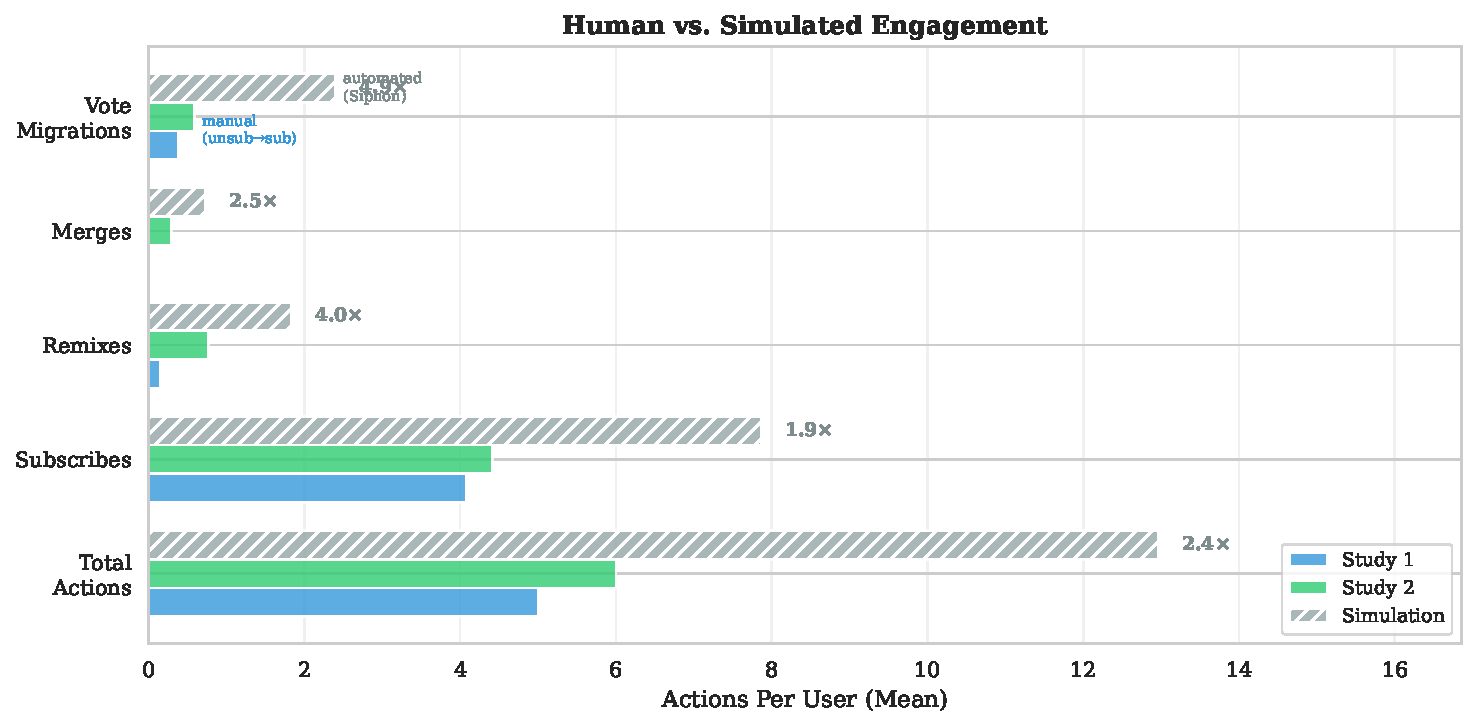
\includegraphics[width=\textwidth]{figures/plot_11_human_vs_sim.pdf}
\caption{Human vs.\ simulated attention patterns. Comparison of action distributions between WG~Studiengruppe, WG~Netz~Winterthur, and simulated runs at $N=10$.}
\label{fig:human-vs-sim}
\end{figure}

\chapter{Summary, Discussion, and Outlook}
\label{ch:discussion}

\section{Summary of Findings}
\label{sec:summary-findings}

This thesis designed, implemented, and evaluated Synesis, a web-based tool that translates the remixing-based collective intelligence model of Carpentras et al.\ \cite{carpentras_empowering_2024, carpentras_wisdom_2025} into a working deliberation system. The platform structures collective attention through a Three-Window Architecture (Discovery, Evaluation, Collective) and implements subscription-migration dynamics through the Siphon Effect. Three deployments, a formative pilot ($n=7$) and two community studies ($n=11$, $n=12$), complemented by agent-based simulation experiments, generated design knowledge about how human behavior departs from the theoretical model's assumptions and how the system's mechanisms scale.

\paragraph{RQ1 (System Design).}
The process of implementing a remixing simulation to user deployment produced five key design findings. First, \textit{asynchronous interaction instead of phased lockstep}: the ABM's rigid phased model (all propose, then all vote) was replaced early in development with a continuous asynchronous model. This was motivated by the impracticality of synchronizing all participants every few days just to progress. The downside to this: The system explicitly needs to handle late entrant proposals.

Second, \textit{balanced views of the shared knowledge base} replaced the ABM's assumption of global visibility. The Three-Window Architecture separates individual exploration (Discovery), personal evaluation (Evaluation), and collective aggregation (Collective). The PersonalFocus heuristic routes each user's attention across the proposal space, balancing individual interests against system-level diversity, though its calibration remains heuristic rather than empirically validated. The full DAG overview was replaced with feed-based listing and local neighborhood views after formative evaluation revealed that non-technical users could not parse the full graph.

Third, \textit{user-generated labels} structure the multi-dimensional proposal space into thematic clusters, enabling the system to surface the best solution per perspective rather than collapsing all proposals into a single ranking. The label-exclusive ballot algorithm assembles the final vote from distinct thematic groups, ensuring that the collective decision reflects the full breadth of approaches rather than the single most popular one.


Fourth, \textit{exploiting the DAG structure} for more efficient proposal evaluations. Because proposals are structurally related, their iterations can be evaluated more easily by people who have already worked with a previous version. This is operationalized using the Siphon Effect, which drove vote re-evaluation through targeted notifications. Siphon activity scaled with DAG depth: Study~2 produced 25~notifications with 14~responded to (56\%), while Study~1's flat DAG generated only 5~notifications (2~responded to).


Fifth, the \textit{modular Three-Window Architecture over the shared proposal space} treats the attention-routing algorithm as a swappable component with a defined interface. The Evaluation Window operates independently of the Discovery Window's routing. The shared DAG as knowledge base, primarily interacted with via the windows and their interaction rules (subscription signals, Siphon notifications, diversity-preserving aggregation), constitutes the system's core architectural contribution.

\paragraph{RQ2 (Convergence Dynamics).}
DAG topologies ranged from deep iterative refinement (Study~2 Q1: depth~5, 87.5\% remix rate) to flat independent contribution (Study~1: max depth~1, 23\% remix rate). The flat landscape of Study~1 reveals that \textit{social inhibition of remixing} (participants declining to rewrite others' proposals) can suppress the convergence process entirely, a norm-level constraint that the foundational ABM does not model.

\textit{Remixing and especially merging is difficult cognitive labor.} Fork-to-combine ratios ranged from 1.17 to 6.00 across deployments. Survey responses confirmed that formulating combined proposals was ``challenging,'' and participants requested the ability to merge more than two ideas at once.

\textit{Selection efficiency scales; quality scaling potential exists at mechanism level.} Synesis maintains high selection efficiency at large scale: $\eta_{\text{top1}}$ averages above $0.70$ at $N \geq 200$ ($0.72$ at $N{=}200$, $0.74$ at $N{=}400$), though mid-scale populations show substantial seed-dependent variance ($\bar{\eta} = 0.44$ at $N{=}50$, $0.66$ at $N{=}100$).
%Quality-per-depth-step matches the theoretical prediction ($+0.234$ vs.\ $+0.239$). 
However, the absolute quality ceiling did not increase monotonically with $N$ because DAG depth was constrained by the fixed time window. The selection machinery scales, but whether quality generation scales with population size requires further investigation.

\paragraph{RQ3 (User Experience).}
SUS scores (57.5 and 51.7) fell below the industry average of 68, reflecting cognitive overhead from the unfamiliar platform and the absence of in-person or video onboarding. The engagement funnel shows a consistent pattern: participation drops at each stage of increasing commitment, with the steepest drop-off between viewing and subscribing (Study~1: 100\% $\to$ 64\%). Better onboarding was the most consistent request across all survey responses. Ballot participation was low (27\% and 17\% in community studies), limiting the representativeness of the results.

Participants perceived the system as moderately procedurally fair but identified that substantive participation depends on motivation, technical comfort, and available time. The implications of this gap between formal and substantive equality are discussed in Section~\ref{sec:vsd}.



\section{Discussion}
\label{sec:discussion}

The preceding results and summary answer the thesis's research questions at a descriptive level. This section interprets those findings through two complementary lenses: the value-sensitive design tradition that shaped the platform's architecture, and the critical frameworks that illuminate the structural limits of what technology-mediated deliberation can achieve.

\subsection{Value-Sensitive Design and Democracy by Design}
\label{sec:vsd}

Synesis was designed with an explicit awareness that technical artifacts embed political commitments \cite{winner1980}. Following the value-sensitive design (VSD) tradition \cite{friedman2013value}, the platform's mechanisms were chosen to operationalize specific democratic values: equal proposal rights encode political equality, the PersonalFocus algorithm's diversity weighting encodes epistemic breadth, and the Borda-count ballot encodes preference for broadly acceptable outcomes over majoritarian ones. In Helbing et al.'s \cite{helbing2023democracy} framing of ``Democracy by Design,'' these are not neutral engineering choices but deliberate institutional commitments embedded in code.

The empirical evaluation reveals that these designed-in values interact with deployment conditions in ways the designer cannot fully anticipate. The PersonalFocus algorithm successfully distributes attention across the proposal space (Section~\ref{sec:sim-three-window}), but the subscription penalty of the PF algorithm that suppresses already-endorsed proposals also reduces users' ability to revisit familiar proposals, a trade-off between system-level diversity and individual autonomy. The label-exclusive ballot preserves thematic diversity in the final vote but introduces a measurable quality cost at moderate scales. These are not failures of VSD; they are the expected outcome of deploying value-laden artifacts in complex social settings. The contribution is that the platform makes these trade-offs \textit{visible and adjustable}: each mechanism has explicit parameters that communities can, in principle, tune to reflect their own priorities.

The RQ3 finding that participants perceived the system as ``moderately'' procedurally fair while simultaneously identifying that it ``favors motivated and engaged people with technical flair'' instantiates what Young \cite{young2000} identifies as the gap between formal and substantive equality in deliberative institutions. Procedural fairness (equal rights for all users) does not guarantee participatory fairness when the tool itself demands technical literacy and sustained engagement. The engagement funnel data corroborates this concern: participation dropped at every stage, with the steepest decline between passive viewing and active subscription.


\subsection{Divergence between User-Studies and Simulation}
\label{sec:human-divergence}

The five divergence dimensions defined in Section~\ref{sec:baseline-comparison} can now be interpreted against the combined empirical and simulation evidence.

\paragraph{Behavioral divergence.}
Remixing rates ranged from 23\% (Study~1) to 69\% (Study~2), compared to 100\% in the simulations, where every agent remixes by design (Section~\ref{sec:topological-results}). Study~1's flat DAG (max depth~1) represents the most extreme departure from the ABM's assumption that participants will iteratively refine prior work.

\paragraph{Signal divergence.}
Subscriptions per user were 48--57\% lower than simulation (Table~\ref{tab:human-vs-sim}). A contributing factor may be the dual semantics of the subscription signal. The simulation treats subscriptions as pure endorsement (``I support this proposal''), but human participants may also subscribe for interest tracking (``I want to follow this idea's evolution''). The empirical data cannot distinguish which interpretation participants applied. If subscriptions partly function as tracking rather than endorsement, the convergence mechanisms that depend on the subscription signal (Siphon Effect, Champion selection, ballot composition) operate on noisier input than the simulation assumes. Future deployments should either separate these two functions into distinct UI actions or include post-study questions that probe participants' subscription intent.

\paragraph{Mechanism divergence.}
Siphon notification volume was substantially lower in the community studies than in the simulations (2.4 migrations per run). In Study~1, the flat DAG produced only 5~Siphon notifications (2~responded to). In Study~2, 25~notifications were sent and 14~responded to (56\%). The lower overall volume relative to simulation reflects reduced remix rates and smaller populations. The zero explicit \texttt{vote\_migration} action log entries in both community studies partly reflect a refactoring of action naming between the Pilot and community deployments (Section~\ref{sec:attention-siphon}).

\paragraph{Temporal divergence.}
Activity concentrated around phase-transition deadlines (Figure~\ref{fig:human-activity}), producing a bursty engagement pattern that systematically diverged from the ABM's uniform round-based dynamics.

\paragraph{Scale divergence.}
At the observed group sizes (7--12), evaluation coverage reached approximately 57\% of the theoretical maximum, below the $v \approx 10$--$50$ range that Carpentras et al.\ \cite{carpentras_wisdom_2025} identify as sufficient for reliable quality selection depending on scoring method and preference misalignment. The simulation confirms that PersonalFocus routing maintains selection efficiency ($\eta > 0.70$) across the full scaling range, but absolute quality is constrained at $N=400$ because the fixed 30-day time window limits DAG depth (Section~\ref{sec:routing-triumph}).

\paragraph{Social inhibition of remixing.}
Study~1's flat DAG (max depth~1, 23\% remix rate) reveals a norm-level constraint that the ABM does not model. The survey framing, ``rewriting others' ideas'' rather than ``building upon them,'' points to a face-threatening dynamic: modifying someone else's authored text can feel like an implicit criticism of their contribution, particularly in groups with existing social relationships. Brown and Levinson \cite{brown1987politeness} identify such acts as threats to the original author's positive face (the desire to be appreciated). Whether this inhibition is an onboarding problem, solvable with better framing and norm-setting during introduction, or a deeper cultural barrier to the remixing methodology, cannot be determined from the current data. Study~2's higher remix rate (69\%) with a less tightly-knit group provides weak evidence that group cohesion may paradoxically inhibit remixing by raising the social cost of modifying peers' contributions.

\paragraph{Labeling system rigidity.}
A related structural constraint concerns the labeling system. Labels assigned at root-proposal creation propagate rigidly through the DAG and cannot be reassigned as proposals evolve semantically. At the observed group sizes this rigidity was not raised by participants, but it constrains how the ballot algorithm assembles its diversity-enforced candidate set: proposals that shift thematic focus through iterative remixing retain their original label, potentially misrepresenting their content. The simulation ablation (Section~\ref{sec:sim-three-window}) quantifies the diversity cost of the label-exclusive ballot, and engineering alternatives are discussed in Section~\ref{sec:future-work}.


\subsection{The Platform's Embedded Politics}
\label{sec:embedded-politics}

Every design decision in Synesis encodes structural values about who can speak, how disagreement is channeled, and what counts as a valid contribution.\footnote{This subsection examines those embedded politics explicitly, drawing on the critical frameworks that the technical chapters deliberately kept in the background.}

\paragraph{Constrained interaction and missing communication modes.}
The platform's interaction model restricts user-to-user communication to three proposal-creation modes: editing, combining, and creating new alternatives. Commenting, reactions, and other lightweight feedback mechanisms were removed during development to reduce interface complexity and produce cleaner telemetry data. The empirical consequence was that participants who wanted to respond to proposals without rewriting them had no mechanism to do so. A Study~1 participant reported wanting to ``comment on others' ideas rather than rewrite them,'' and the resulting flat DAG (max depth~1, 23\% remix rate) suggests that the missing communication channel suppressed engagement. Whether lightweight interaction mechanisms (comments, reactions, inline suggestions) can be added without undermining the generative dynamics that the DAG structure relies on is an open design question addressed in Section~\ref{sec:future-work}.

\paragraph{Popular spaces tested in invited conditions.}
Cornwall \cite{cornwall2004, cornwall2007} distinguishes between \textit{invited spaces} (created by external actors who set the agenda and control participation) and \textit{popular spaces} (created by communities themselves to pursue their own concerns). Synesis is architecturally designed as a popular space: it distributes authority, lets users generate their own proposals, and provides no privileged moderator role. Yet the empirical deployments were conducted as invited spaces: the researcher selected the communities, framed the questions, controlled deployment timing, and managed technical infrastructure. This tension is structural, not incidental. The platform's democratic affordances (equal proposal rights, distributed evaluation, transparent ballot) operated within a context where the initial conditions were externally determined. Whether the same dynamics would emerge when communities adopt the tool autonomously, setting their own questions and managing their own deployments, remains an open empirical question.

\paragraph{Formal neutrality and substantive inequality.}
The platform provides every user with identical technical capabilities: equal rights to propose, subscribe, remix, and vote. Yet a Study~2 participant observed that it ``favors motivated and engaged people with technical flair.'' This observation aligns with Young's \cite{young2000} critique of formal deliberative procedures: structural neutrality (equal rights for all users) does not guarantee substantive equality of participation when the tool itself demands technical literacy and sustained engagement. The engagement funnel data corroborates this concern: participation dropped at every stage, with the steepest decline between passive viewing and active subscription. The platform's formal equality may systematically advantage participants with higher digital literacy, more available time, and greater comfort with the remix metaphor.

\paragraph{Agenda control as distributed power.}
The current implementation defers question-setting to a designated facilitator. This concentrates agenda-setting power, the ability to define \textit{what is decided}, in a single role, even as the platform distributes \textit{how it is decided} across all participants. Fung's \cite{fung2006} Democracy Cube framework highlights that the scope of empowerment matters as much as its depth: a platform that distributes proposal-making authority but centralizes agenda control has distributed one form of power while retaining another. The planned question-selection phase (Section~\ref{sec:future-work}) would address this gap by allowing communities to collectively determine which questions enter the deliberation pipeline. More broadly, Manin's \cite{manin1997} observation that election is inherently aristocratic, selecting for distinction rather than resemblance, applies to any scaling mechanism that concentrates generative authority. The platform's design attempts to avoid this concentration, but whether it succeeds at scales beyond those tested here is an open question.


\subsection{Coordination, Control, and the Limits of Technology}
\label{sec:coordination-control}

\paragraph{Cybernetic coordination vs.\ managerial control.}
Synesis can be read through two competing lenses. In Beer's \cite{beer1974designing} cybernetic framework, the platform is a viable system that distributes decision-making authority while maintaining coordination through feedback loops (PersonalFocus routing, Siphon Effect, ballot aggregation). Each component serves a regulatory function: routing distributes attention, labels provide variety attenuation, and the ballot synthesizes distributed signals into collective decisions. In Braverman's \cite{braverman1974} framework, however, any system that structures workers' tasks and routes their attention is a tool of managerial control, regardless of its democratic intentions. The PersonalFocus algorithm decides \textit{what each user sees}; the phase state machine decides \textit{when users can act}; the ballot algorithm decides \textit{which proposals survive}. These are coordination functions, but they are also control functions. The distinction depends on who controls the parameters.

\paragraph{Design artifacts and their politics.}
Winner \cite{winner1980} argues that technological artifacts embody political commitments independent of their designers' intentions. Synesis illustrates both sides of this observation. Some design choices were made with explicit awareness of their normative consequences: the PersonalFocus algorithm deliberately overrides users' tendency to cluster around popular proposals in favor of diversity of exposure, the Borda count was chosen specifically because it favors broadly acceptable outcomes over polarizing ones, and the label-exclusive ballot was designed to ensure thematic diversity in the final vote. Other normative consequences were discovered empirically rather than designed intentionally: the removal of commenting mechanisms for engineering reasons produced a constraint on user expression whose effects only became visible when participants reported friction with the interaction model. Winner's framework applies to both categories. The distinction matters because it affects what the designer can take responsibility for. Intentional design politics can be justified and defended. Emergent design politics must be identified through empirical evaluation and then consciously decided upon in subsequent iterations.

\paragraph{Participation as legitimation.}
Cooke and Kothari \cite{cooke2001} demonstrate that participatory processes can function as instruments of co-optation, creating the appearance of inclusion while leaving the structural distribution of power untouched. Cornwall and Coelho \cite{cornwall2007} extend this analysis to democratic arenas, showing that invited spaces frequently reproduce rather than redistribute power, particularly when participants lack the material resources to act on their own deliberative outcomes. A concrete illustration is the Kulturkomitee initiative launched by the Stiftung f\"ur Kunst, Kultur und Geschichte (SKKG) in Winterthur \cite{skkg2021kulturkomitee}, in which randomly selected citizens allocate a cultural budget of CHF~400,000 while the same foundation, through its property management arm, simultaneously displaces low-income tenants through renovation-driven rent increases. Residents' organizations have characterized this arrangement as \textit{Artwashing}: the participatory process functions as a public relations instrument while the foundation retains unilateral control over the material reality of housing and land use \cite{igbbsl2026, haeuservernetzung2023}. The ethical concern is general: democratic participation mechanisms can be used to veil the exercise of structural power and to legitimize the exclusion of affected populations from decisions that actually matter to them. Synesis's design intent is to distribute power rather than concentrate it. But as the preceding subsection notes, the platform was tested under invited conditions where the researcher controlled the agenda, the timing, and the infrastructure. Whether its democratic affordances hold when deployed autonomously by communities pursuing their own concerns remains untested.

\paragraph{The structural limits of technology under inequality.}
The broader argument of this thesis is that technology alone cannot resolve the structural challenges of collective decision-making. Synesis demonstrates that a well-designed system can structure attention, facilitate iterative refinement, and aggregate distributed evaluations. But it cannot overcome the social inhibition of remixing observed in Study~1, the unequal distribution of digital literacy identified by participants, or the engagement inequality that formal neutrality produces. These are not bugs to be fixed in the next iteration. They are structural features of deploying digital deliberation tools in contexts of unequal resources, unequal confidence, and unequal available time. Marx \cite{marx1867capital} observed that the tools of production shape the social relations of those who use them. Synesis, as a tool for the production of collective decisions, shapes the social relations of deliberation in ways that its designers can make transparent but cannot fully control.

A further structural constraint concerns the infrastructure itself. Contemporary digital infrastructure is dominated by what Srnicek \cite{srnicek2017} analyzes as platform capitalism and what Varoufakis \cite{varoufakis2023technofeudalism} terms ``cloud capital'': a small number of technology monopolies control the servers, networks, and application ecosystems on which any digital tool depends. Synesis runs on commercial cloud infrastructure, is accessed through proprietary browsers, and reaches users through ISP-controlled networks. Even an open-source, democratically designed platform operates within an infrastructure layer that is neither open nor democratic. Overcoming this constraint would require not just better software but a reclaiming of the digital infrastructure on which such software depends.


\section{Limitations}
\label{sec:limitations}

The study's primary limitations are the small sample sizes (7--12 participants per group), low survey response rates (4 and 3 responses), the invited-space deployment context, and the fact that the PersonalFocus algorithm was not tested comparatively with human participants. These constraints mean that the findings constitute formative design knowledge rather than generalizable empirical claims. The Borda ballot outcomes with only 3 valid responses per community study are nominal rather than representative. The session duration estimates rely on a 30-minute idle-gap heuristic applied to action log timestamps, which may underestimate time spent reading without interacting or overestimate duration when browser tabs remain open. The simulation's positive-drift merge model (Section~\ref{sec:routing-triumph}) represents an optimistic ceiling for quality scaling. Real text synthesis is a skilled task where merges can fail.

The researcher's dual role as platform developer and study facilitator introduces potential observer effects. Participants knew that the developer was present in the community and monitoring the platform, which may have influenced their willingness to engage critically or to remix existing proposals. The social inhibition of remixing observed in Study~1, where participants avoided editing others' contributions, could have been amplified by the awareness that the system's creator was observing. To mitigate this bias, the researcher's administrator account was excluded from all telemetry analysis, and participants were explicitly informed that the study evaluated the platform, not their individual performance.

\section{Outlook and Future Work}
\label{sec:future-work}

Several concrete extensions emerge from the empirical and simulation findings. They fall into two categories: engineering extensions that address specific friction points identified in the studies, and broader research directions that probe the platform's structural assumptions.

\subsection{Engineering Extensions}

\paragraph{Lightweight interaction mechanisms.}
The engagement funnel (Section~\ref{sec:interaction-funnel}) shows that 95--96\% of all logged actions are non-evaluative (page views, navigation, filter changes). Evaluative actions constitute only 4--5\% of total engagement, and each participant invested over 130 individual actions across multiple return sessions. This cognitive overhead creates an asymmetry that Grudin \cite{grudin1988cscw} identifies as a recurring CSCW failure pattern: systems that require additional effort from those who do not directly benefit tend to be abandoned. Authoring a full proposal is cognitively expensive compared to leaving a comment or clicking a reaction button. The ``partial contributions'' philosophy and Siphon notifications partially mitigate this, but future iterations should explore whether lightweight interaction mechanisms (inline comments, emoji reactions, suggestion annotations) can reduce the authoring barrier without undermining the generative dynamics that the DAG structure relies on.

\paragraph{Thematic structuring alternatives.}
The current labeling system, in which root proposal titles generate primary labels that propagate through the DAG, is difficult to maintain in both semantics and structure. Labels can become inconsistent as proposals evolve, and the label-exclusive ballot algorithm produces a measurable diversity cost: at $N=100$, the ``No Ballot Diversity'' variant achieves higher absolute winner quality than the full platform (Section~\ref{sec:sim-three-window}). Future research should investigate alternative approaches to identifying thematic strands in the proposal space, whether through automated clustering, community-driven tagging, or hybrid methods, and evaluate how these alternatives affect ballot fairness and diversity.

\paragraph{Topology-aware routing.}
The PersonalFocus heuristic currently treats all proposals equally regardless of their DAG position. Topology-aware routing could direct users toward proposals at the frontier of deep branches (where further refinement is most valuable) or toward shallow clusters (where merging could consolidate fragmented contributions). The simulation's finding that DAG depth peaked at $N=50$ and \textit{dropped} at larger populations suggests that routing could explicitly incentivize deepening.

\paragraph{Search and navigation affordances.}
Survey responses identified orientation within the knowledge base as a significant friction point: ``das schwierigste war sich zu orientieren'' (``the most difficult thing was to orient oneself'') (Study~1), ``Es war schwer wenn mehrere Ideen gleichzeitig besprochen wurden'' (``It was difficult when multiple ideas were being discussed simultaneously'') (Study~2). Current navigation relies on feed listing, filters, and the graph view. Future work should explore search-by-content, improved wayfinding cues, and proposal clustering views that reduce the cognitive cost of locating relevant contributions in large proposal spaces.

\paragraph{Multi-language and accessibility.}
The German-language deployments revealed that technical terminology (``Konvergenz,'' ``Remixen'') was a barrier. Future work should internationalize the interface and conduct accessibility audits to ensure the platform does not systematically exclude participants with lower digital literacy.

\subsection{Research Directions and Outlook}

\paragraph{Question-selection phase.}
The current implementation requires a facilitator to set the deliberation question. Adding a preliminary phase in which participants propose and collectively select questions would distribute agenda-setting power and address the power asymmetry identified in Section~\ref{sec:embedded-politics}.

\paragraph{Generative AI integration.}
The platform was deliberately designed without large language model (LLM) integration, to study human deliberation dynamics without AI mediation. However, the modular architecture permits GenAI integration as an addon rather than a core dependency. Three roles are conceivable: an authoring assistant that helps participants articulate proposals (lowering the text-synthesis barrier identified in Section~\ref{sec:interaction-funnel}), autonomous agents that propose cleanups or consolidations of the DAG, and AI-generated summaries that reduce the reading load for late-joining participants. Each role raises distinct questions about attribution, transparency, and the legitimacy of AI-authored contributions in a democratic process.

\paragraph{Multi-modal contributions.}
The current platform is text-only. Extending the input modalities to include drawings, voice recordings, or video would lower participation barriers for users less comfortable with written text. In such a system, certain participants could serve as cross-modal translators, converting visual or spoken contributions into the text-based DAG structure. This would shift the platform from a single-modality deliberation tool toward a multi-modal knowledge base, though it would also introduce new challenges around searchability, comparison, and ballot composition.

\paragraph{Longer-term deployment studies.}
The 12--19 day deployment windows were sufficient to observe one full question lifecycle but too short to assess whether remixing behavior changes with sustained use. Longitudinal deployments with the same community across multiple decision cycles would test whether the social inhibition of remixing observed in Study~1 is an initial barrier that diminishes with familiarity or a persistent norm-level constraint.

\paragraph{The democratic coordination horizon.}
If the technique demonstrated in this thesis proves viable at scale, its most consequential domain of application extends beyond civic deliberation to economic coordination. The central bottleneck of democratic economic planning has historically been information: how to aggregate distributed knowledge about needs, capacities, and preferences quickly enough for production decisions. Cockshott and Cottrell \cite{cockshott1993towards} argued in 1993 that computerized planning is technically feasible and that the obstacle is political, not computational. Beer's Cybersyn project in Allende's Chile demonstrated that cybernetic economic coordination could function in practice before it was destroyed by the 1973 military coup, not by technical failure \cite{medina2011cybernetic}. Synesis provides a component that these models need but do not yet have: a technique for the upstream deliberative stages of collective decision-making, including problem definition, proposal generation, iterative refinement, and convergence toward a collectively preferred outcome. The platform does not claim to be an economic planning system. But if collective decisions can be made quickly and at scale, this opens the possibility of coordinating economic activity more democratically than the market mechanism that currently serves as capitalism's default instantiation of collective intelligence.


\chapter{Conclusion}
\label{ch:conclusion}

This thesis asked whether remixing, iterative building-upon existing proposals in a shared knowledge base, can serve as a scalable methodology for democratic collective decision-making. To answer this question, we designed, implemented, and deployed Synesis, a working system that applies remixing to normative collective decisions where the group itself retains decision-making authority over the outcome.

Translating the simulation-based model into a deployed system produced five key design findings, each addressing an implementation challenge absent from the original ABM: asynchronous interaction, balanced attention routing, user-generated labels, DAG-enabled re-evaluation through the Siphon Effect, and a modular Three-Window Architecture.

The empirical deployments revealed an asymmetry between coordination and generation. The platform's selection machinery scales: PersonalFocus routing maintains selection efficiency ($\eta_{\text{top1}} > 0.70$) up to $N = 400$. But the generative process---iterative deepening through remixing and merging---is constrained by bounded cognition and social norms. Social inhibition of remixing suppressed convergence entirely in one deployment, while SUS scores below the industry average reflected cognitive overhead that narrows substantive participation to technically literate, motivated users.

Although bottlenecked by the cognitive friction of brain-to-brain communication, the DAG architecture provides the structural foundation to scale democratic collective intelligence. Lowering these transmission barriers---through better onboarding, lightweight interaction modes, or AI-assisted authoring---would unlock mass participation, extending democratic control into traditionally undemocratic domains. Technology can make the structural conditions of collective decision-making transparent. It cannot resolve them.

\appendix
\chapter{Implementation Details}
\label{ch:appendix}

This appendix documents the technical implementation details of Synesis. The content is not essential to the thesis argument but is provided for reproducibility.

\section{Technology Stack}
The platform is a full-stack web application. The backend is built with PocketBase, an open-source Go-based backend providing an embedded SQLite database and a REST API with realtime subscriptions. All server-side business logic is implemented as TypeScript hooks compiled to CommonJS via tsup. The frontend is built with SvelteKit (v2) and Svelte 5 runes, styled with Tailwind CSS, and utilizes D3.js and @dagrejs/dagre for DAG layout computation.

\section{Progressive Web App Architecture}
\label{sec:appendix-pwa}

The platform is deployed as a Progressive Web App with a service worker (\texttt{service-worker.ts}) that handles push notifications and manages the app lifecycle. Push notifications are delivered through two parallel channels: the Web~Push~API for out-of-app alerts, and PocketBase's Server-Sent Events (SSE)-based realtime subscriptions for in-app streaming. This delivery mechanism supports the Siphon Effect. In practice, the in-app notification panel proved sufficient for prompting vote re-evaluation even when users had not installed the PWA; push notifications serve as a convenience for out-of-app engagement rather than a prerequisite for the Siphon mechanism.

\section{Simulation Experiment Suite}
\label{sec:sim-appendix}

This section provides supplementary detail on the multi-agent simulation study reported in Section~\ref{sec:sim-design-contract}.

\subsection{Quality Assignment Model}

Proposal quality is assigned deterministically from the DAG topology at creation time, not as a property perceived by agents:
\begin{itemize}
    \item \textbf{Root proposals:} $q = |N(0, 1)|$ (half-normal, mean $\approx 0.8$).
    \item \textbf{Remixes (single-parent):} $q = \max(0,\; q_{\text{parent}} + N(0, 0.5))$.
    \item \textbf{Merges (multi-parent):} $q = \max(q_{\text{parents}}) + |N(0, 0.3)|$. \textit{Note: Unlike single-parent remixes which use a zero-mean delta to parallel Carpentras et al., merges are modelled as strictly additive (using the absolute value) to represent successful synthesis. As discussed in Section~\ref{ch:results}, this introduces an optimistic structural bias.}
\end{itemize}

\noindent This model produces a quality distribution where deeper DAG paths tend toward higher quality, consistent with the cumulative-refinement hypothesis of Carpentras et al.\ \cite{carpentras_wisdom_2025}. The model is deliberately simple: its purpose is to provide a monotone quality gradient for testing whether the platform's mechanisms can \textit{surface} quality, not to model realistic proposal quality.

\subsection{Methodological Notes}

\begin{itemize}
    \item \textbf{PocketBase pagination limit:} At $N \geq 300$, the default PocketBase query limit (500~records) truncates proposal retrieval in the API surface. The simulation engine applies pagination to retrieve complete datasets, but reported proposal counts at extreme scales should be verified against the raw JSON run files.
    \item \textbf{Phase coverage:} The simulation covers the Discussion phase only. The Ballot Preparation, Final Vote, and Decided phases---including the Borda ballot, re-voting, and results presentation---are not modelled. Ballot quality metrics refer to the \textit{computed} ballot at the end of the Discussion phase, not to a simulated voting outcome.
    \item \textbf{Merge root detection:} The analysis pipeline applies a post-hoc correction to distinguish genuine root proposals from merge proposals whose \texttt{parent\_proposals} field was cleared by a database migration. Proposals with \texttt{action\_type = ``merge''} are reclassified regardless of their \texttt{branch\_depth} field.
\end{itemize}

\subsection{Agent Behavior Calibration}
\label{sec:appendix-calibration}

\begin{table}[ht]
\centering
\caption{Agent behavior calibration. All parameters derived from WG~Studiengruppe field data unless otherwise noted.}
\label{tab:sim-calibration}
\small
\begin{tabular}{l l l}
\toprule
\textbf{Parameter} & \textbf{Value} & \textbf{Source} \\
\midrule
\multicolumn{3}{l}{\textit{Action probabilities}} \\
$p_{\text{vote}}$ & 0.72 & WG-SG empirical vote rate \\
$\text{retract\_fraction}$ & 0.28 & Combined: WG-SG 32.9\%, WG-Netz 24.2\% \\
$p_{\text{create\_root}}$ & 0.03 & WG: 1.3 proposals/user \\
$p_{\text{remix}}$ & 0.15 & Default \\
$p_{\text{merge}}$ & 0.05 & Default \\
$p_{\text{nothing}}$ & 0.15 & Residual budget \\
\midrule
\multicolumn{3}{l}{\textit{Guardrails}} \\
$\text{root\_ceiling}$ & 12 & WG: 13 proposals for 10 users \\
$\text{root\_ceiling\_damping}$ & 0.02 & Design choice \\
$\text{authored\_root\_damping}$ & 0.08 & WG: most users authored 1 proposal \\
\midrule
\multicolumn{3}{l}{\textit{Bounded-attention pool}} \\
Pool sizes (3+3+5) & 11 & Carpentras M3 $v=10$ model \\
$w_{\text{notification}}$ & 3.0 & Pirolli \& Card 1999 \\
$w_{\text{ballot}}$ & 1.5 & Salganik et al.\ 2006 \\
$w_{\text{foryou}}$ & $1/\text{rank}$ & Joachims et al.\ 2005 \\
$k_{\max}$ (actions/session) & $U[1, 3]$ & Design choice (multi-target evaluation) \\
\midrule
\multicolumn{3}{l}{\textit{Engagement}} \\
Engagement $\alpha/\beta$ & 2.0/3.0 & WG: $\sim$10\% power users $\to$ Beta(2,3) \\
Sessions per agent & $N(15, 3.0)$, clamped [5,30] & $\sim$1500 agent-actions per $N$=50 run \\
\bottomrule
\end{tabular}
\end{table}

\subsection{Agent Decision Pipeline}
\label{sec:appendix-agent-pipeline}

Each agent session executes the following four-phase pipeline. All parameter values are listed in Table~\ref{tab:sim-calibration}.

\paragraph{Phase~1: Root creation (early exit).}
The agent evaluates whether to create a new root proposal with probability $p_{\text{root}}$. This probability is damped by two guardrails: if the total number of existing roots exceeds the root ceiling, $p_{\text{root}}$ is multiplied by the ceiling damping factor ($\times 0.02$); if the agent has already authored at least one root, $p_{\text{root}}$ is further multiplied by the authored-root damping factor ($\times 0.08$). If the roll succeeds, the agent creates a root proposal and the session ends---no pool is compiled.

\paragraph{Phase~2: Bounded-attention pool compilation.}
The agent assembles a candidate pool from three sources, each with a capacity limit:
\begin{itemize}
    \item \textbf{Siphon notifications} (up to $k_{\text{notif}}$ items): Unseen children of proposals the agent currently supports, \textit{shuffled} before slicing to prevent deterministic first-in-first-served attention bias. These enter the pool with the highest attention weight.
    \item \textbf{Ballot} (up to $k_{\text{ballot}}$ items): Randomly sampled from proposals currently marked as contenders (i.e., in the Ballot window). These receive a moderate attention weight, modeling the social-signal amplification described by Salganik et al.\ \cite{salganik2006experimental}.
    \item \textbf{PersonalFocus feed} (up to $k_{\text{foryou}}$ items): Ranked by a Python port of the production PersonalFocus algorithm. These receive a position-decaying weight ($1/\text{rank}$), modeling the position bias documented by Joachims et al.\ \cite{joachims2005accurately}.
\end{itemize}

\paragraph{Phase~3: Target selection.}
The agent samples $k$ proposals from the pool without replacement, where $k \sim U[1, k_{\max}]$ (default $k_{\max} = 3$). Target selection uses greedy sequential selection of the $k$ proposals maximising perceived utility $u_i(s) = q(s) + \varepsilon_i(s)$, where $\varepsilon_i(s) \sim N(0, \sigma)$ is per-agent noise drawn once per proposal encounter and cached.

\paragraph{Phase~4: Action selection.}
For each selected target, the agent independently rolls against unnormalised probabilities $p_{\text{remix}}$, $p_{\text{merge}}$, and $p_{\text{vote}}$. Retraction is not an independent action; it is executed atomically when an agent chooses to migrate a vote in response to a Siphon notification (Path A). All agents share identical base probabilities; no persona-specific modifiers are applied. A cumulative roll selects the action; fallbacks handle invalid outcomes:
\begin{itemize}
    \item Subscribing to an already-subscribed proposal $\to$ do nothing.
    \item Rejecting a Siphon vote migration $\to$ do nothing.
    \item Merging requires a second parent from a different root family; if none exists in the pool $\to$ remix.
\end{itemize}


\backmatter

\chapter*{Declaration of Generative AI Use}

Gemini was employed to assist with the drafting and editing of this thesis, including tasks such as shortening sentences and improving the clarity and overall flow of the text. GitHub Copilot was utilized during the development phase to facilitate fast prototyping and as an aid for debugging code.

After using these tools, the author reviewed and edited the content as needed and takes full responsibility for the publication's content. While AI tools assisted in the writing and implementation process, the core conceptual ideas, study design, and figures presented in this work are the original work of the author.

\bibliographystyle{IEEEtran} 
\bibliography{references}

\end{document}
